%yright 2007, 2008, 2009 Elsevier Ltd
%% 
%% This file is part of the 'Elsarticle Bundle'.
%% ---------------------------------------------
%% 
%% It may be distributed under the conditions of the LaTeX Project Public
%% License, either version 1.2 of this license or (at your option) any
%% later version.  The latest version of this license is in
%%    http://www.latex-project.org/lppl.txt
%% and version 1.2 or later is part of all distributions of LaTeX
%% version 1999/12/01 or later.
%% 
%% The list of all files belonging to the 'Elsarticle Bundle' is
%% given in the file `manifest.txt'.
%% 

%% Template article for Elsevier's document class `elsarticle'
%% with numbered style bibliographic references
%% SP 2008/03/01

% \documentclass[preprint,11pt]{elsarticle}
\documentclass[final,1p,11pt]{elsarticle}

%\documentclass[final,1p,times]{elsarticle}


%% Use the option review to obtain double line spacing
%%\documentclass[authoryear,preprint,review,12pt]{elsarticle}

%% Use the options 1p,twocolumn; 3p; 3p,twocolumn; 5p; or 5p,twocolumn
%% for a journal layout:
%% \documentclass[final,1p,times]{elsarticle}
%% \documentclass[final,1p,times,twocolumn]{elsarticle}
%% \documentclass[final,3p,times]{elsarticle}
%% \documentclass[final,3p,times,twocolumn]{elsarticle}
%% \documentclass[final,5p,times]{elsarticle}
%% \documentclass[final,5p,times,twocolumn]{elsarticle}

%%% For including figures, graphicx.sty has been loaded in
%% elsarticle.cls. If you prefer to use the old commands
%% please give \usepackage{epsfig}


\usepackage{epsfig}
%\usepackage{cite}
%\usepackage{mcite}
\usepackage{array,tabularx,epsfig,mathrsfs,graphicx,rotating}
\usepackage{ifthen}
\usepackage{amsfonts}
\usepackage{ragged2e}
\PassOptionsToPackage{hyphens}{url}
\usepackage[hyphens]{url}
\usepackage{hyperref}
\usepackage{listings}
\usepackage{lineno}
\usepackage{subfigure}
\usepackage{epstopdf}
% Custom colors
\usepackage{color}
\usepackage{float}
\usepackage{verbatim}

% to cross text
\usepackage[normalem]{ulem} % either use this (simple) or
\usepackage{soul} % use this (many fancier options)


\hypersetup{
  colorlinks=true,
  linkcolor=blue,
  citecolor=blue,
  urlcolor=blue
}




\graphicspath{{figs/}}


\pdfinfo{
   /Author (Chekanov et al)
   /Title  (Studies of granularity of a hadronic calorimeter for tens-of-TeV jets  at a 100 TeV pp collider)
   /CreationDate (D:2017)
   /Subject (PDFLaTeX)
   /Keywords (PDF;LaTeX)
}


\textheight=22cm
\textwidth=14.5cm

\newcommand{\beq}{\begin{equation}}
\newcommand{\eeq}{\end{equation}}
\newcommand{\la}{\langle}
\newcommand{\promc}{{\sc ProMC}}
\newcommand{\ra}{\rangle}
\newcommand{\eps}{\epsilon}
\newcommand{\ud}{\mathrm{d}}
\newcommand{\Ec}{\mathcal{E}}
\newcommand{\Fc}{\mathcal{F}}
\newcommand{\Za}{\mathrm{Z_1}}
\newcommand{\Zb}{\mathrm{Z_2}}
\newcommand{\Zn}{\mathrm{Z_n}}
\newcommand{\F}{\mathrm{F}}

\chardef\til=126
\newcommand{\mev}{{\,\mathrm{MeV}}}
\newcommand{\gev}{{\,\mathrm{GeV}}}
\newcommand{\tev}{{\,\mathrm{TeV}}}
\newcommand{\GEANTfour} {\textsc{geant4}}
\newcommand{\pythia} {\textsc{Pythia8}}


\journal{XXX-XXX}



\begin{document}

\definecolor{mygreen}{rgb}{0,0.6,0} \definecolor{mygray}{rgb}{0.5,0.5,0.5} \definecolor{mymauve}{rgb}{0.58,0,0.82}

\lstset{ %
 backgroundcolor=\color{white},   % choose the background color; you must add \usepackage{color} or \usepackage{xcolor}
 basicstyle=\footnotesize,        % the size of the fonts that are used for the code
 breakatwhitespace=false,         % sets if automatic breaks should only happen at whitespace
 breaklines=true,                 % sets automatic line breaking
 captionpos=b,                    % sets the caption-position to bottom
 commentstyle=\color{mygreen},    % comment style
 deletekeywords={...},            % if you want to delete keywords from the given language
 escapeinside={\%*}{*)},          % if you want to add LaTeX within your code
 extendedchars=true,              % lets you use non-ASCII characters; for 8-bits encodings only, does not work with UTF-8
 keepspaces=true,                 % keeps spaces in text, useful for keeping indentation of code (possibly needs columns=flexible)
 frame=tb,
 keywordstyle=\color{blue},       % keyword style
 language=Python,                 % the language of the code
 otherkeywords={*,...},            % if you want to add more keywords to the set
 rulecolor=\color{black},         % if not set, the frame-color may be changed on line-breaks within not-black text (e.g. comments (green here))
 showspaces=false,                % show spaces everywhere adding particular underscores; it overrides 'showstringspaces'
 showstringspaces=false,          % underline spaces within strings only
 showtabs=false,                  % show tabs within strings adding particular underscores
 stepnumber=2,                    % the step between two line-numbers. If it's 1, each line will be numbered
 stringstyle=\color{mymauve},     % string literal style
 tabsize=2,                        % sets default tabsize to 2 spaces
 title=\lstname,                   % show the filename of files included with \lstinputlisting; also try caption instead of title
 numberstyle=\footnotesize,
 basicstyle=\small,
 basewidth={0.5em,0.5em}
}


\begin{frontmatter}

\title{
Studies of granularity of a hadronic calorimeter for tens-of-TeV jets  at a 100~TeV $pp$ collider 
}
%%%%%%%%%%%%%%%%%%%%%%%%%%%%%%%%%%%%%%%%%%%%%%%%%%%%%%%%%%%%%%%

\author[add3]{Chih-Hsiang Yeh}
\ead{jwzuzelski18@gmail.com}

\author[add1]{S.V.~Chekanov}
\ead{chekanov@anl.gov}

\author[addDuke,add2]{A.V.~Kotwal}
\ead{ashutosh.kotwal@duke.edu}

\author[add1]{J.~Proudfoot}
\ead{proudfoot@anl.gov}

\author[addDuke]{S.~Sen}
\ead{sourav.sen@duke.edu}

\author[add2]{N.V.~Tran}
\ead{ntran@fnal.gov}

\author[add3]{S.-S.~Yu}
\ead{syu@cern.ch}

\address[add1]{
HEP Division, Argonne National Laboratory,
9700 S.~Cass Avenue,
Argonne, IL 60439, USA. 
}

\address[addDuke]{
Department of Physics, Duke University, USA
}

\address[add2]{
Fermi National Accelerator Laboratory
}

\address[addMSU]{
Department of Physics, Michigan State University, 220
Trowbridge Road, East Lansing, MI 48824 
}


\address[add3]{
Department of Physics, National Central University, Chung-Li, Taoyuan City 32001, Taiwan
}


\begin{abstract}
Jet substructure if hadronic jets with transverse momenta in the range from 2.5 TeV to 20 TeV
were studied using several designs for spacial size of calorimeter cells. The studies  using full simulation 
of calorimeter response complimented with the reconstruction of calorimeter clusters for jet reconstruction. 
The results unambiguously indicate that performance of jet substructure reconstruction 
improves with reducing the cell sizes. 

\end{abstract}

\begin{keyword}
multi-TeV physics, $pp$ collider, future hadron colliders, FCC, SppC
\end{keyword}



\end{frontmatter}


% put line numbers
\linenumbers

%%%%%%%%%%%%%%%%%%%%%%%%%%%%%%%%%%%%%%%%%%%%%%%%%%%%%%%%%%%%%%%%%%
\section{Introduction}
%%%%%%%%%%%%%%%%%%%%%%%%%%%%%%%%%%%%%%%%%%%%%%%%%%%%%%%%%%%%%%%%%%

Particle collisions at energies  beyond those attained at the LHC will lead to many challenges for detector technologies.
Future experiments, such as high-energy LHC (HE-LHC),
future circular $pp$ colliders of the European initiative, FCC-hh~\cite{Benedikt:2206376} and the Chinese initiative, SppC~\cite{Tang:2015qga} will be required to measure high-momentum bosons ($W$, $Z$, $H$) and top quarks with strongly 
collimated decay products that form jets.  Studies of jet substructure can help identify such particles.

The reconstruction of jet substructure  variables for collimated jets with transverse momentum above 10 TeV 
require an appropriate detector design. The most important for reconstruction of such jets are tracking and calorimeter.
Recently, a number of studies \cite{Calkins:2013ega,Chekanov:2015ihl,Coleman:2017fiq} 
have been discussed using various fast simulation tools, such as 
Delphes  \cite{deFavereau:2013fsa}, in which momenta of particles
are smeared to mimic detector response. 

A major step towards the usage of full Geant4 simulation to verify the granularity requirements 
for calorimeters was made in \cite{Chekanov:2016ppq}.
The studies included in this paper have illustrated a significant impact 
of granularity of electromagnetic (ECAL) and hadronic (HCAL) calorimeters on the
shape of hadronic showers  calculated using calorimeter hits 
for two particles separated  by some angle. It was concluded that high granularity is essential 
in resolving two close-by particles for energies above 100 GeV. 

This paper makes another step in  understanding of this problem in terms 
of high-level physics quantities typically used in physics analyses.
Similar to the studies presented in \cite{Chekanov:2016ppq}, this paper is based on a full
Geant4 simulation with realistic jet reconstruction.

\section{Simulation of detector response and event reconstruction}
 
The description of the detector and software used for this paper is discussed in \cite{Chekanov:2016ppq}. 
We use the SiFCC detector geometry with a software package that
represents a versatile environment for simulations
of detector performance, testing new technology options, event reconstruction techniques for future
100~TeV colliders.

The \GEANTfour\ (version 10.3)~\cite{Allison2016186} simulation of calorimeter response was complemented 
with the full reconstruction of calorimeter clusters formed by the Pandora algorithm \cite{Charles:2009ta,Marshall:2013bda}.
Calorimeter clusters were built from calorimeter hits in the  ECAL and HCAL after applying the corresponding sampling fractions.
No other corrections are applied.
Hadronic jets were 
reconstructed with the {\sc FastJet} package~\cite{fastjet} using the anti-$k_T$ algorithm \cite{Cacciari:2008gp}
with  a distance parameter of 0.5. 

In the following discussion, we use the simulations of a heavy $Z'$ boson, 
a hypothetical gauge boson  that arises from extensions of the electroweak symmetry of the Standard Model.
The $Z'$ bosons were simulated with the masses, $M=5$, $10$, $20$ and $40$~TeV. The lowest value 
represents a typical mass that is within the reach of the LHC experiments. The  value $40$~TeV 
represents the physics reach for a  100~TeV collider. The $Z'$ particles are forced to decay 
to two light-flavor jets ($q\bar{q}$), $W^+W^-$ or $t\bar{t}$, where
$W$ and $t$ decay hadronically. In all such scenarios, two highly boosted
jets are produced,  which are typically back-to-back in the laboratory frame.
Typical transverse momenta of such jets are $\simeq M/2$.
The main difference between considered decay types lays in different jet substructure. In the case of the $q\bar{q}$ decays,
jets do not have any internal structure. In the case of  $W^+W^-$, each jet  originates from $W$, thus it has two
subjects because of the decay $W\rightarrow q\bar{q}$. In the case of hadronic top decays, jets have three subjects due
to the decay $t \rightarrow  W^+\>b \rightarrow q\bar{q} b$.    
The signal events were generated using the \pythia generator with the default settings,
ignoring interference with SM processes.
The event samples used in this paper are  available from the
HepSim  database~\cite{Chekanov:2014fga}.



%%%%%%%%%%%%%% sections 
\section{Studies of jet properties}
\label{sec:jets}

First let us consider several variables that represent jet substructure using different types
of calorimeter granularity. The question we want to answer is how close the reconstructed
jet substructure variables to the input "truth" value that are reconstructed using 
input particles directly from the \pythia generator.


The effective radius is the average of the energy weighted radial distance in $\eta-\phi$ space of jet constituents.
Recently, it has been studied for multi-TeV jets in Ref.\cite{Auerbach:2014xua}.
 

\begin{figure}
\begin{center}
   \subfigure[5 TeV] {
   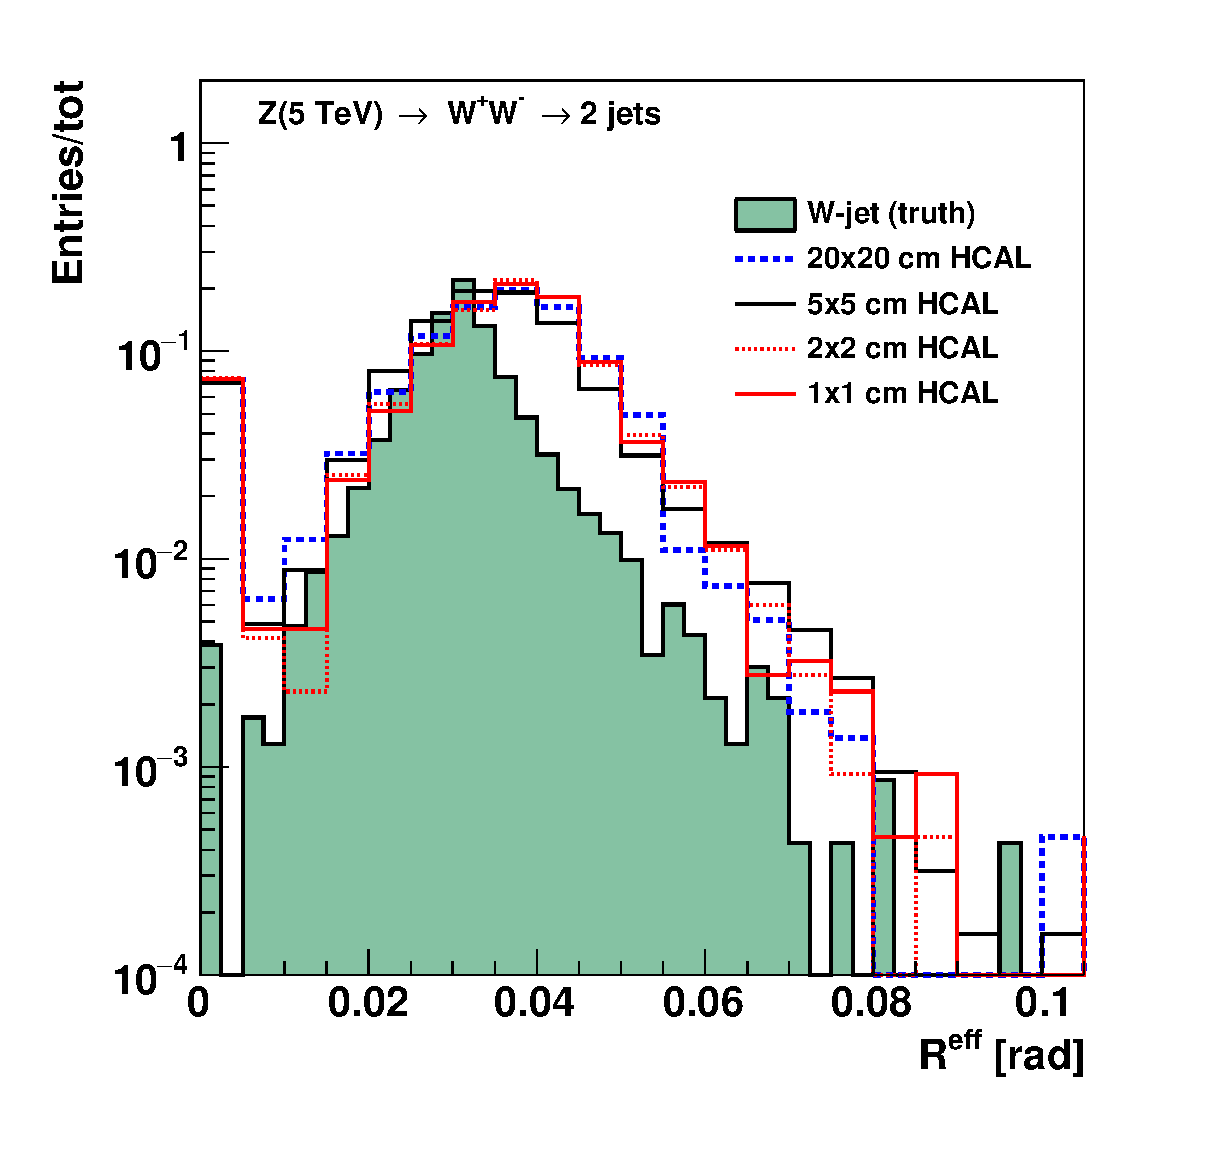
\includegraphics[width=0.43\textwidth]{figs/h5tev_clus_effR_ww1}\hfill
   }
   \subfigure[10 TeV] {
   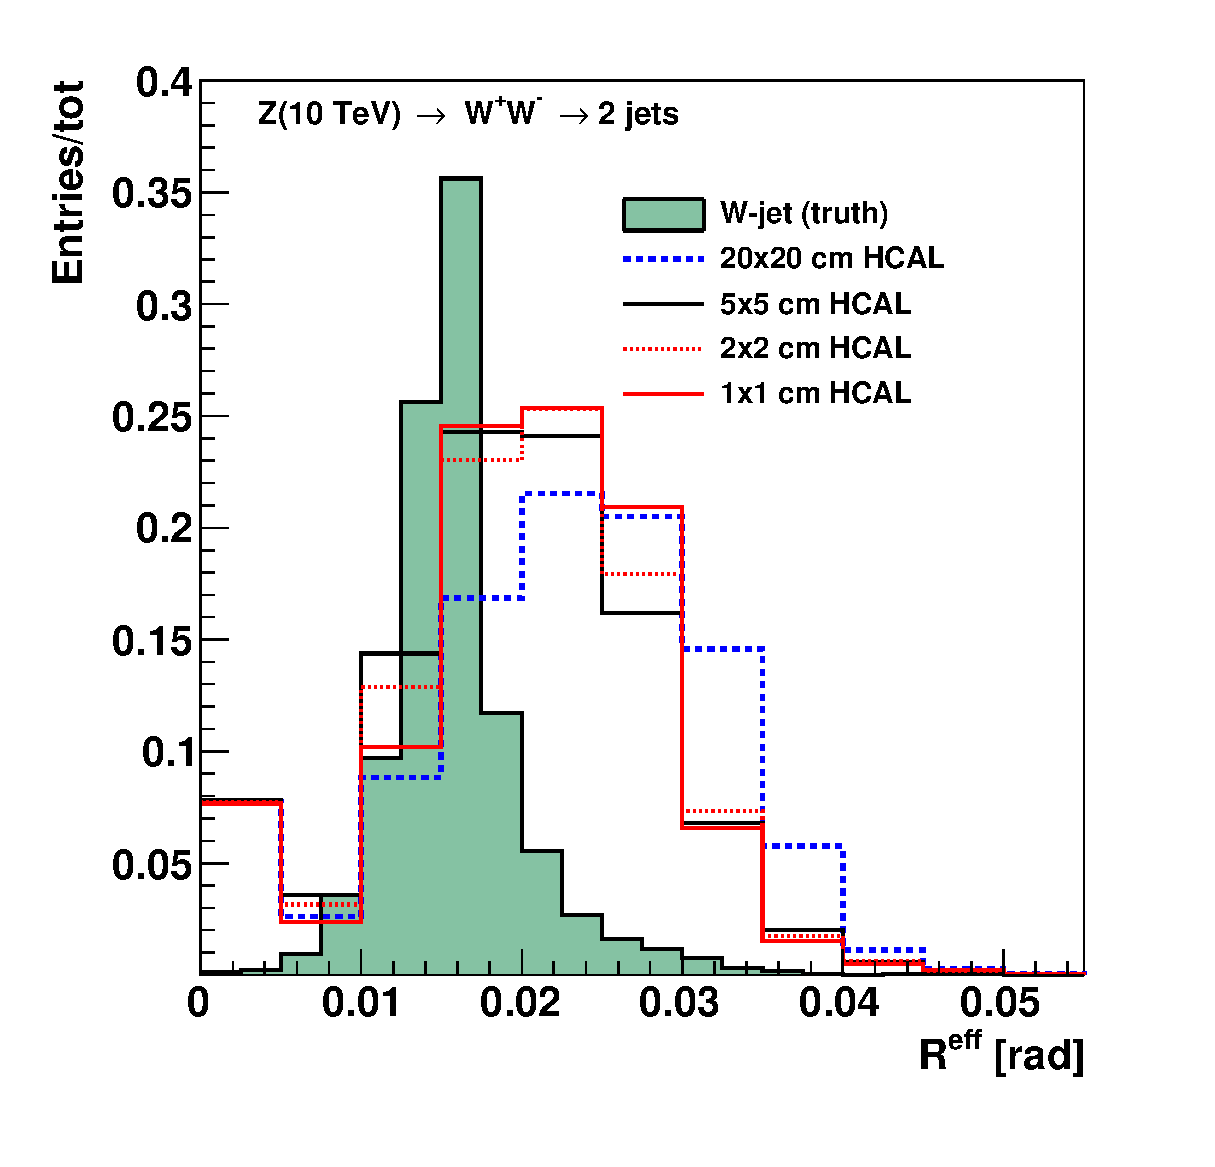
\includegraphics[width=0.43\textwidth]{figs/h10tev_clus_effR_ww1}
   }
   \subfigure[20 TeV] {
   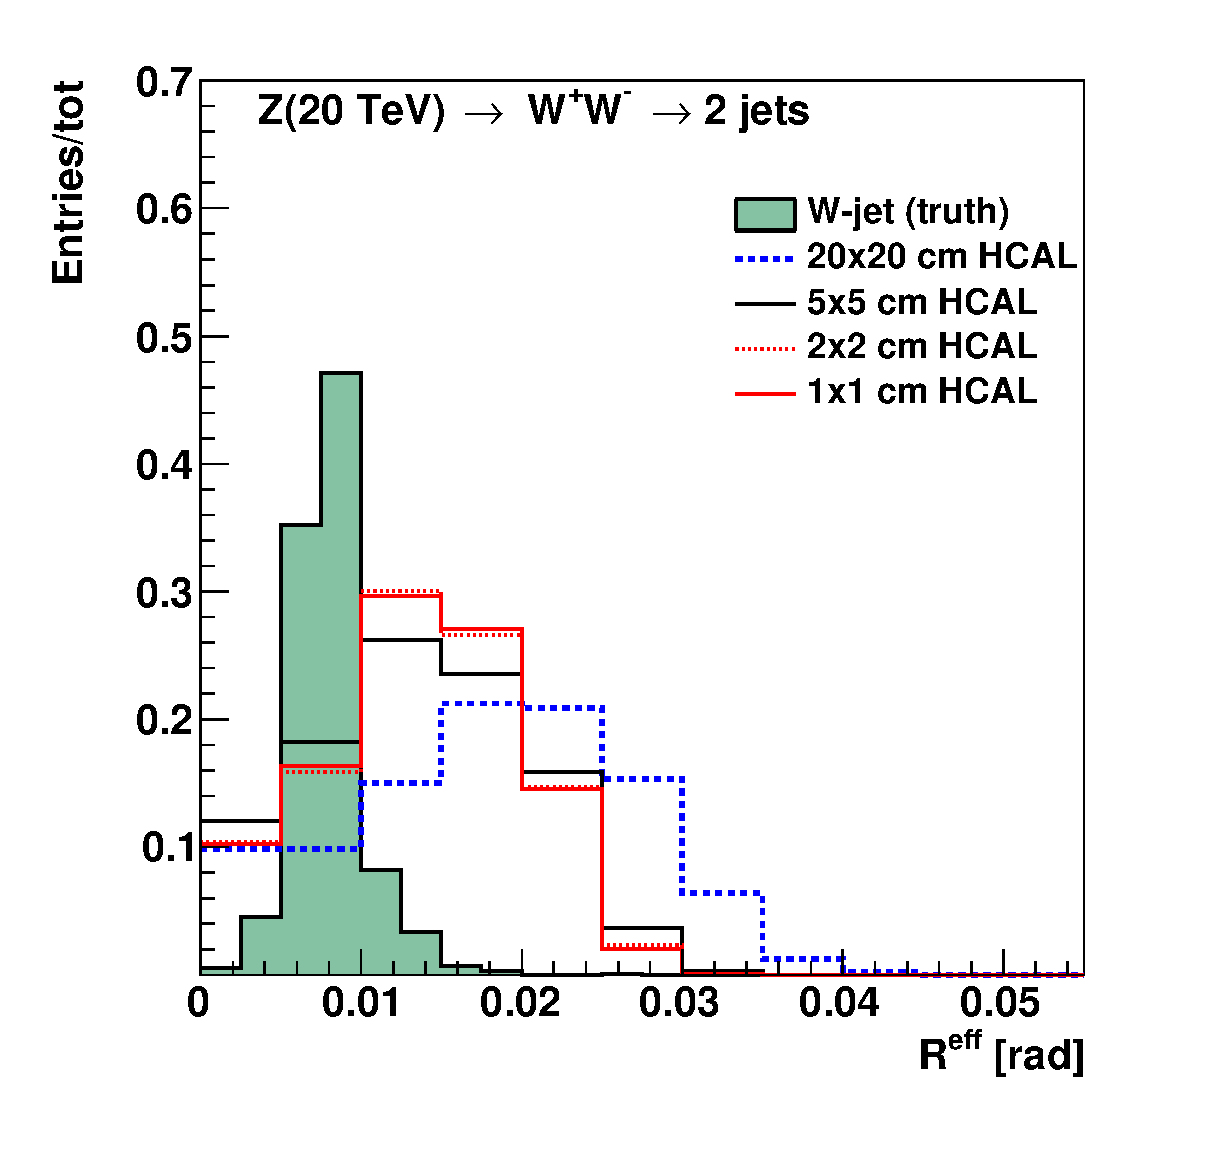
\includegraphics[width=0.43\textwidth]{figs/h20tev_clus_effR_ww1}
   }
   \subfigure[40 TeV] {
   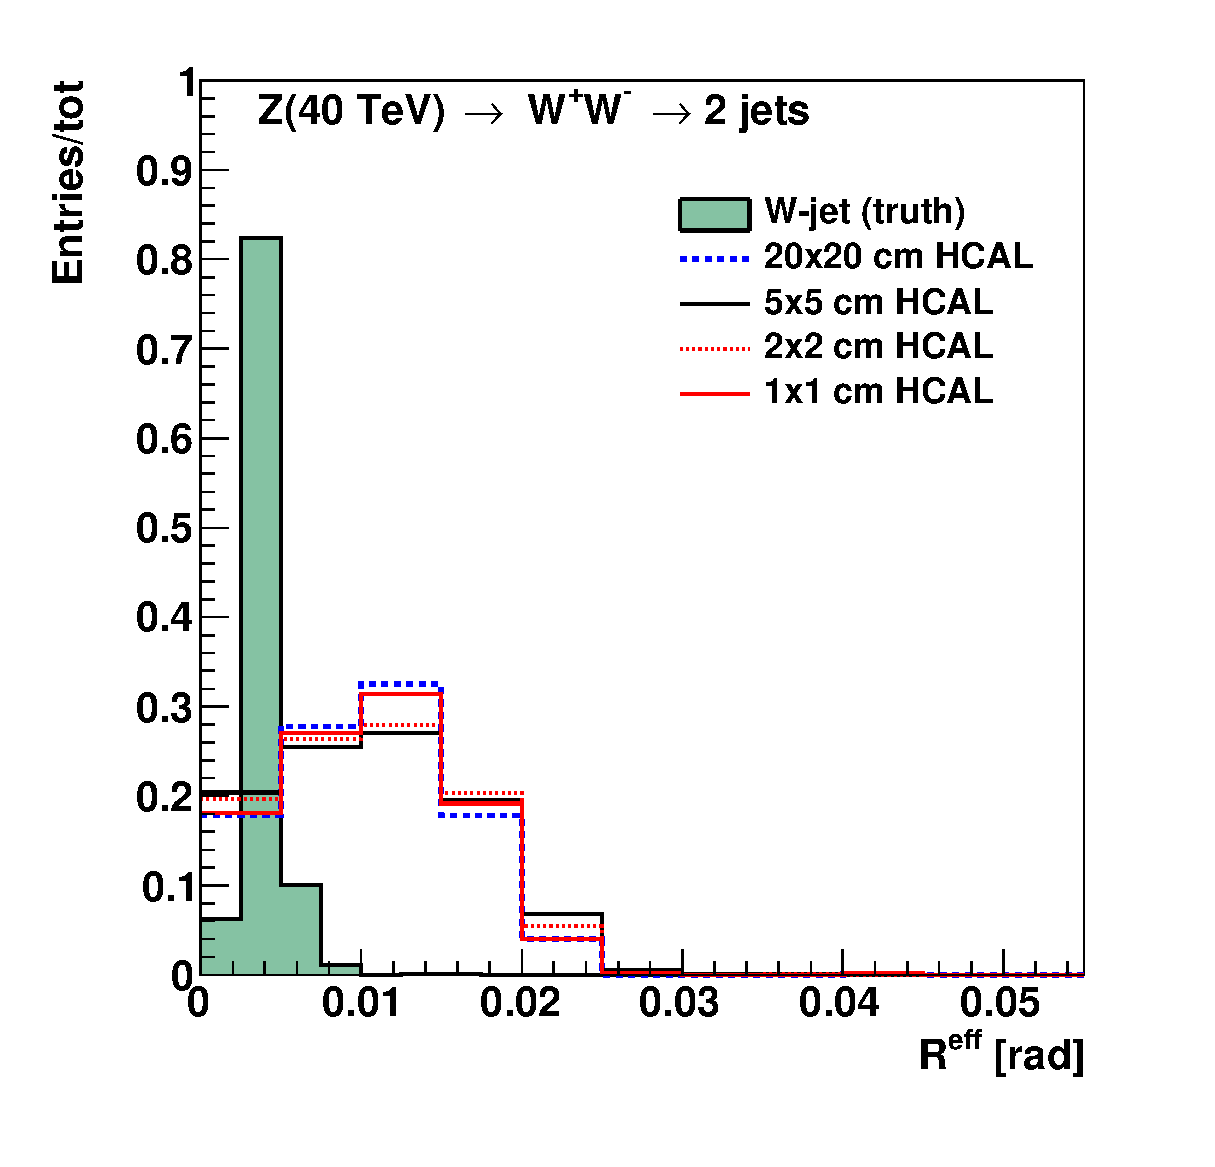
\includegraphics[width=0.43\textwidth]{figs/h40tev_clus_effR_ww1}
   }
\end{center}
\caption{Jet effective radius for different jet transverse momenta and HCAL granularities.}
\label{fig:eff_rad}
\end{figure}


Let us study the effect of granularity on jet splitting scales.
A jet $k_T$ splitting scale \cite{Butterworth:2002tt} is defined as a distance measure
used to form jets by the $k_T$ recombination
algorithm \cite{Catani1993187,Ellis:1993tq}.
This has been studied by ATLAS~\cite{ATLAS:2012am}, and more recently in the context of 100 TeV physics \cite{Auerbach:2014xua}.
The distribution of the splitting scale $\sqrt{d_{12}}=\min(p_T^1,p_T^2) \times \delta R_{12}$ \cite{ATLAS:2012am} at the final stage of the $k_T$ clustering, where two subjets are merged into the final one,
is shown in Fig.~\ref{fig:d12}.

\begin{figure}
\begin{center}
   \subfigure[5 TeV] {
   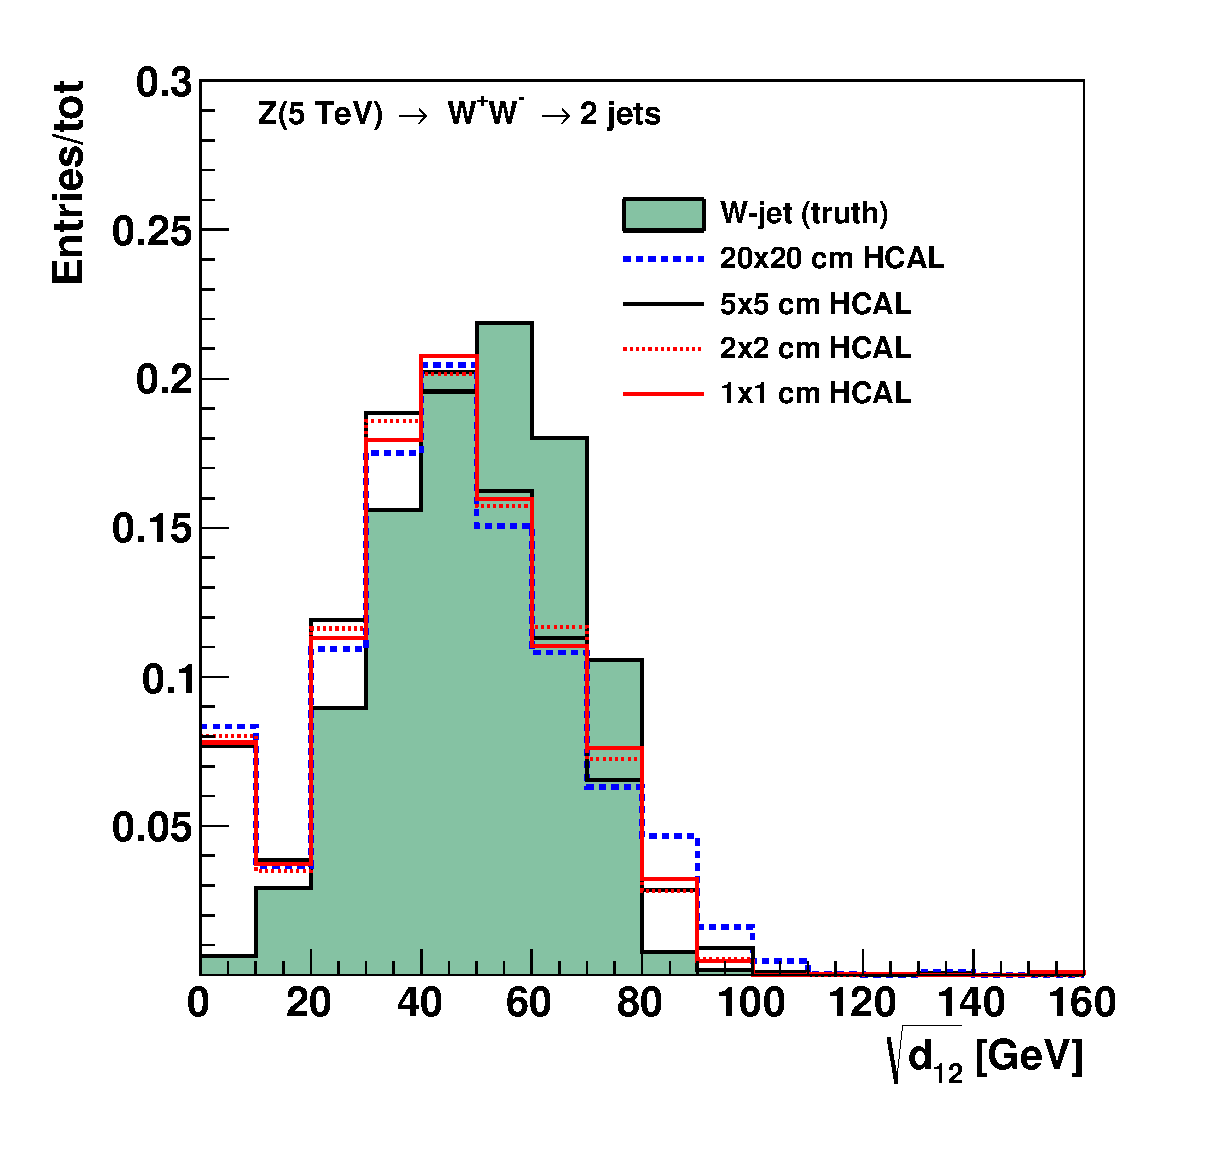
\includegraphics[width=0.43\textwidth]{figs/h5tev_clus_d12_ww1}\hfill
   }
   \subfigure[10 TeV] {
   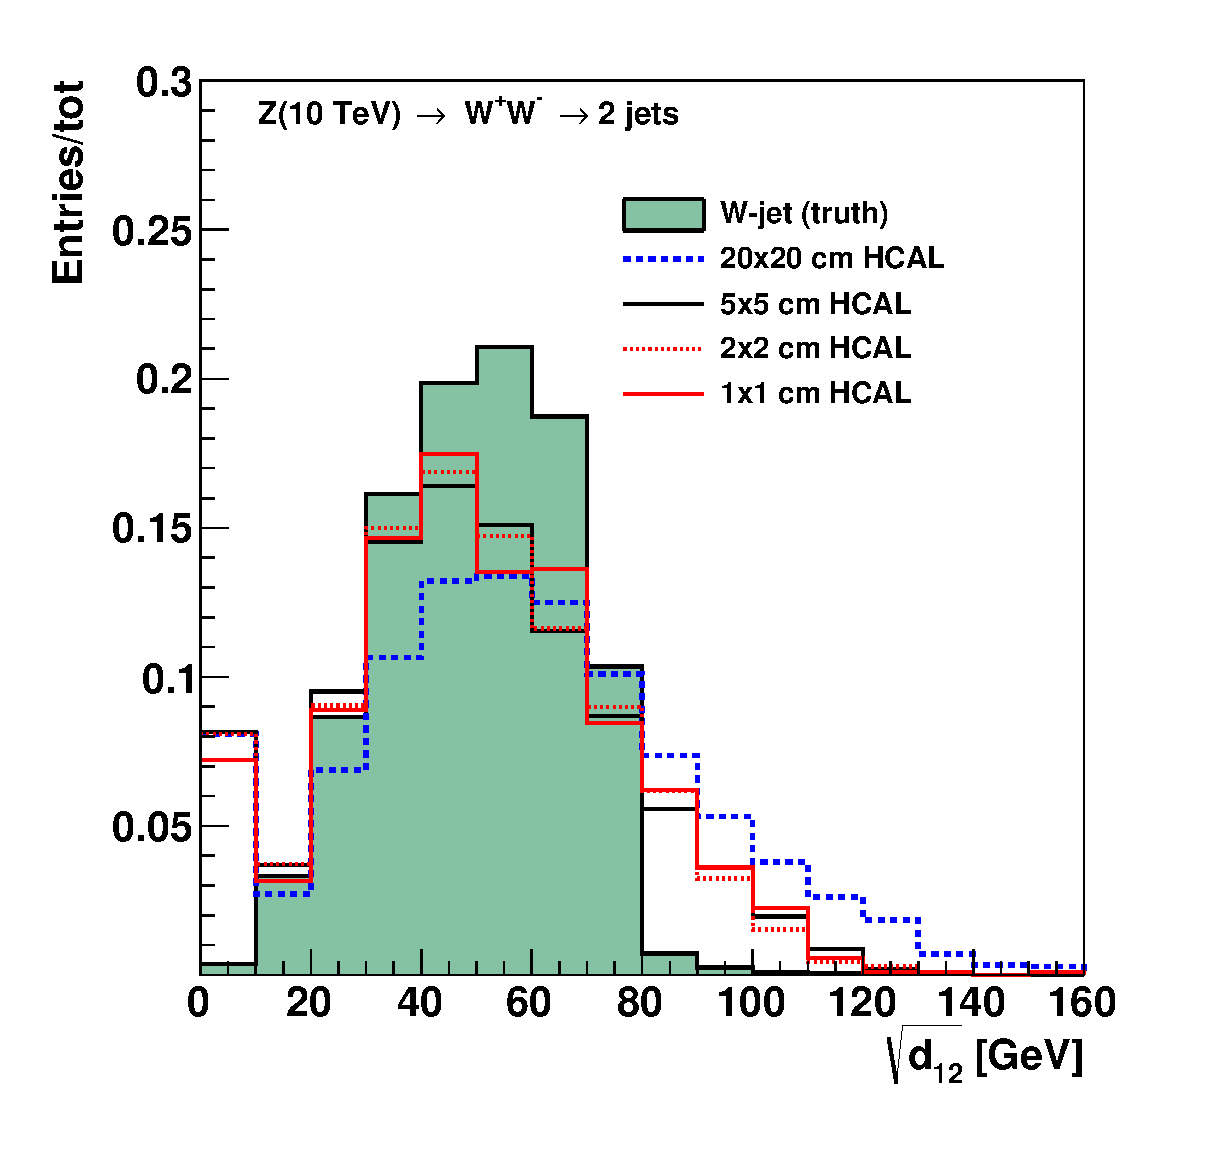
\includegraphics[width=0.43\textwidth]{figs/h10tev_clus_d12_ww1}
   }
   \subfigure[20 TeV] {
   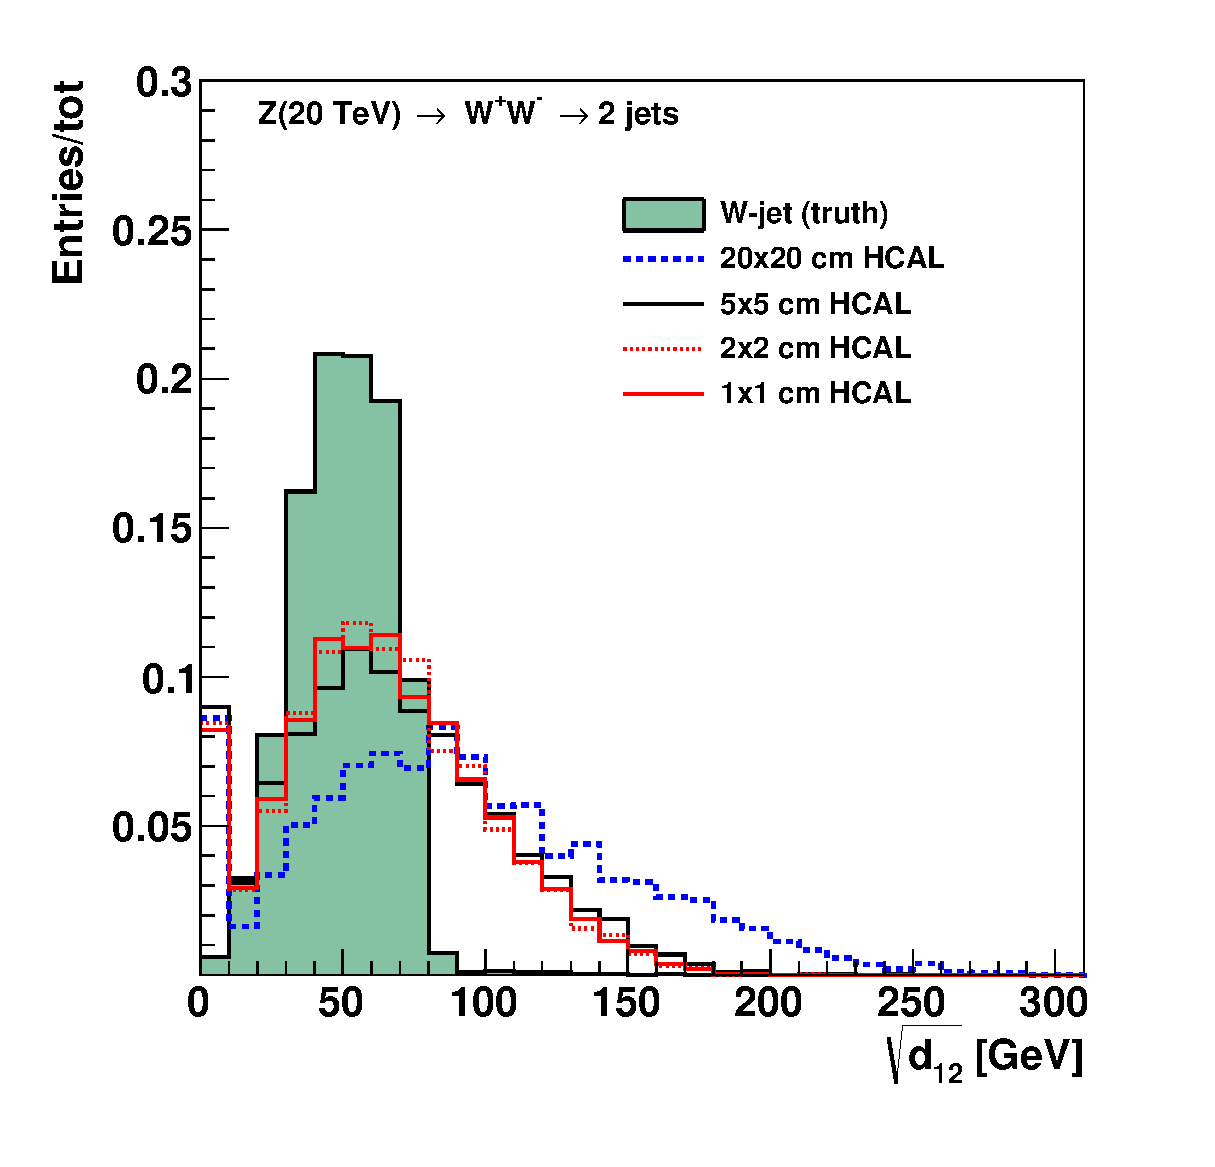
\includegraphics[width=0.43\textwidth]{figs/h20tev_clus_d12_ww1}
   }
   \subfigure[40 TeV] {
   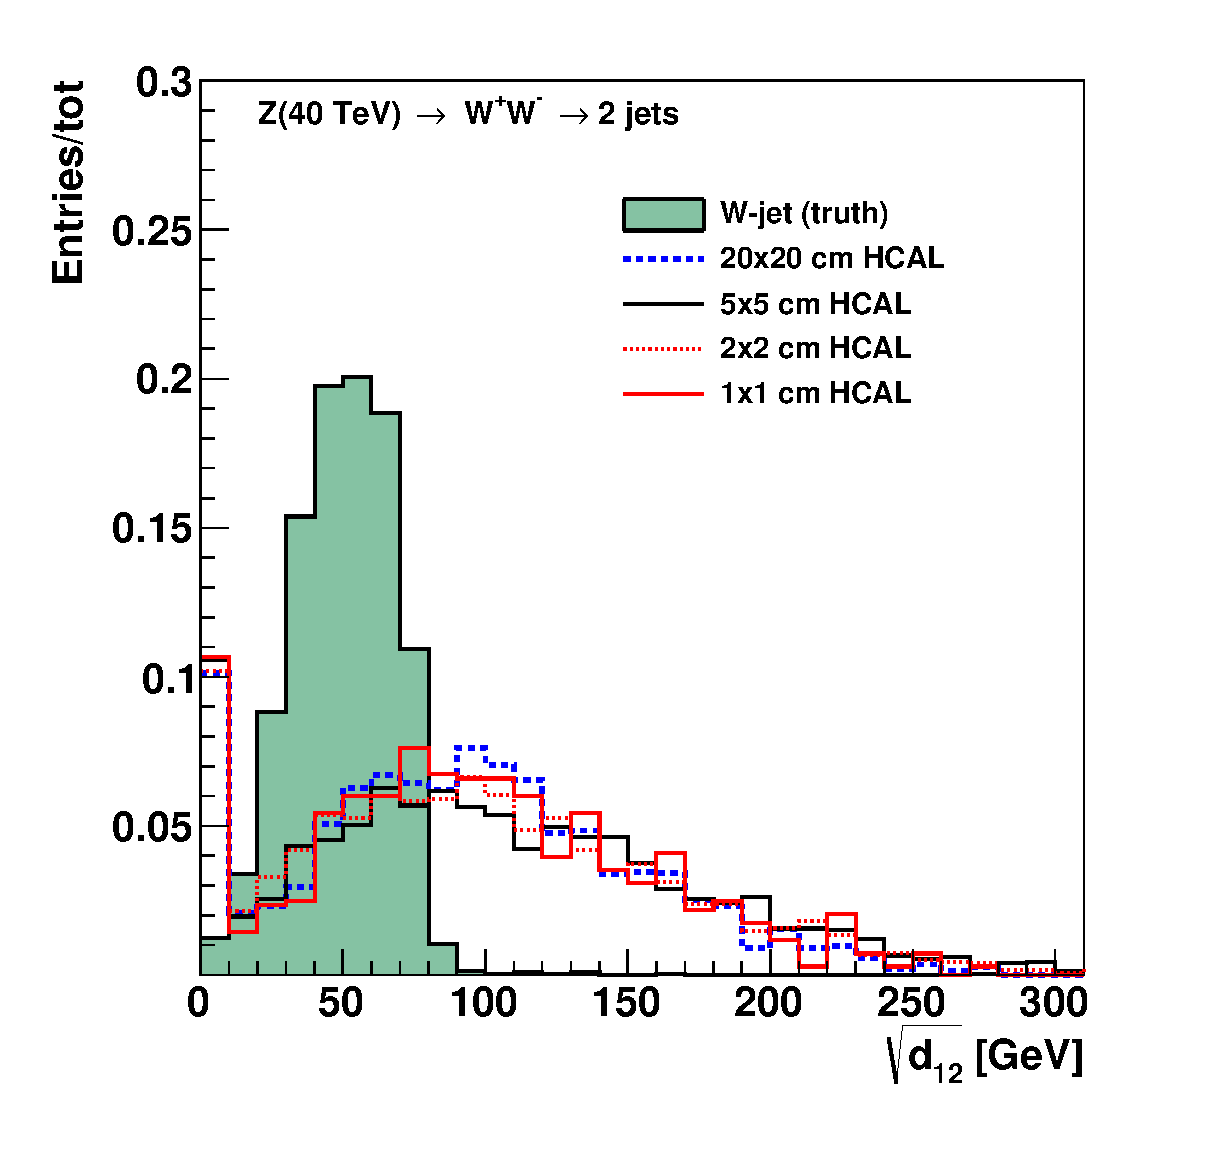
\includegraphics[width=0.43\textwidth]{figs/h40tev_clus_d12_ww1}
   }
\end{center}
\caption{Jet splitting scale for different jet transverse momenta and HCAL granularity.}
\label{fig:d12}
\end{figure}


\subsection{Jet subjettiness}

We recall that $N$-subjettiness~\cite{Thaler:2010tr}, $\tau_{N}$, of jets has been proposed
as a class of variables with which to study the decay products of a heavy particle inside jets.  $\tau_{N}$ is a measure of the degree to which a jet can be considered as being composed of
 $N$  $k_{T}$-subjets \cite{Thaler:2010tr}. 
The variable $\tau_{32}$, defined as the ratio of the $N$-subjettiness variables $\tau_3/\tau_2$, is particularly sensitive to hadronically-decaying
 top-quark initiated jets.
The variable, $\tau_{21} \equiv \tau_2/\tau_1$ can be used to reject background from $W/Z$ decays.
These variables do not strongly correlate with jet mass and can provide an independent check for the
presence of top quarks.
The jet substructure variables were obtained by re-running the $k_T$ algorithm over the jet constituents of anti-$k_T$ jets.

%%%%%%%%%%%%%%% commented out 
\begin{comment}


As an example of the effect of the calorimeter granularity, 
\begin{figure}
\begin{center}
   \subfigure[5 TeV] {
   \includegraphics[width=0.43\textwidth]{figs/r09_tau21b1_20tev_04_U.pdf}\hfill
   }
   \subfigure[10 TeV] {
   \includegraphics[width=0.43\textwidth]{figs/r010_tau21b1_20tev_04_U.pdf}
   }
   \subfigure[20 TeV] {
   \includegraphics[width=0.43\textwidth]{figs/r012_tau21b1_20tev_04_U.pdf}
   }
\end{center}
\caption{Jet subjetinness $\tau_{21}$ for jets originating from splitting scale for different jet transverse moment and HCAL granularity.}
\label{fig:tau21}
\end{figure}


\begin{figure}
\begin{center}
   \subfigure[5 TeV] {
   \includegraphics[width=0.43\textwidth]{figs/r09_tau32b1_20tev_04_U.pdf}\hfill
   }
   \subfigure[10 TeV] {
   \includegraphics[width=0.43\textwidth]{figs/r010_tau32b1_20tev_04_U.pdf}
   }
   \subfigure[20 TeV] {
   \includegraphics[width=0.43\textwidth]{figs/r012_tau32b1_20tev_04_U.pdf}
   }
\end{center}
\caption{Jet subjetinness $\tau_{32}$ for jets originating from splitting scale for different jet transverse moment and HCAL granularity.}
\label{fig:tau21}
\end{figure}

%%%%%%%%%%%%%%% commented out 
\end{comment}



\section{Study of detector performance with soft drop mass}
In this section, we use the jet mass computed with a specific algorithm, soft 
drop declustering, to study the performance of detector with various detector 
cell sizes and center-of-mass (c.m.) energies. 
\subsection{The technique of soft drop declustering}
The soft drop declustering~\cite{Larkoski:2014wba} is a grooming method 
that removes soft wide-angle radiation from a jet. The constituents of a jet 
$j_0$ are first reclustered using the Cambridge-Aachen
 (C/A) algorithm~\cite{Dokshitzer:1997in,Wobisch:1998wt}. Then, the jet $j_0$ 
is broken into two subjets $j_1$ and $j_2$ by undoing the last stage of C/A 
clustering.
If the subjets pass the following soft drop condition, jet $j_0$ is the final 
soft-drop jet. Otherwise, the algorithm redefines $j_0$ to be the subjet with 
larger $p_T$ (among $j_1$ and $j_2$) and iterates the procedure.
\begin{equation} \label{eq:soft-drop}
\frac{\mathrm{min}(p_{T1},p_{T2})}{p_{T1}+p_{T2}}>z_\mathrm{cut}(\frac{\Delta R_{12}}{R_{0}})^{\beta},
\end{equation}
where $p_{T1}$ and $p_{T2}$ are the transverse momenta of the two subjets, 
$z_\mathrm{cut}$ is soft drop threshold, 
$\Delta R_{12}$ is the distance between the two subjets in the 
rapidity-azimuth angle plane ($y$-$\phi$), $R_0$ is the characteristic radius 
of the original jet, and $\beta$ is the angular exponent.

In our study, we compare the performance of future detector when setting 
$\beta=0$ versus when setting $\beta=2$. For $\beta=0$, the soft drop condition 
depends only on the $z_\mathrm{cut}$. For $\beta=2$, the condition depends on 
the angular distance between the two subjets and $z_\mathrm{cut}$ and the 
algorithm becomes infrared and collinear safe. 

\subsection{Analysis method \label{sec:massana}}
We employ the following method to quantify the detector performance and 
find out the cell size that gives the best separation power to distinguish 
signal from background. For each configuration of detector and c.m. energy, 
we draw the receiver operating characteristic (ROC) curves in which the x-axis
 is the signal efficiency ($\epsilon_\mathrm{sig}$) and y-axis is the inverse 
of background efficiency ($1/\epsilon_\mathrm{bkg}$). 
In order to scan the efficiencies of soft drop mass cuts, we vary the mass 
window as follows. We first look for the median bin 
$i_\mathrm{med}$\footnote{The integral from bin 0 to bin $i_\mathrm{med}$ 
($i_\mathrm{med}-1$) should be greater (less) than half 
of the total number of events. Note, the bin width is 5~GeV.} of the soft 
drop mass histogram from simulated signal events. Taking the right boundary
 of bin $i_\mathrm{med}$ as the center of mass window 
$x_\mathrm{center}$, we start increasing the width of mass window symmetrically
 on the left and on the right of $x_\mathrm{center}$, in steps of 5~GeV, 
i.e. the narrowest mass window is 
[$x_\mathrm{center}-5,x_\mathrm{center}+5$]. If one side reaches the boundary 
of the mass histogram, we only increase the width on the other side, also in 
steps of 5~GeV. For each mass window, there will be corresponding 
$\epsilon_\mathrm{sig}$ and $\epsilon_\mathrm{bkg}$, which gives a point in 
the ROC curves.

\subsection{Results and conclusion}
Figures~\ref{fig:cluster_mass_mmdt_ww}, \ref{fig:cluster_mass_mmdt_tt},
 \ref{fig:cluster_mass_sdb2_ww}, and \ref{fig:cluster_mass_sdb2_tt} 
present the distributions of soft drop mass for $\beta=0$ and $\beta=2$ with 
different c.m. energies and detector cell sizes; the signals considered are 
Z'$\rightarrow$WW and Z'$\rightarrow$t$\bar{\mathrm{t}}$. 
In Figs.~\ref{fig:cluster_mass_mmdt_ww_ROC}, \ref{fig:cluster_mass_mmdt_tt_ROC}, \ref{fig:cluster_mass_sdb2_ww_ROC}, and \ref{fig:cluster_mass_sdb2_tt_ROC}, 
ROC curves from different detector cell sizes are compared for each 
c.m. energy, respectively. 

Figures~\ref{fig:cluster_mass_mmdt_ww_ROC} and 
\ref{fig:cluster_mass_mmdt_tt_ROC} show that for $\beta=0$ the 
smallest detector cell size, 
 $1~\mathrm{cm}\times1~\mathrm{cm}$, has the best separation power at 
$\sqrt{s}=$5, 10, and 20 TeV when the signal is Z'$\rightarrow$WW and 
at  $\sqrt{s}=$10 and 20 TeV when the signal is Z'$\rightarrow$t$\bar{\mathrm{t}}$.
On the contrary, Figs.~\ref{fig:cluster_mass_sdb2_ww_ROC} and \ref{fig:cluster_mass_sdb2_tt_ROC} show that for $\beta=2$ the smallest detector cell size 
does not have improvements in the separation power with respect to those with 
larger cell sizes. In fact, the performances of the three cell sizes are 
similar. In addition, sometimes bigger detector cell sizes, 
$5~\mathrm{cm}\times5~\mathrm{cm}$ or $20~\mathrm{cm}\times20~\mathrm{cm}$
 have the best separation power. 

We also find compared to $\beta=2$, soft drop mass with $\beta=0$ has better 
performance for distinguishing signal from background. Therefore, we will 
apply requirements on this variable when studying the other jet substructure 
variables. 
 
%50bins
\begin{figure}
\begin{center}
   \subfigure[20$\times$20($cm^2$)] {
   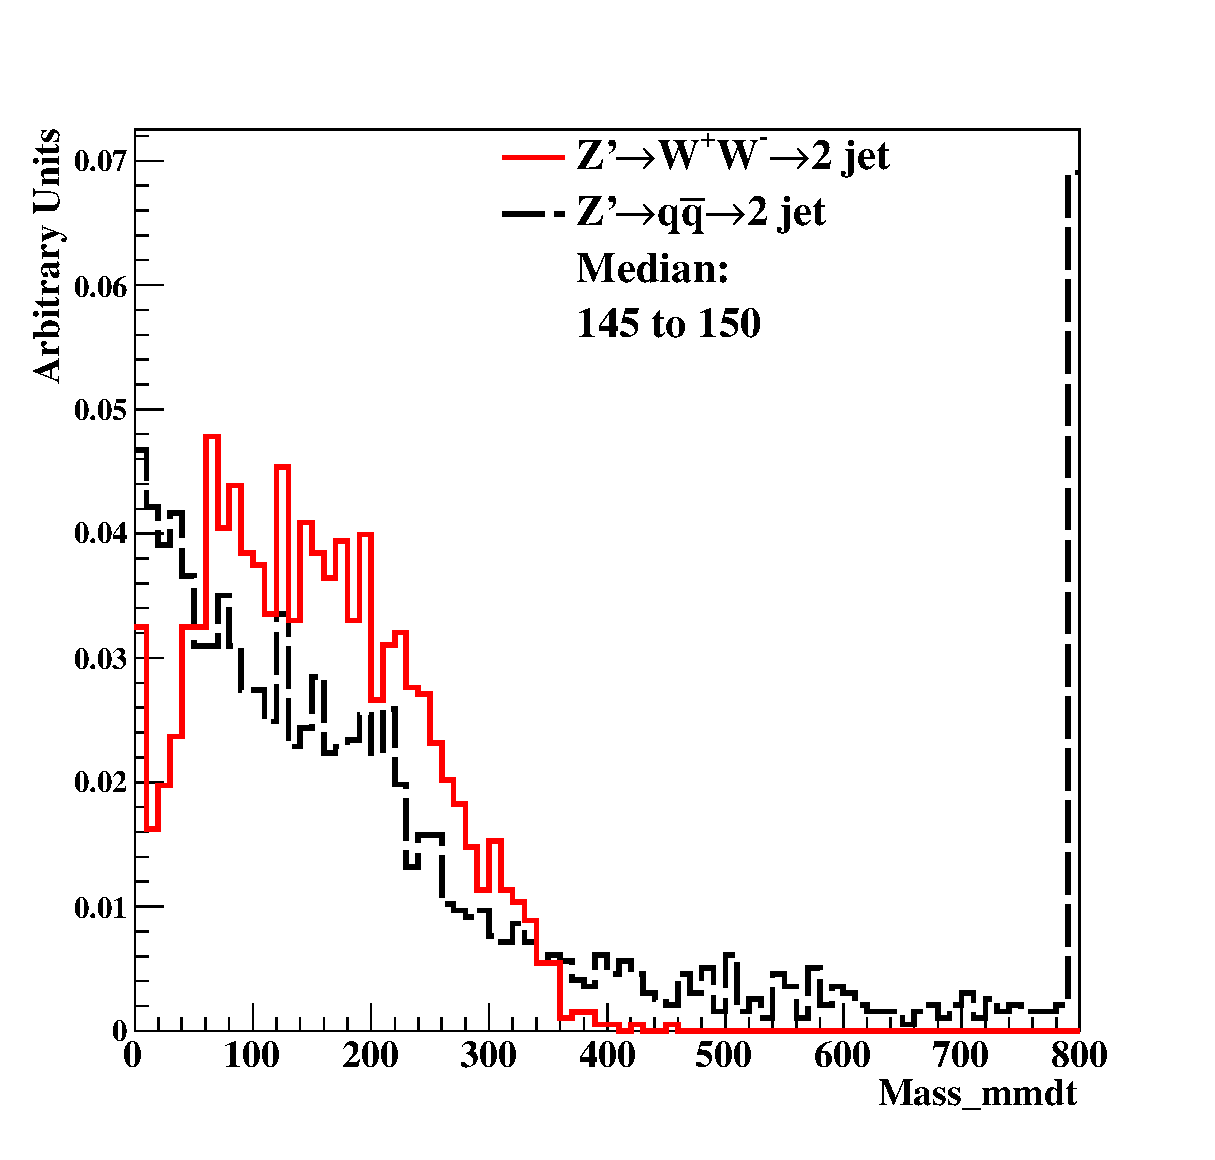
\includegraphics[ width=0.3\textwidth]{h_soft_drop/Dis_cluster_010_mass_mmdt_20tev_04_no_UOF.eps}
   }
      \subfigure[5$\times$5($cm^2$)] {
   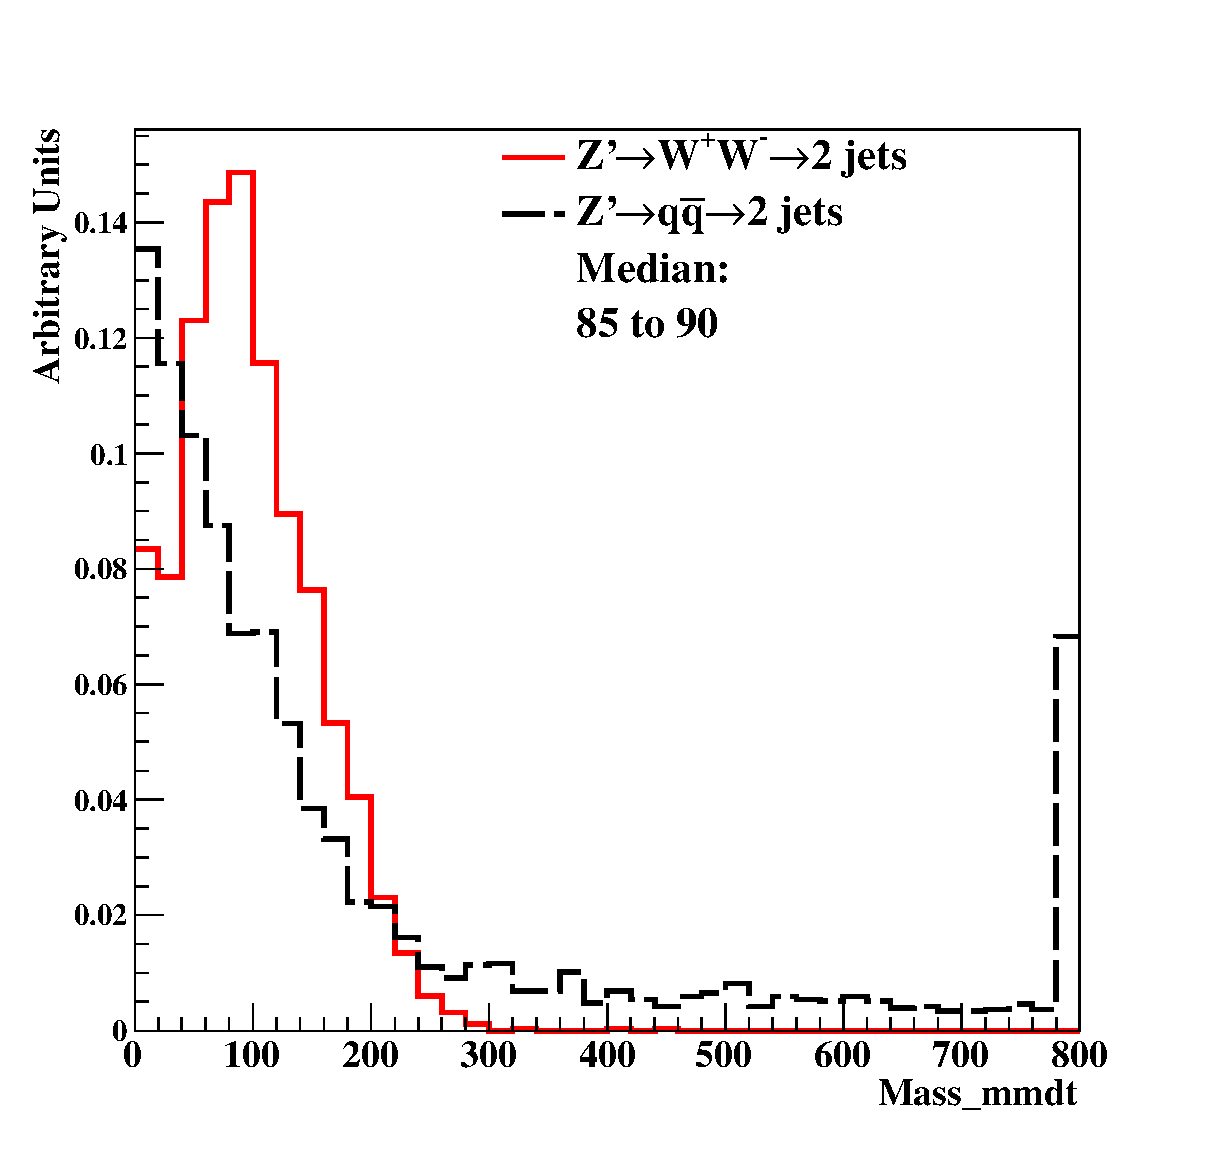
\includegraphics[ width=0.3\textwidth]{h_soft_drop/Dis_cluster_009_mass_mmdt_20tev_04_no_UOF.eps}\hfill
   }
   \subfigure[1$\times$1($cm^2$)] {
   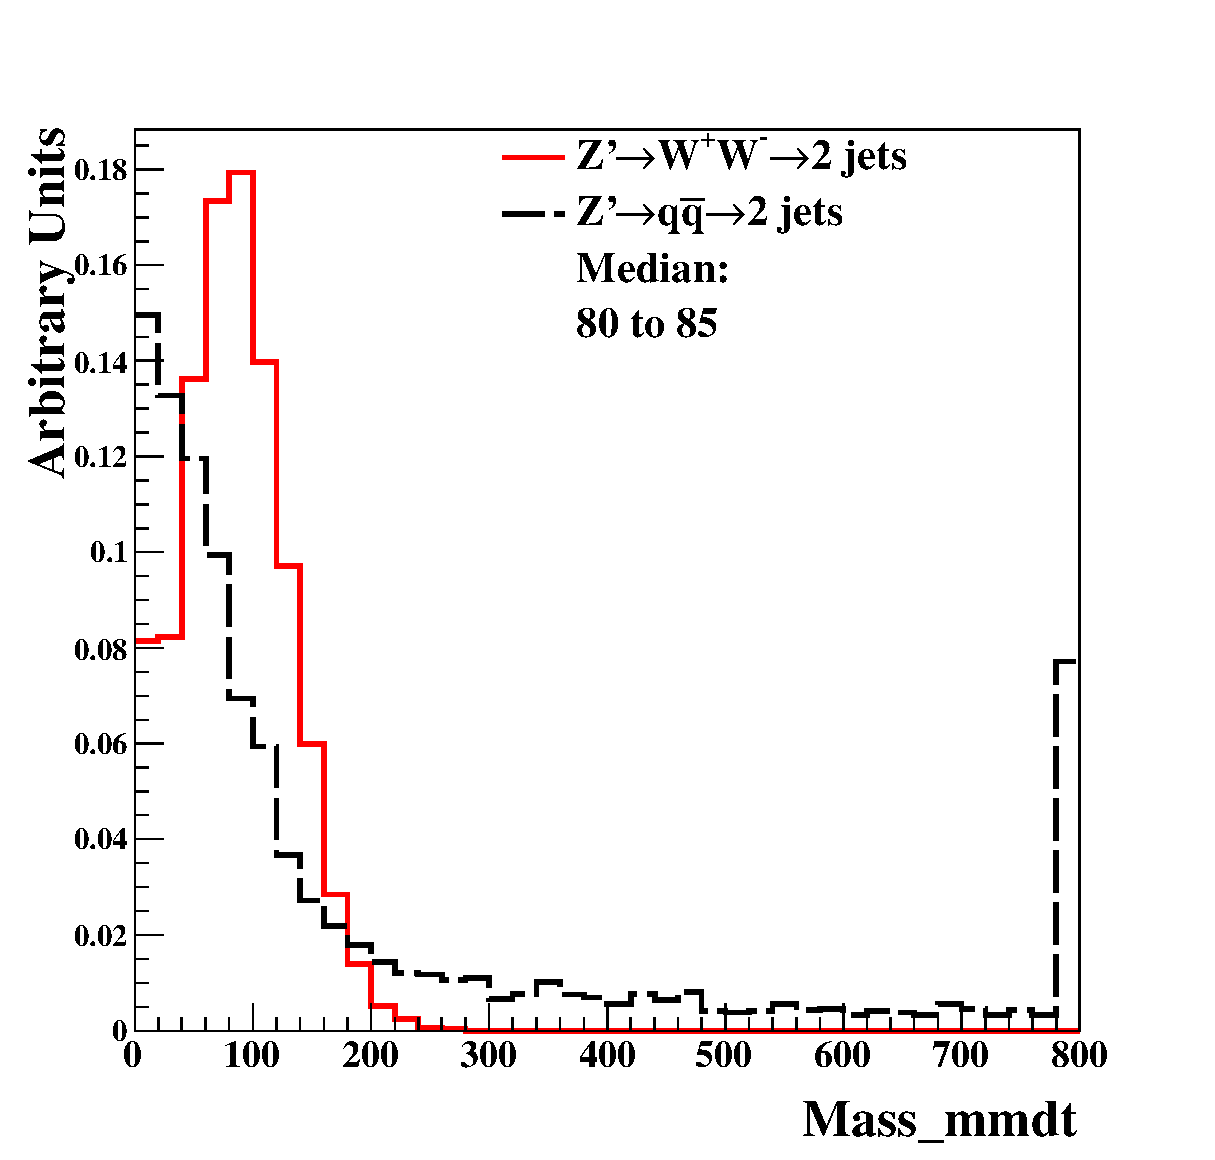
\includegraphics[ width=0.3\textwidth]{h_soft_drop/Dis_cluster_012_mass_mmdt_20tev_04_no_UOF.eps}\hfill
   }
\end{center}
\caption{Distributions of soft drop mass for $\beta$=0, with 20 TeV c.m. energies and three different detector cell sizes: 20$\times$20, 
5$\times$5, and 1$\times$1 ($cm^2$). The signal (background) process is 
Z'$\rightarrow$WW (Z'$\rightarrow$q$\bar{\mathrm{q}}$).
\label{fig:cluster_mass_mmdt_ww}}
\end{figure}


\begin{figure}
\begin{center}
  \subfigure[Z'(5 TeV)] {
  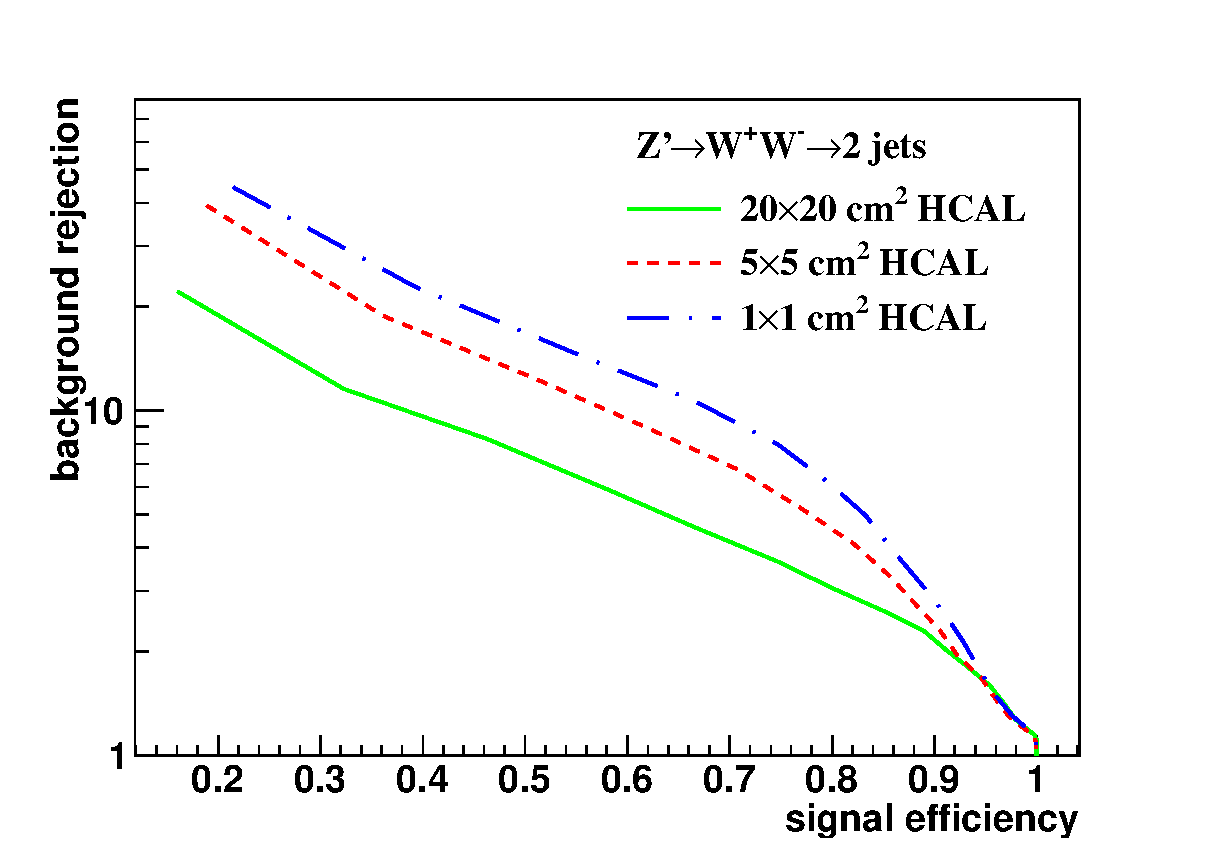
\includegraphics[  width=0.45\textwidth]{ROC_soft_drop/A_Cluster_mass_mmdt_5tev_eff_1_central_fix_at_Median_bin_ww_qq_log_no_UOF.eps}
  }
  \subfigure[Z'(10 TeV)] {
  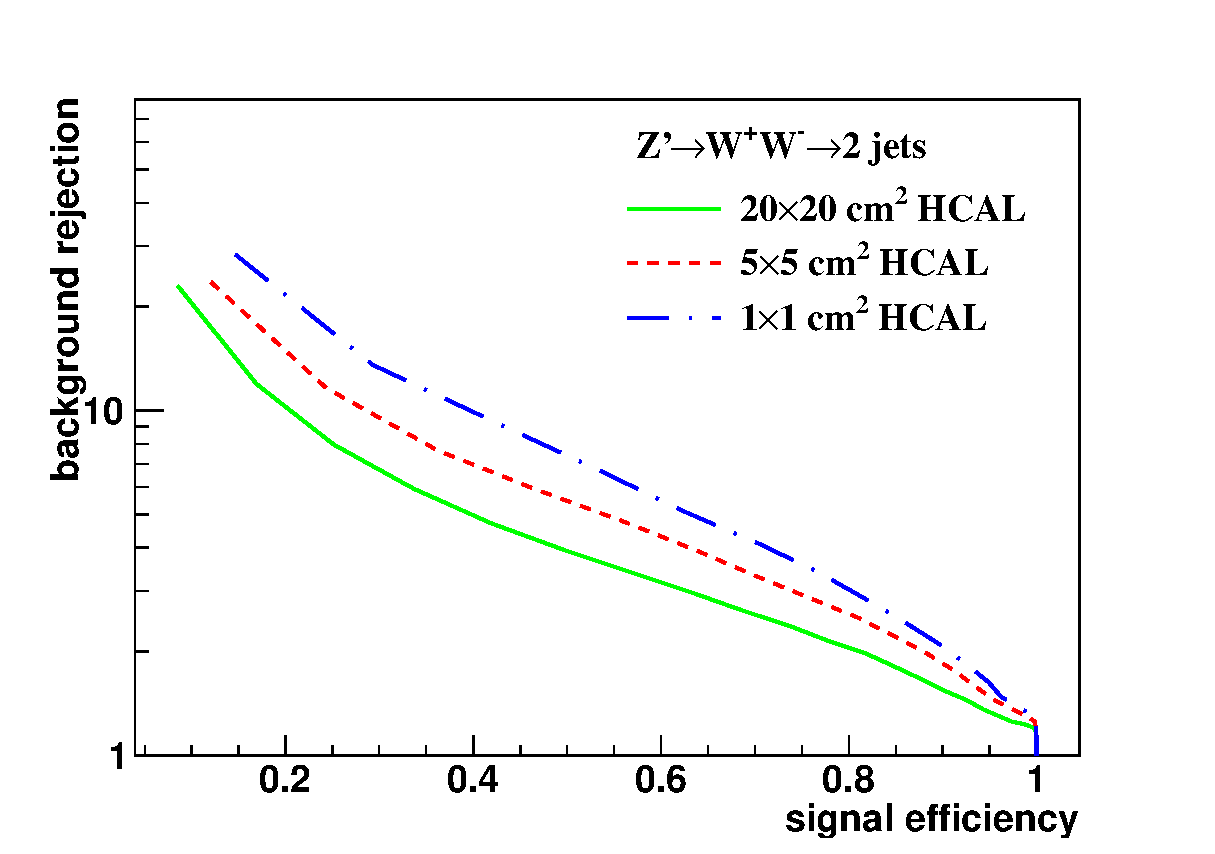
\includegraphics[  width=0.45\textwidth]{ROC_soft_drop/A_Cluster_mass_mmdt_10tev_eff_1_central_fix_at_Median_bin_ww_qq_log_no_UOF.eps}
  }
 \subfigure[Z'(20 TeV)] {
 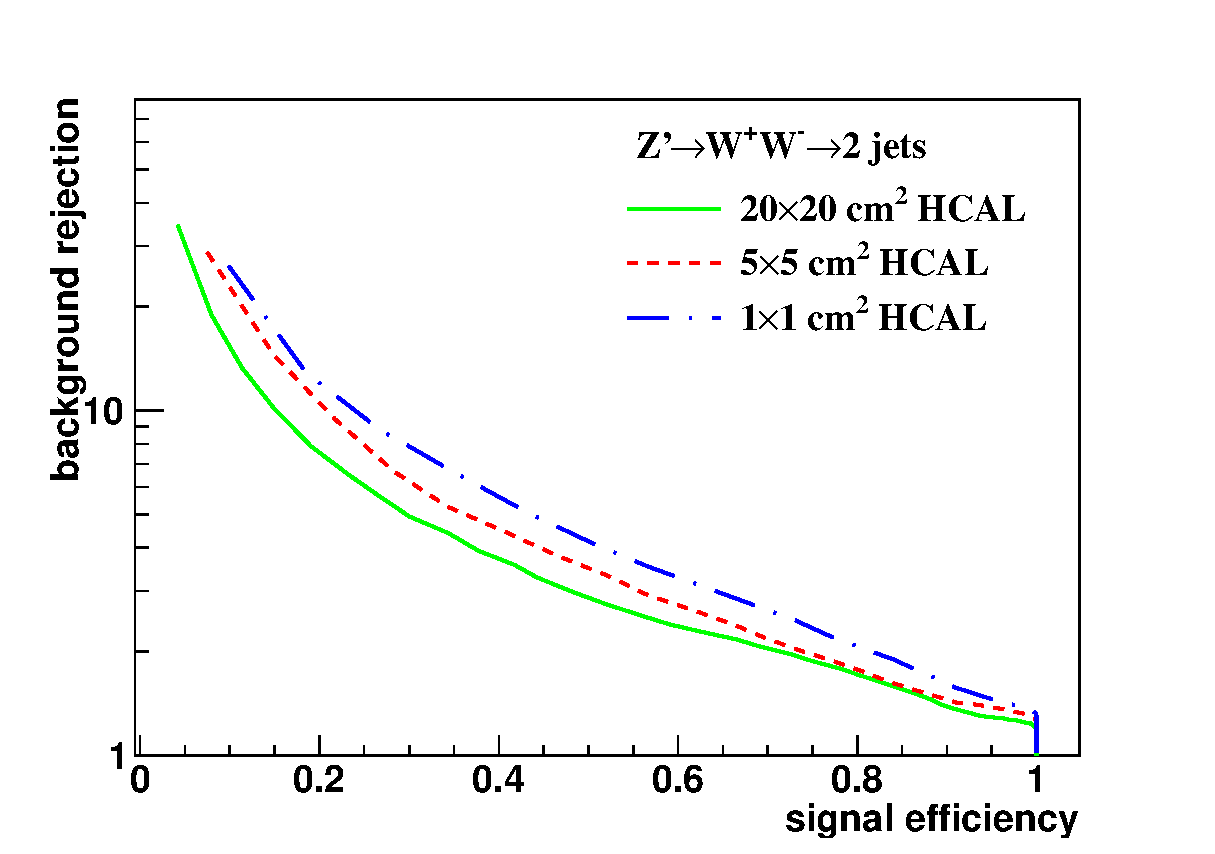
\includegraphics[  width=0.45\textwidth]{ROC_soft_drop/A_Cluster_mass_mmdt_20tev_eff_1_central_fix_at_Median_bin_ww_qq_log_no_UOF.eps}
 }
 \subfigure[Z'(40 TeV)] {
 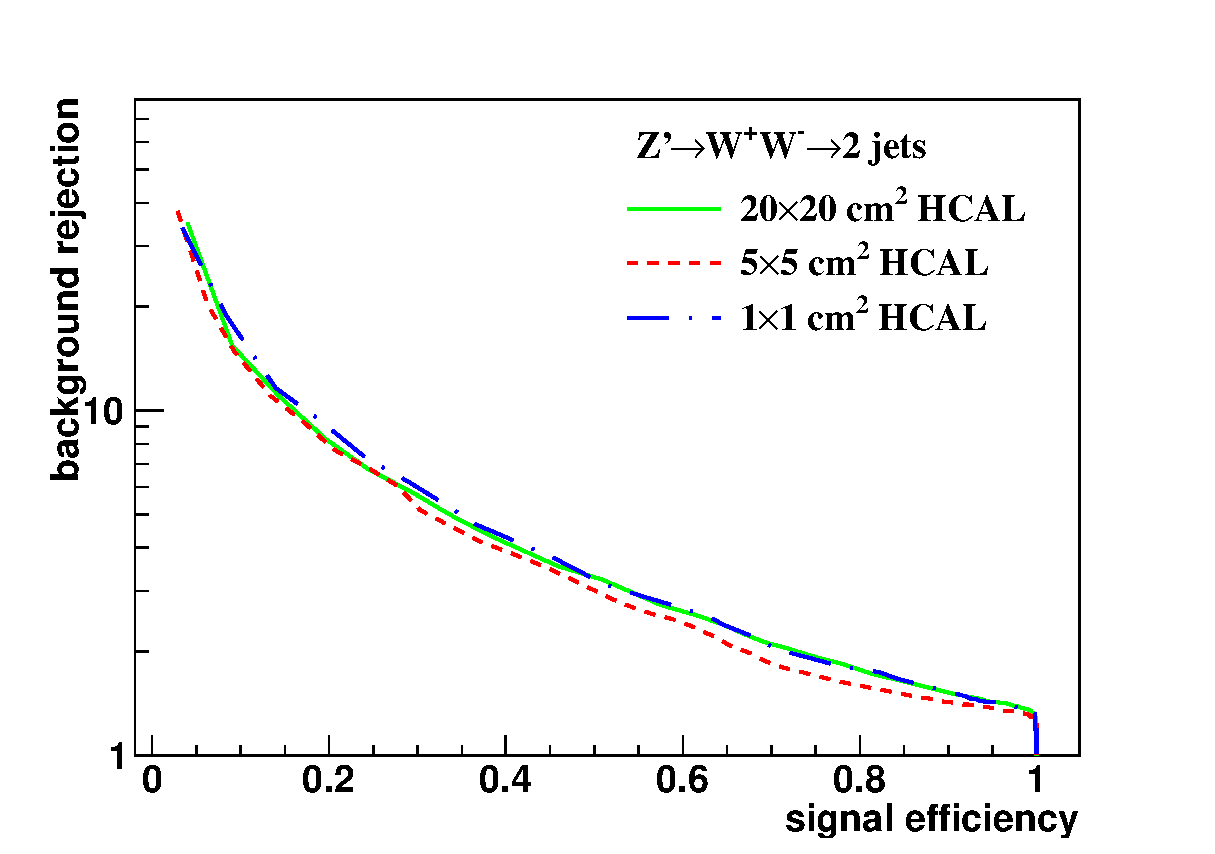
\includegraphics[  width=0.45\textwidth]{ROC_soft_drop/A_Cluster_mass_mmdt_40tev_eff_1_central_fix_at_Median_bin_ww_qq_log_no_UOF.eps}
 }
\end{center}
\caption{The ROC curves of soft drop mass selection for $\beta$=0 
with 5, 10, 20, 40 TeV c.m. energies. 
Three different detector cell sizes are compared: 20$\times$20, 
5$\times$5, and 1$\times$1 ($cm^2$). 
The signal (background) process is Z'$\rightarrow$WW 
(Z'$\rightarrow$q$\bar{\mathrm{q}}$).}
\label{fig:cluster_mass_mmdt_ww_ROC}
\end{figure}


\begin{figure}
\begin{center}
   \subfigure[5$\times$5 ($cm^2$)] {
   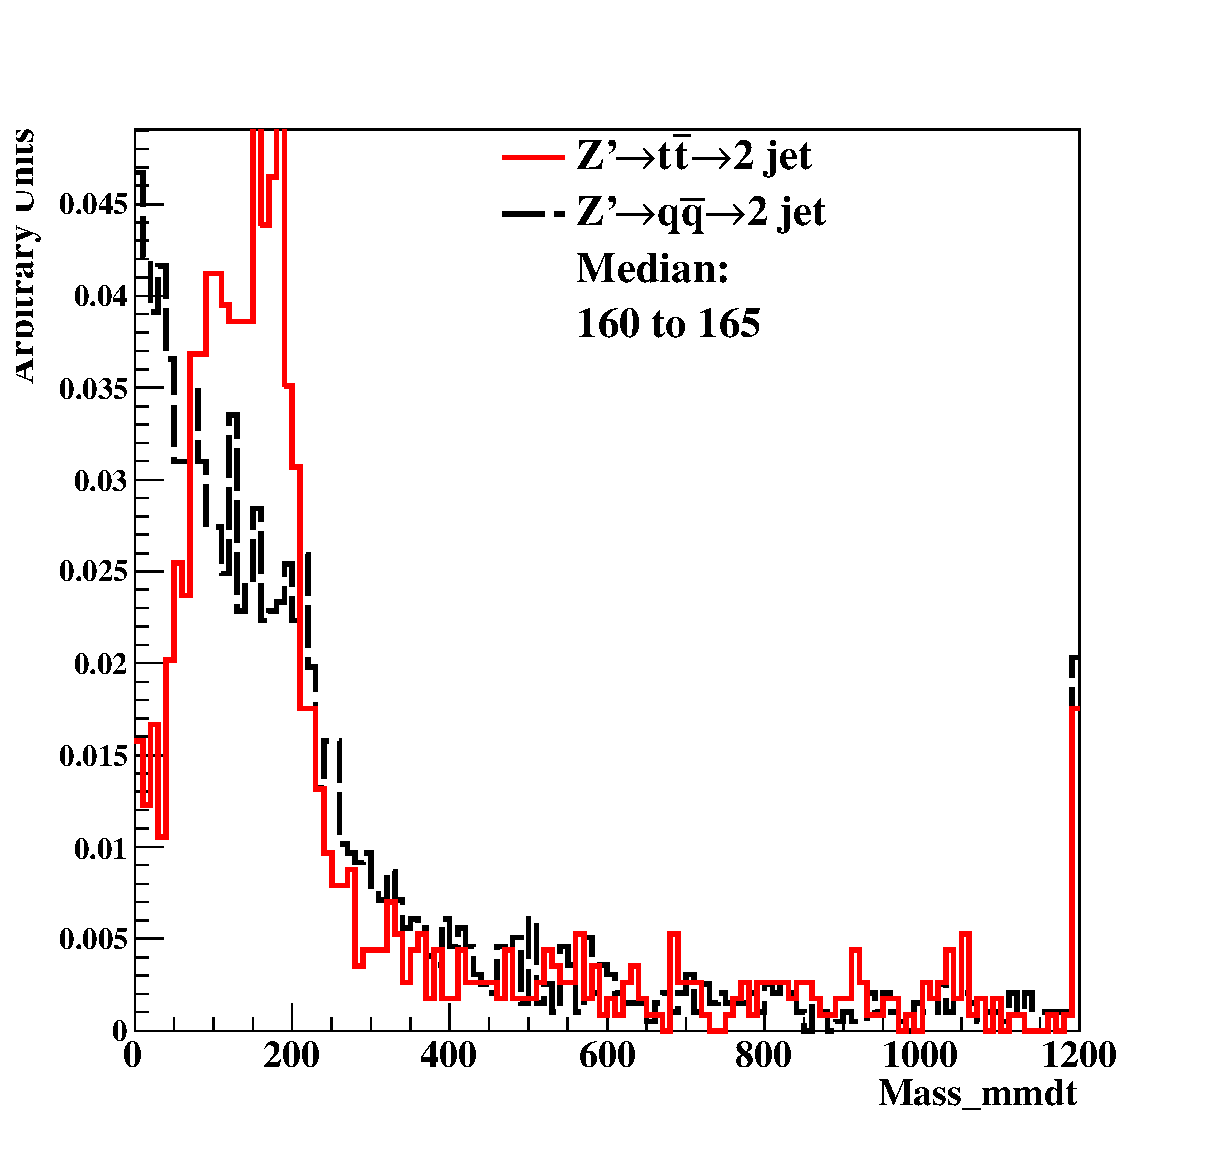
\includegraphics[   width=0.3\textwidth]{h_soft_drop/Dis_cluster_010_mass_mmdt_tt_20tev_04_tt_no_UOF.eps}
   }
   \subfigure[20$\times$20 ($cm^2$)] {
   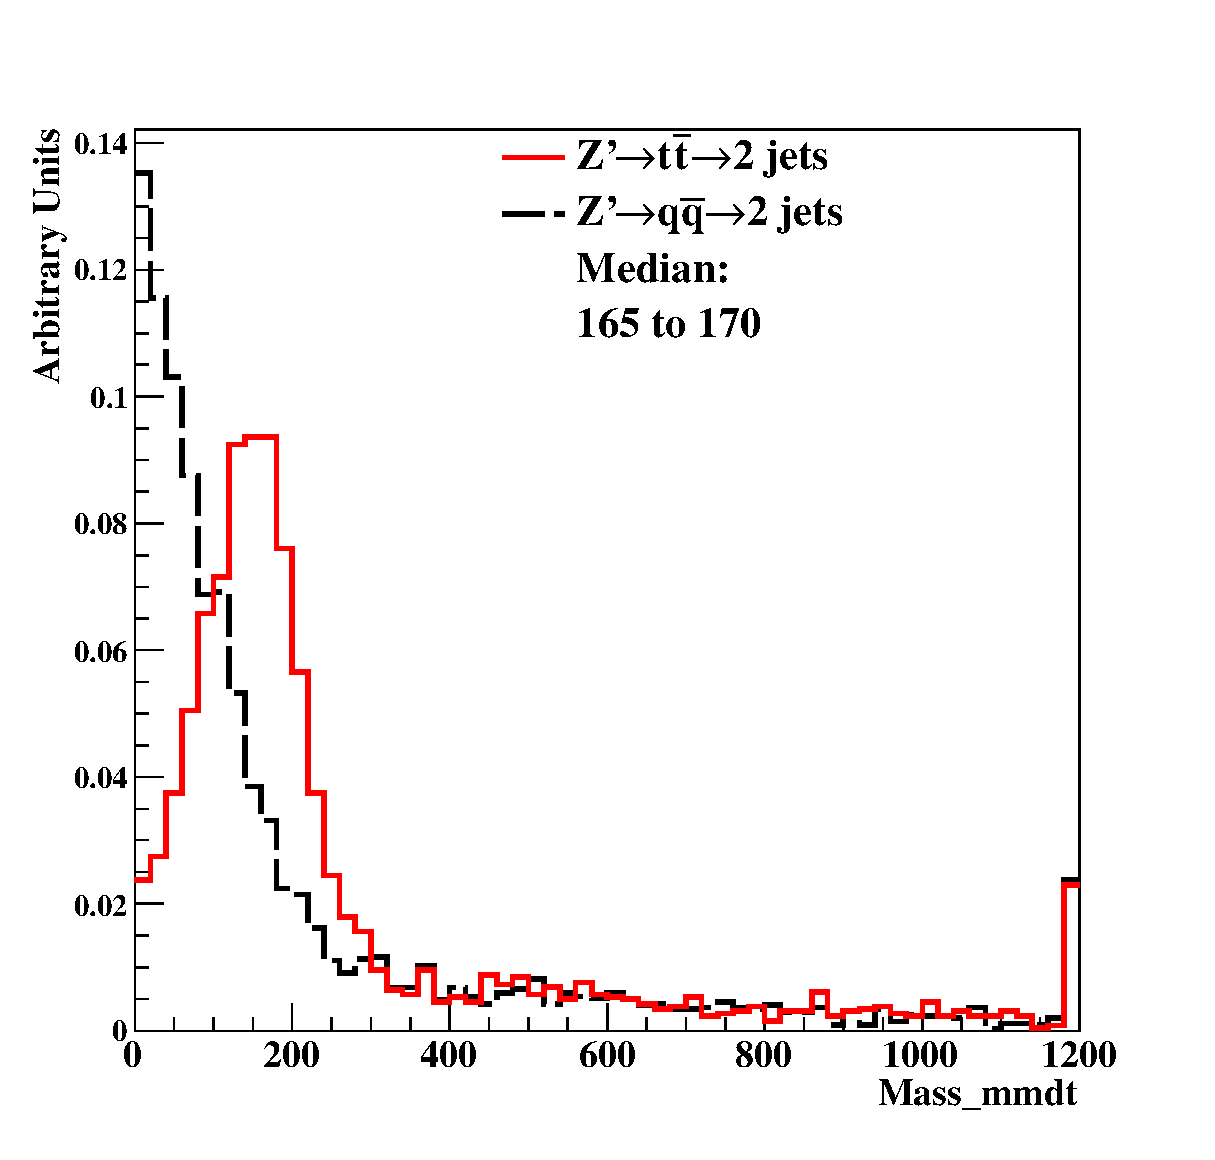
\includegraphics[   width=0.3\textwidth]{h_soft_drop/Dis_cluster_009_mass_mmdt_tt_20tev_04_tt_no_UOF.eps}\hfill
   }
   \subfigure[1$\times$1 ($cm^2$)] {
   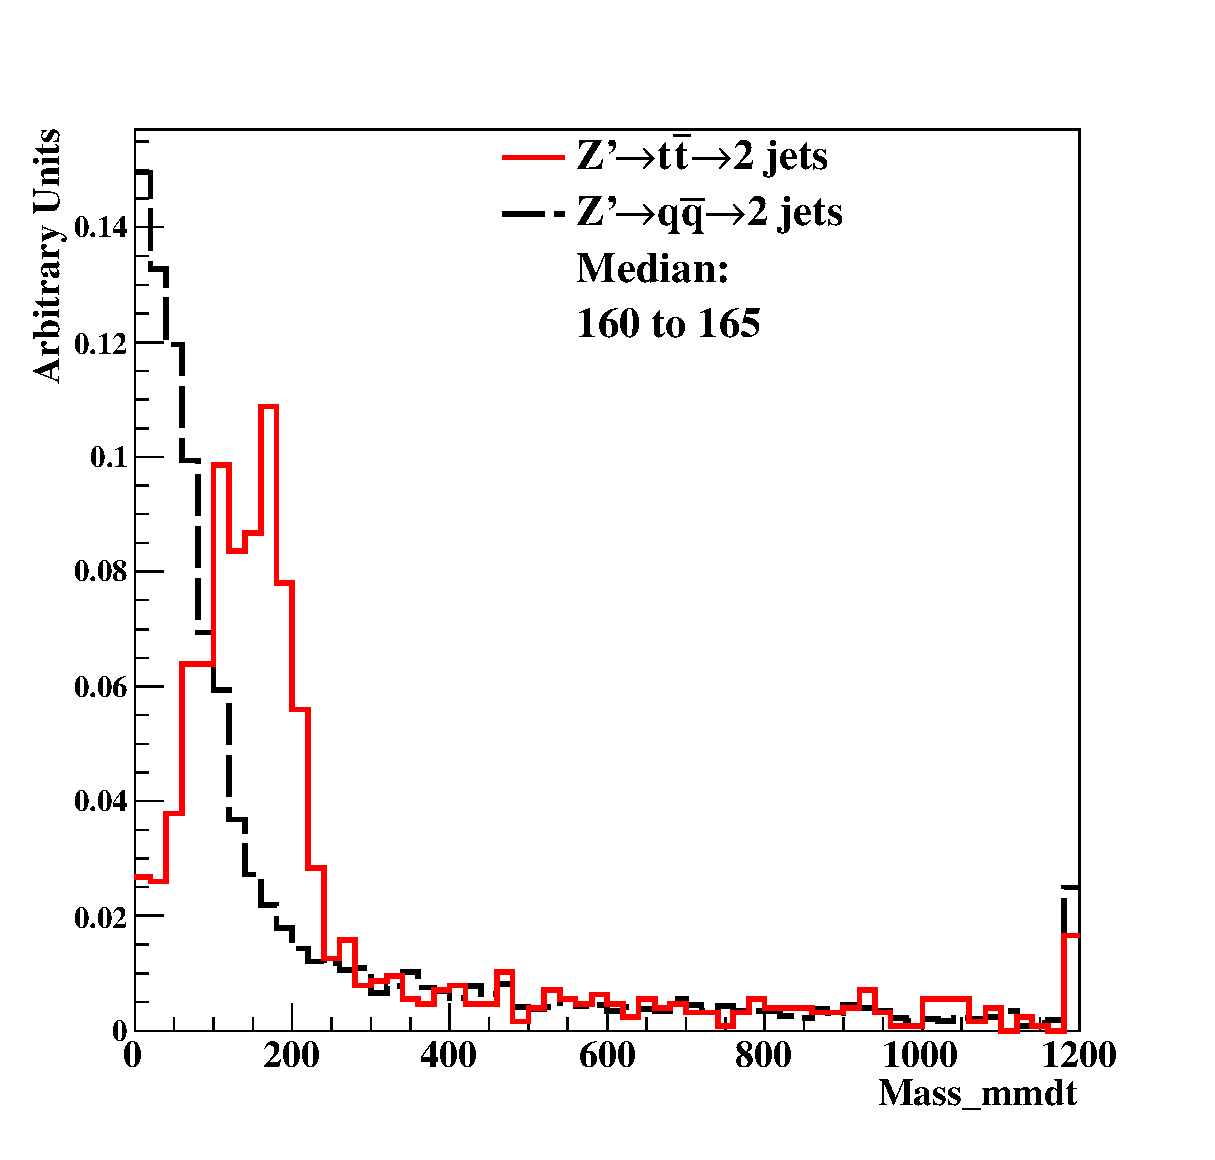
\includegraphics[   width=0.3\textwidth]{h_soft_drop/Dis_cluster_012_mass_mmdt_tt_20tev_04_tt_no_UOF.eps}\hfill
   }
\end{center}
\caption{
Distributions of soft drop mass for $\beta$=0, with 20 TeV c.m. energies and three different detector cell sizes: 20$\times$20, 
5$\times$5, and 1$\times$1 ($cm^2$). The signal (background) process is 
Z'$\rightarrow$t$\bar{\mathrm{t}}$ (Z'$\rightarrow$q$\bar{\mathrm{q}}$).
}
\label{fig:cluster_mass_mmdt_tt}
\end{figure}


\begin{figure}
\begin{center}
  \subfigure[Z'(5 TeV)] {
  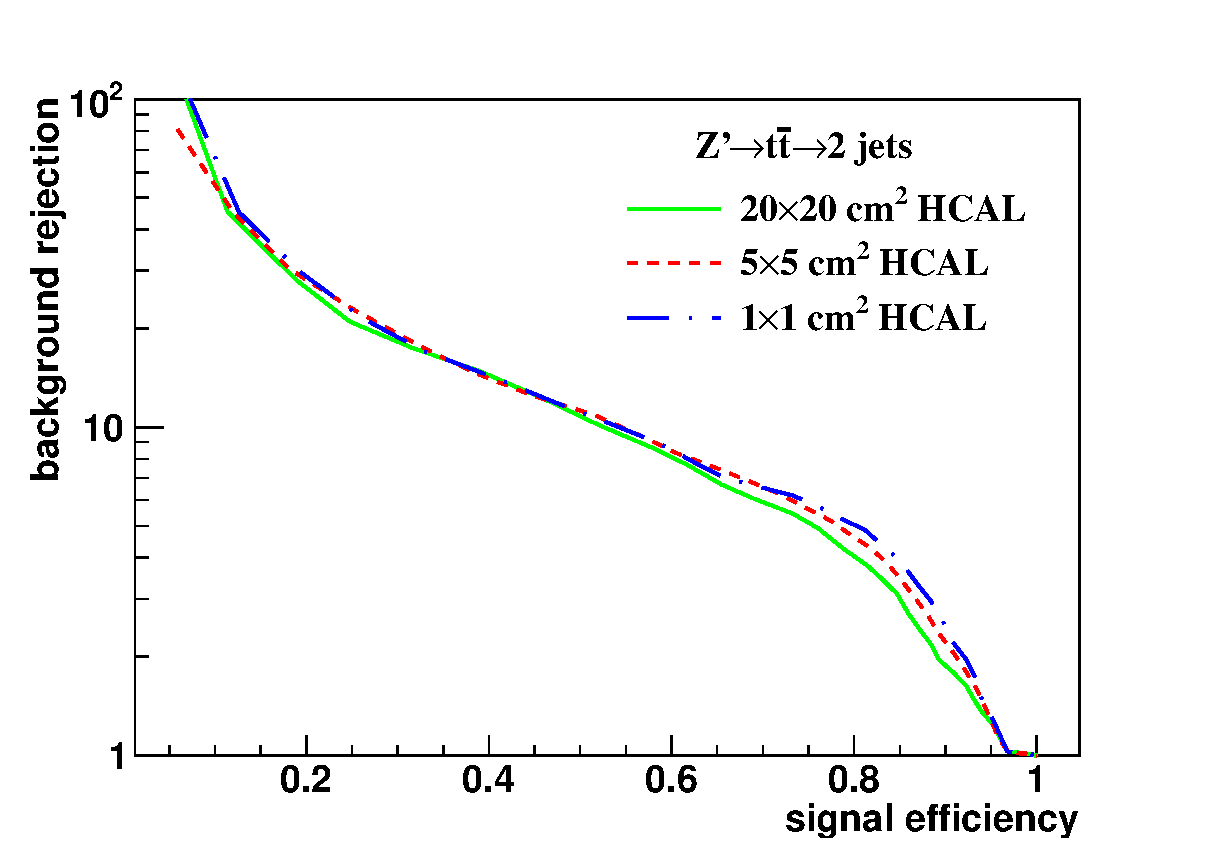
\includegraphics[  width=0.45\textwidth]{ROC_soft_drop/A_Cluster_mass_mmdt_5tev_eff_1_central_fix_at_Median_bin_tt_qq_log_no_UOF.eps}
  }
  \subfigure[Z'(10 TeV)] {
  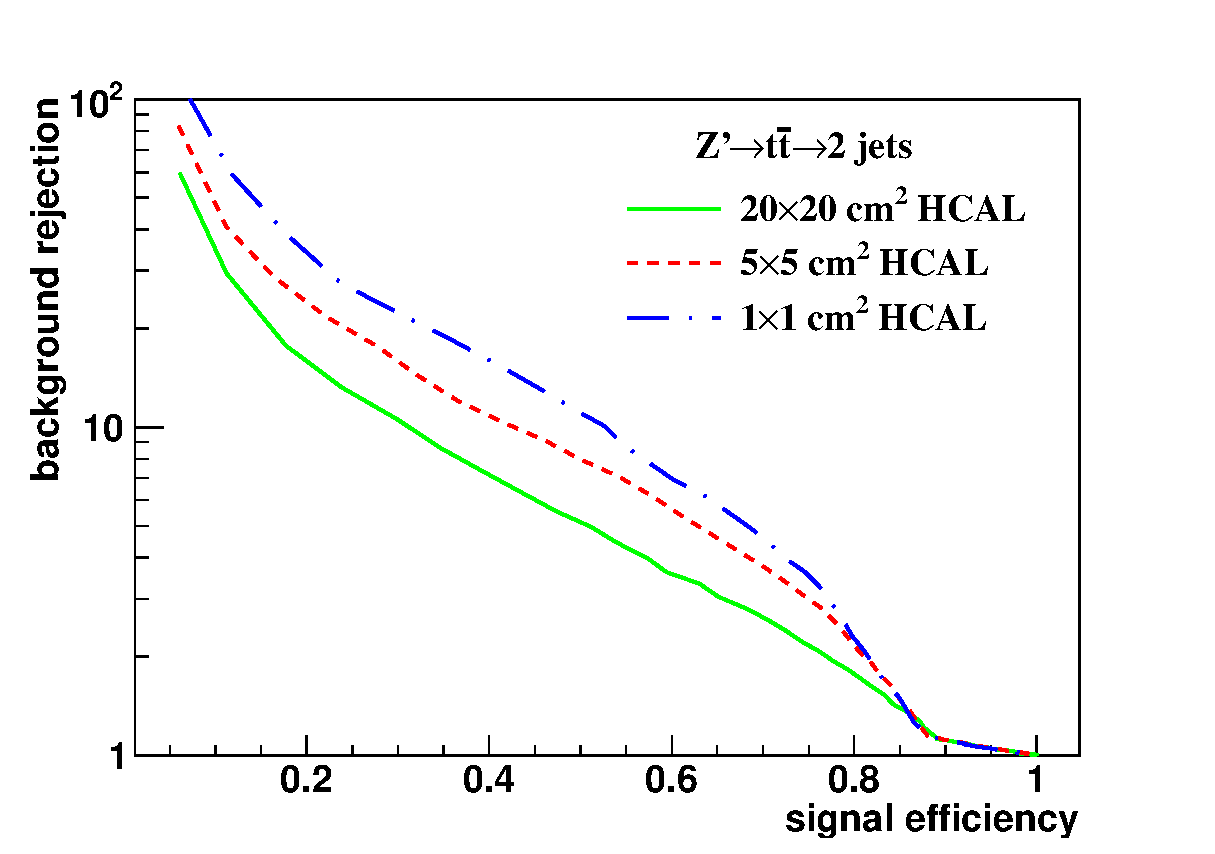
\includegraphics[  width=0.45\textwidth]{ROC_soft_drop/A_Cluster_mass_mmdt_10tev_eff_1_central_fix_at_Median_bin_tt_qq_log_no_UOF.eps}
  }
 \subfigure[Z'(20 TeV)] {
 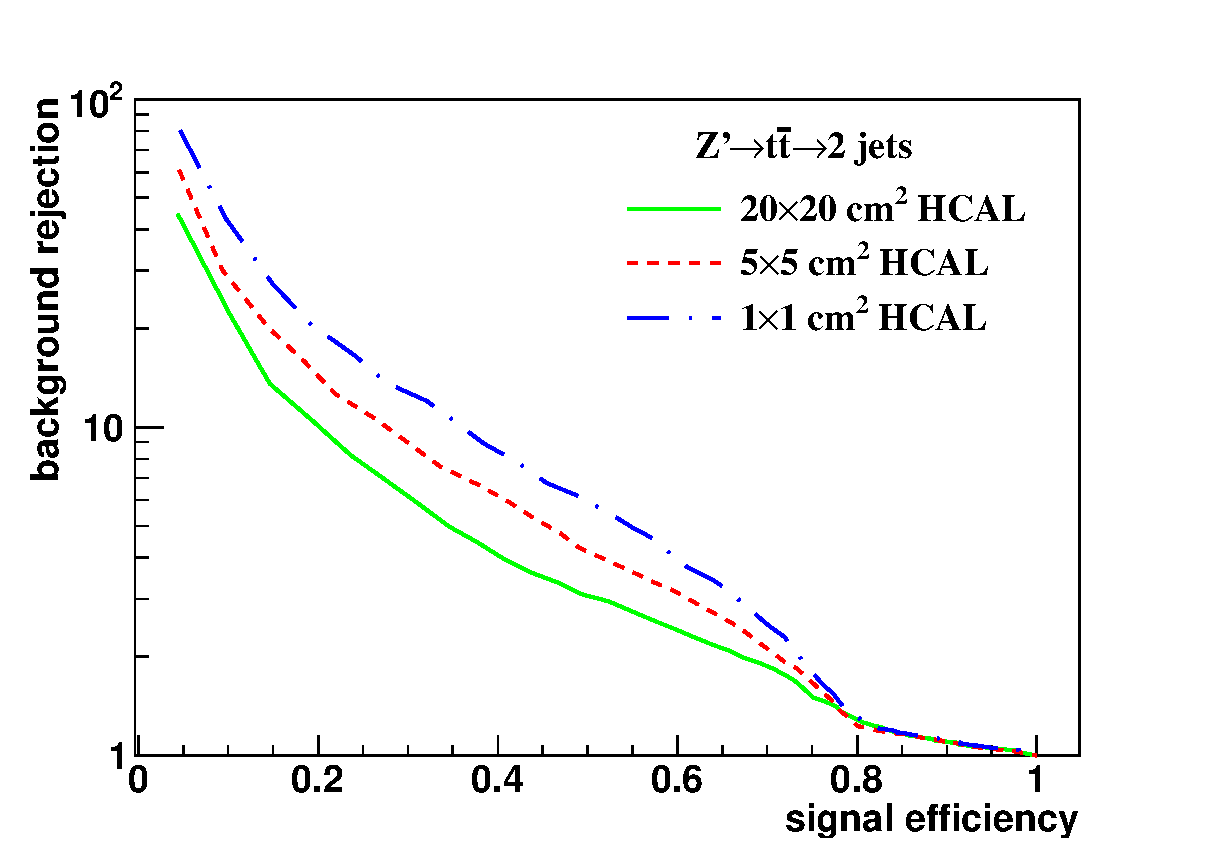
\includegraphics[  width=0.45\textwidth]{ROC_soft_drop/A_Cluster_mass_mmdt_20tev_eff_1_central_fix_at_Median_bin_tt_qq_log_no_UOF.eps}
 }
 \subfigure[Z'(40 TeV)] {
 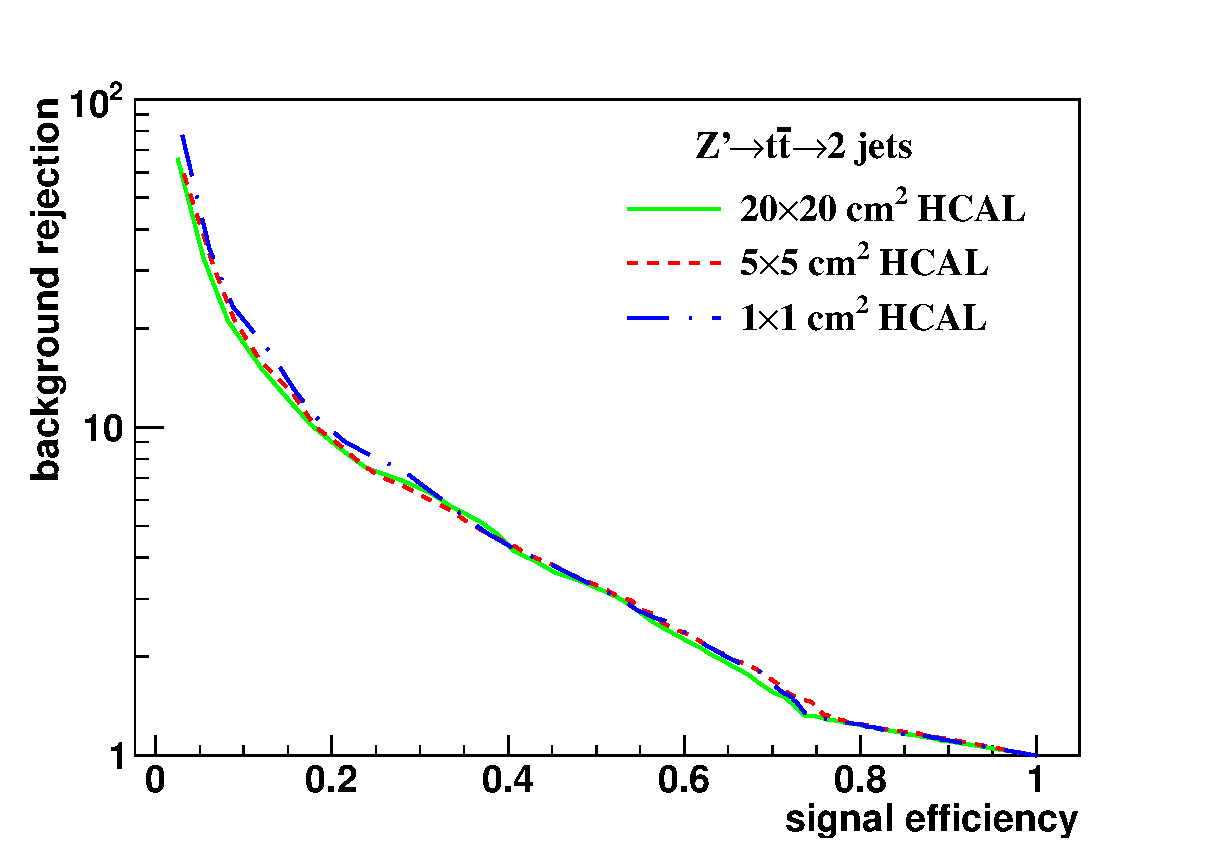
\includegraphics[  width=0.45\textwidth]{ROC_soft_drop/A_Cluster_mass_mmdt_40tev_eff_1_central_fix_at_Median_bin_tt_qq_log_no_UOF.eps}
 }
\end{center}
\caption{
The ROC curves of soft drop mass selection for $\beta$=0 
with 5,10, 20, 40 TeV c.m. energies. 
Three different detector cell sizes are compared: 20$\times$20, 
5$\times$5, and 1$\times$1 ($cm^2$). 
The signal (background) process is Z'$\rightarrow$t$\bar{\mathrm{t}}$
(Z'$\rightarrow$q$\bar{\mathrm{q}}$).
}
\label{fig:cluster_mass_mmdt_tt_ROC}
\end{figure}



\begin{figure}
\begin{center}
   \subfigure[20$\times$20 ($cm^2$)] {
   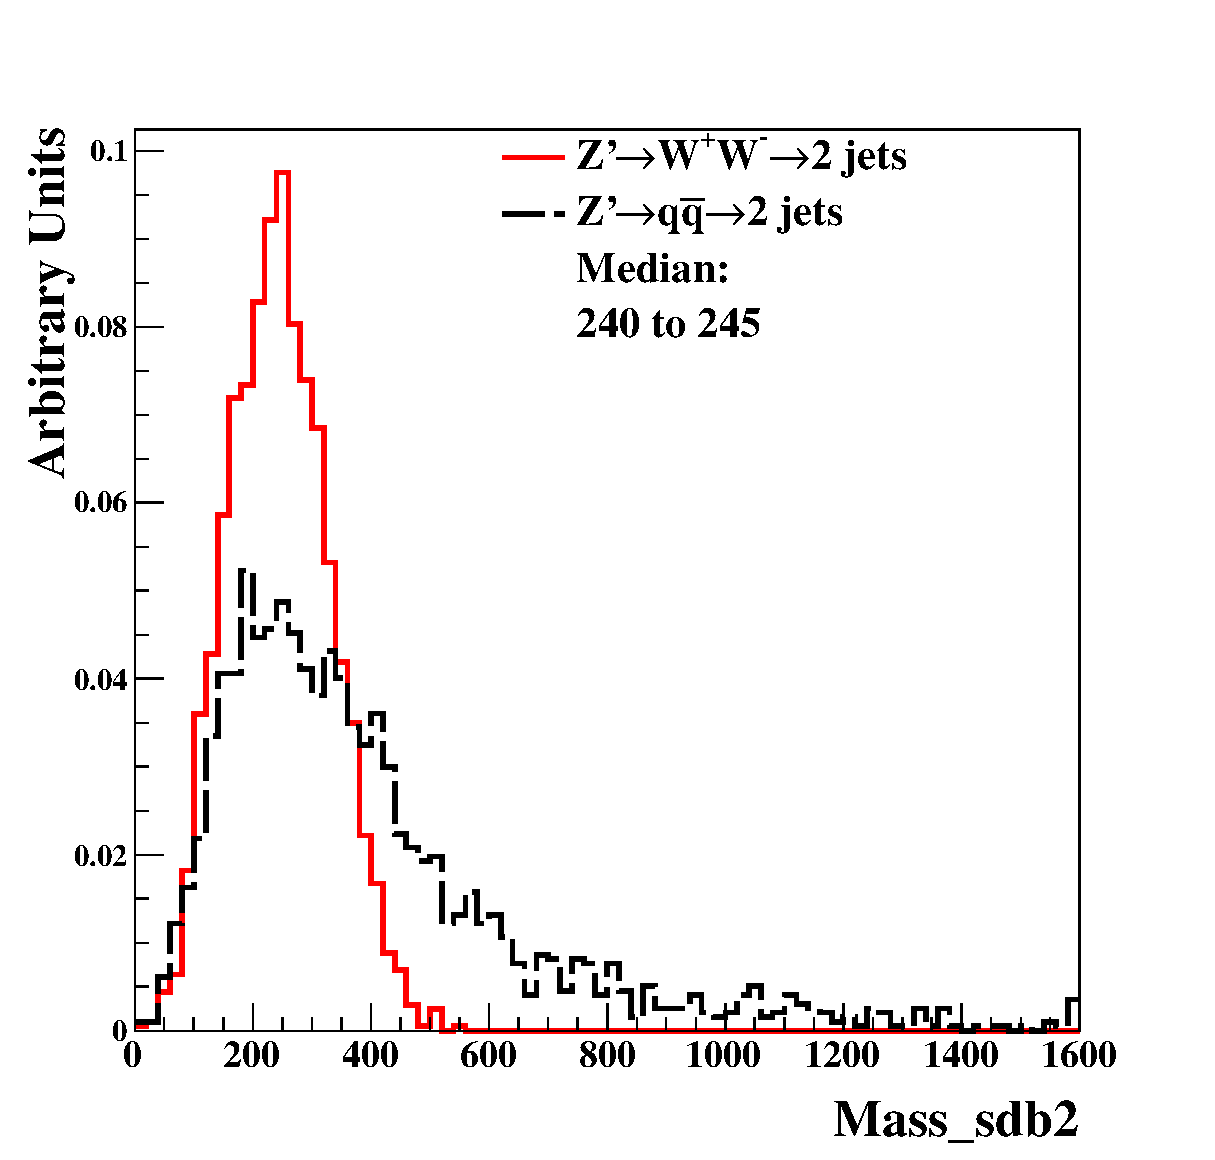
\includegraphics[   width=0.3\textwidth]{h_soft_drop/Dis_cluster_010_mass_sdb2_ww_20tev_04_1600_no_UOF.eps}
   }
    \subfigure[5$\times$5 ($cm^2$)] {
   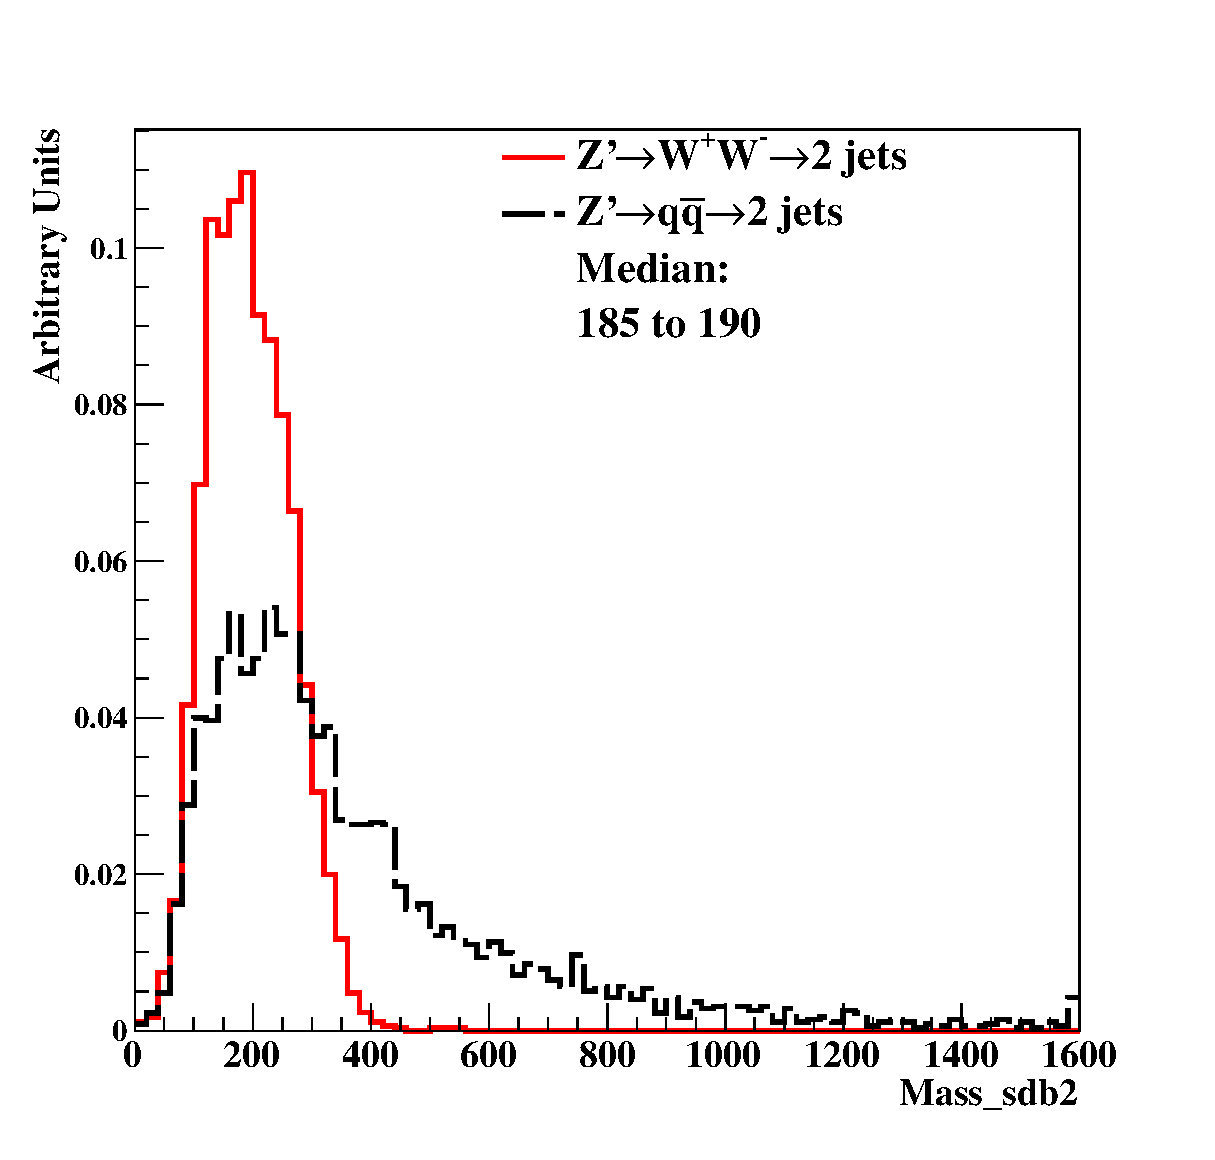
\includegraphics[   width=0.3\textwidth]{h_soft_drop/Dis_cluster_009_mass_sdb2_ww_20tev_04_1600_no_UOF.eps}\hfill
   }
   \subfigure[1$\times$1 ($cm^2$)] {
   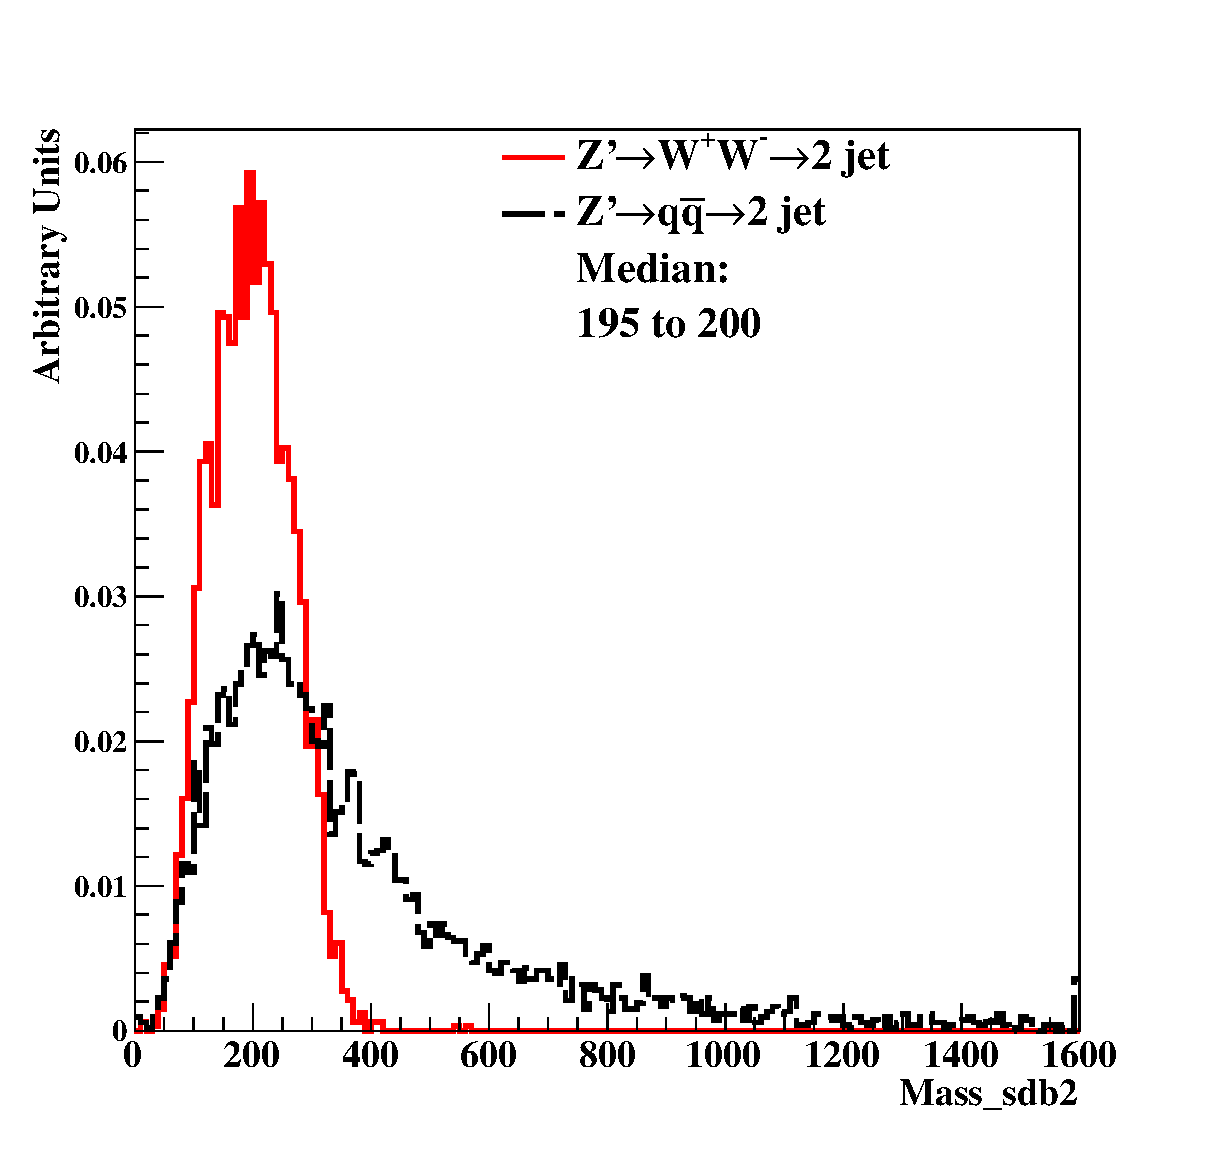
\includegraphics[   width=0.3\textwidth]{h_soft_drop/Dis_cluster_012_mass_sdb2_ww_20tev_04_1600_no_UOF.eps}\hfill
   }
\end{center}
\caption{
Distributions of soft drop mass for $\beta$=2, with 20 TeV c.m. energies and three different detector cell sizes: 20$\times$20, 
5$\times$5, and 1$\times$1 ($cm^2$). The signal (background) process is 
Z'$\rightarrow$WW (Z'$\rightarrow$q$\bar{\mathrm{q}}$).
}
\label{fig:cluster_mass_sdb2_ww}
\end{figure}


\begin{figure}
\begin{center}
  \subfigure[Z'(5 TeV)] {
  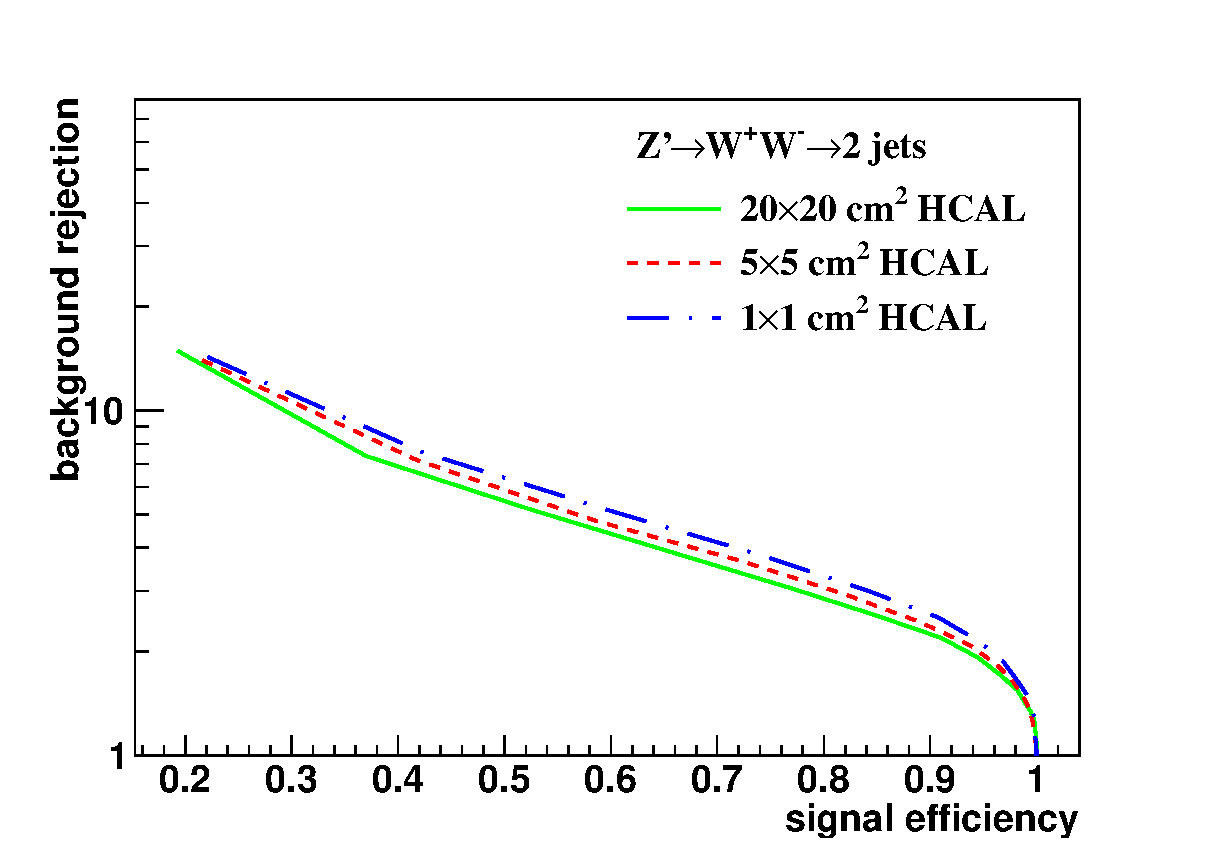
\includegraphics[  width=0.45\textwidth]{ROC_soft_drop/A_Cluster_mass_sdb2_5tev_eff_1_central_fix_at_Median_bin_ww_qq_log_no_UOF.eps}
  }
  \subfigure[Z'(10 TeV)] {
  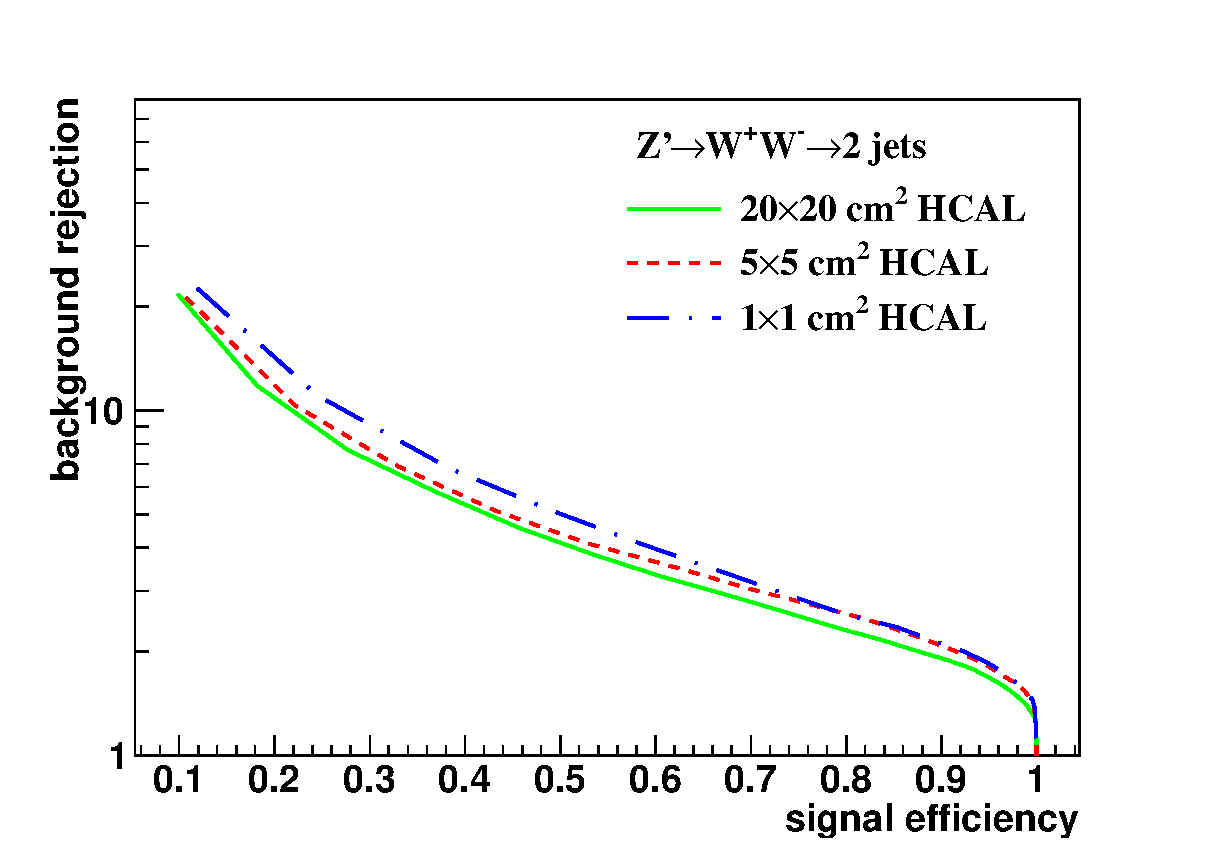
\includegraphics[  width=0.45\textwidth]{ROC_soft_drop/A_Cluster_mass_sdb2_10tev_eff_1_central_fix_at_Median_bin_ww_qq_log_no_UOF.eps}
  }
 \subfigure[Z'(20 TeV)] {
 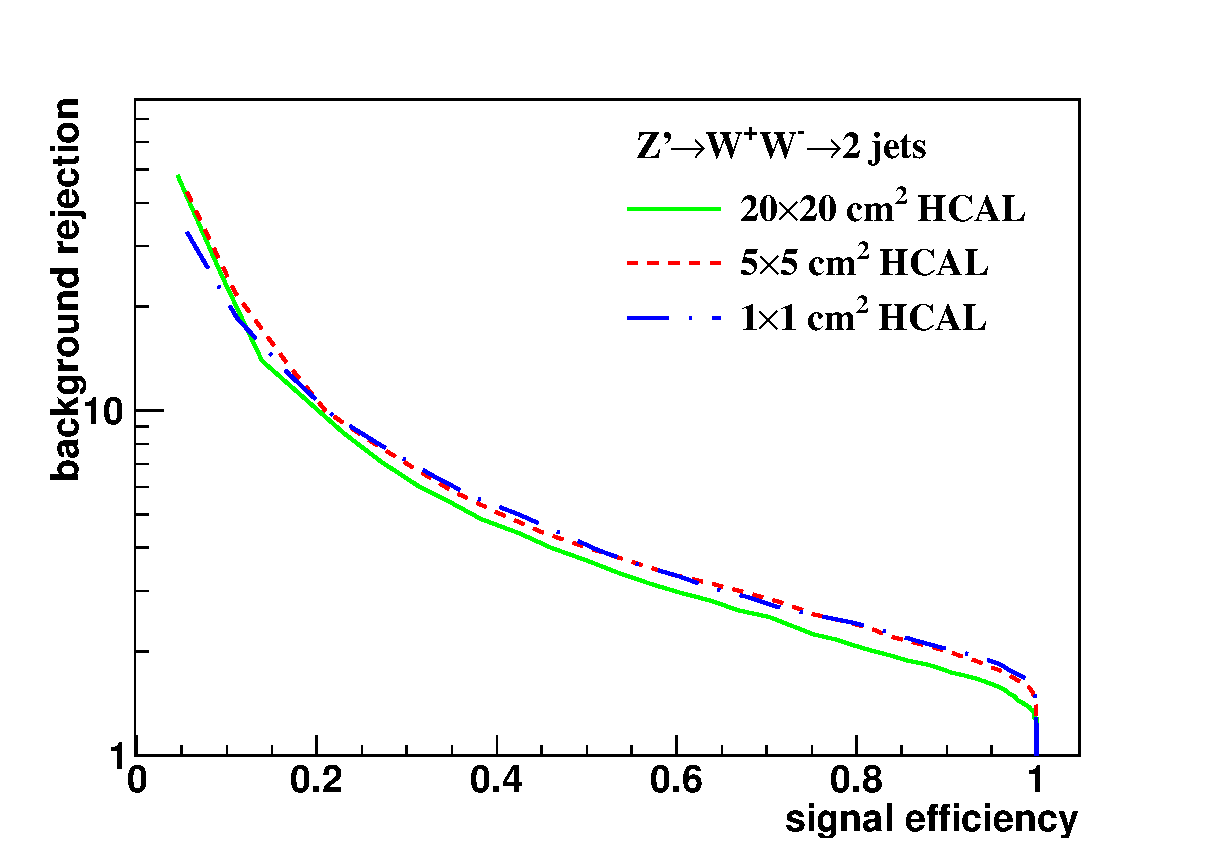
\includegraphics[  width=0.45\textwidth]{ROC_soft_drop/A_Cluster_mass_sdb2_20tev_eff_1_central_fix_at_Median_bin_ww_qq_log_no_UOF.eps}
 }
 \subfigure[Z'(40 TeV)] {
 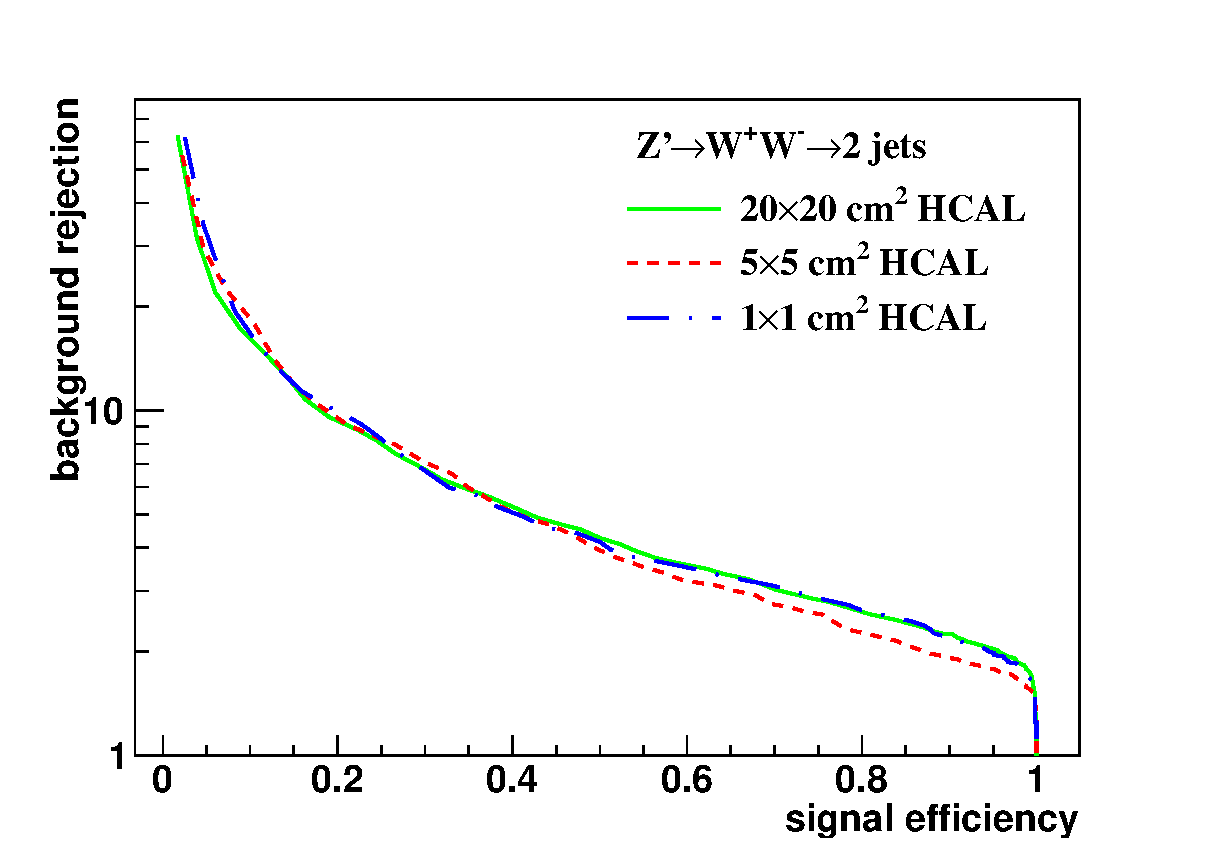
\includegraphics[  width=0.45\textwidth]{ROC_soft_drop/A_Cluster_mass_sdb2_40tev_eff_1_central_fix_at_Median_bin_ww_qq_log_no_UOF.eps}
 }
\end{center}
\caption{
The ROC curves of soft drop mass selection for $\beta$=2
with 5, 10, 20, 40 TeV c.m. energies. 
Three different detector cell sizes are compared: 20$\times$20, 
5$\times$5, and 1$\times$1 ($cm^2$). 
The signal (background) process is Z'$\rightarrow$WW 
(Z'$\rightarrow$q$\bar{\mathrm{q}}$).
}
\label{fig:cluster_mass_sdb2_ww_ROC}
\end{figure}


\begin{figure}
\begin{center}
   \subfigure[20$\times$20 ($cm^2$)] {
   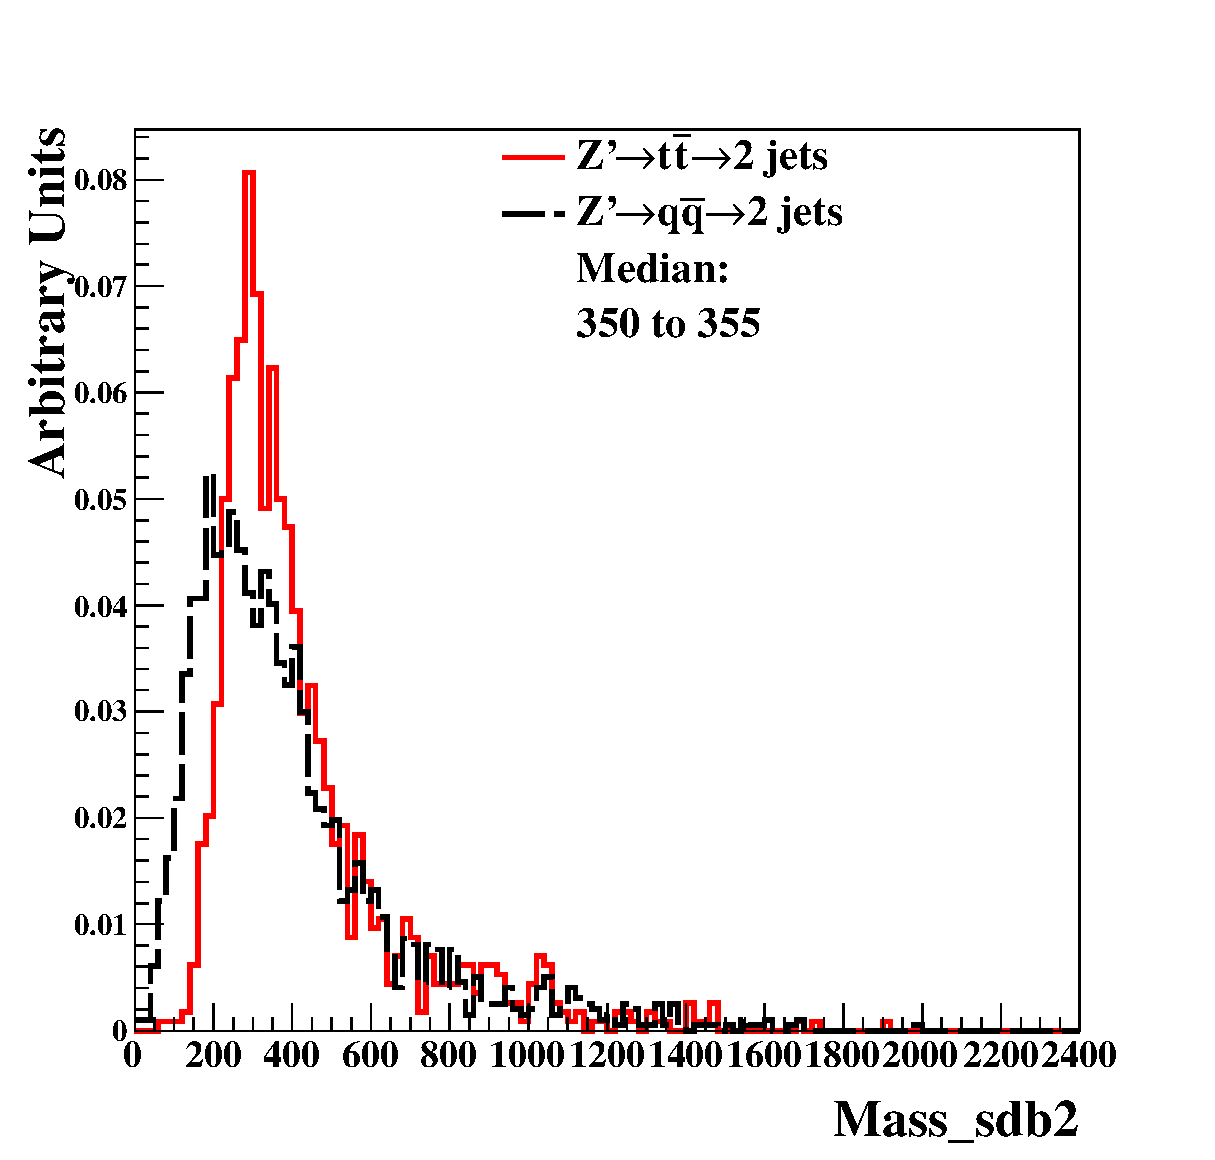
\includegraphics[   width=0.3\textwidth]{h_soft_drop/Dis_cluster_010_mass_sdb2_tt_20tev_04_tt_2400_no_UOF.eps}
   }
   \subfigure[5$\times$5 ($cm^2$)] {
   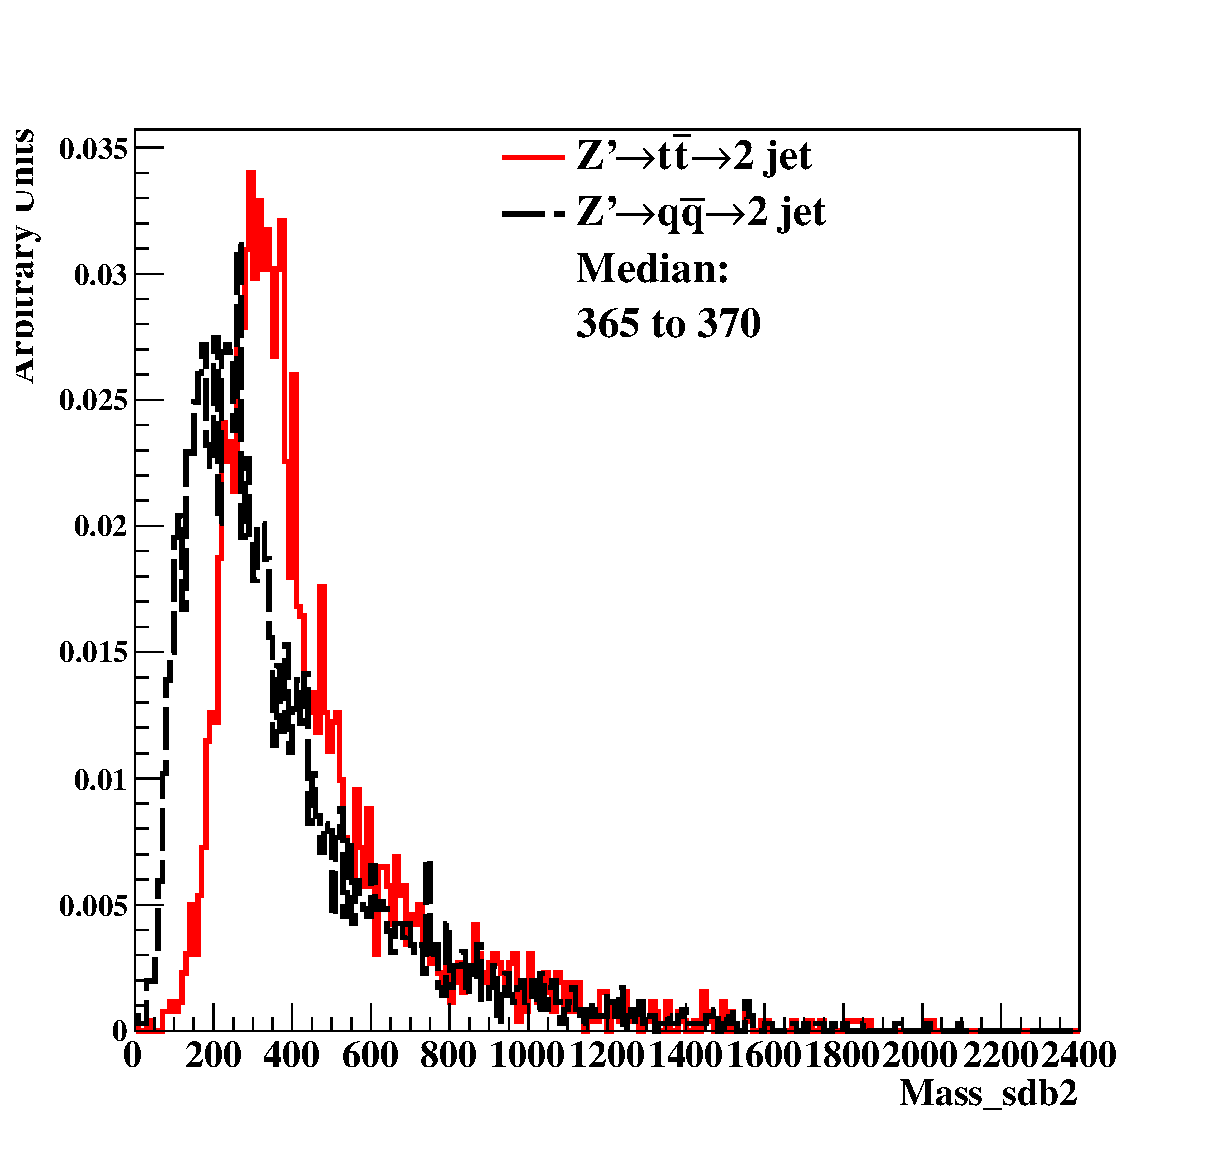
\includegraphics[   width=0.3\textwidth]{h_soft_drop/Dis_cluster_009_mass_sdb2_tt_20tev_04_tt_2400_no_UOF.eps}\hfill
   }
   \subfigure[1$\times$1 ($cm^2$)] {
   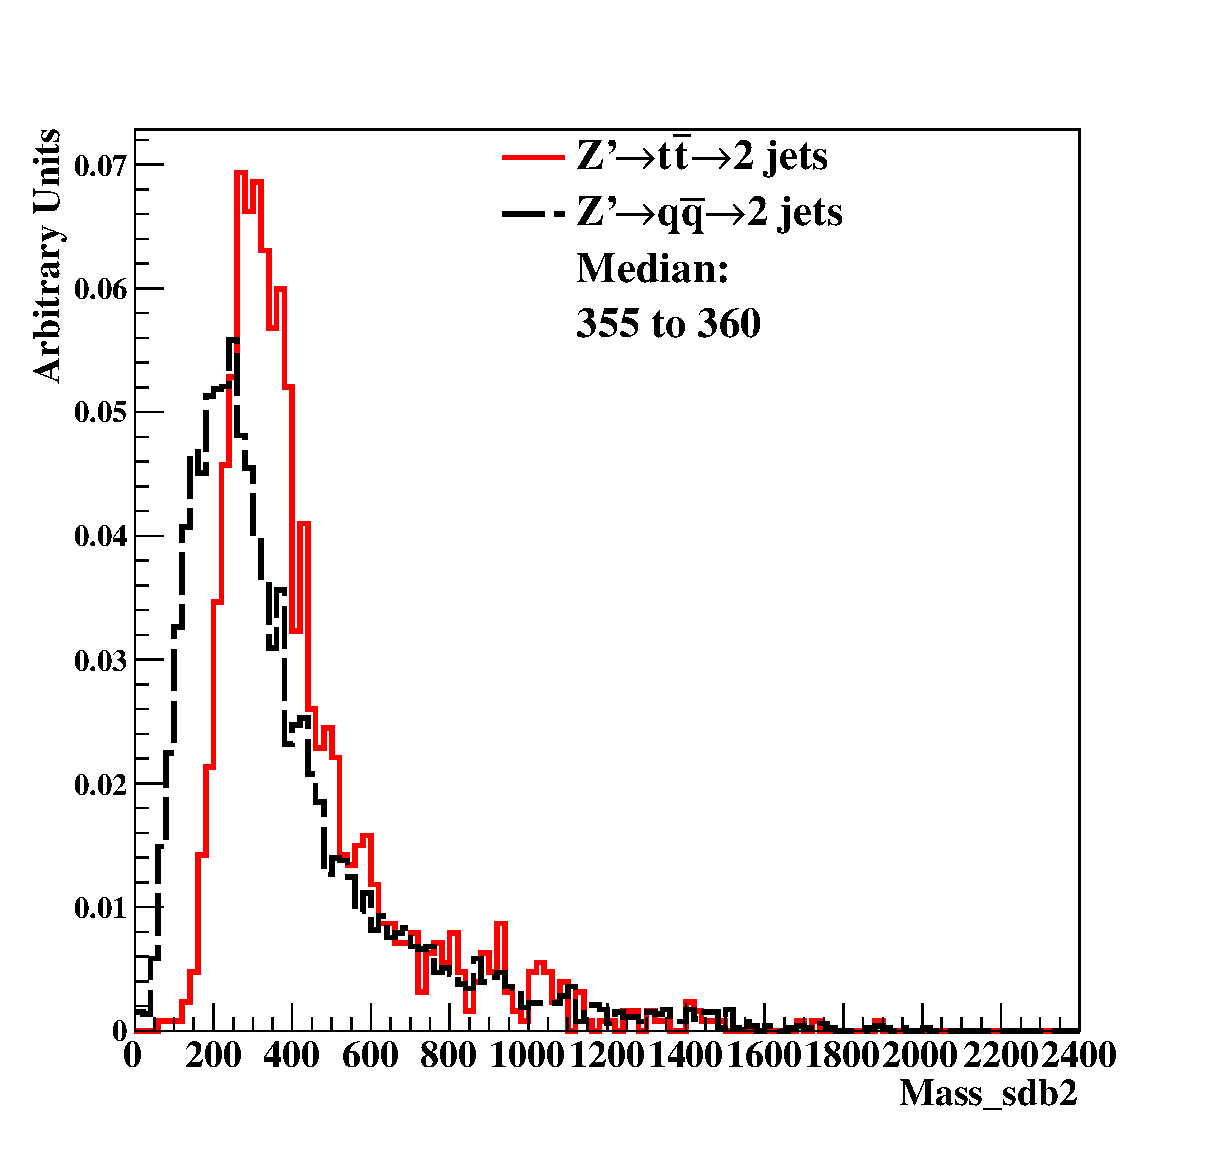
\includegraphics[   width=0.3\textwidth]{h_soft_drop/Dis_cluster_012_mass_sdb2_tt_20tev_04_tt_2400_no_UOF.eps}\hfill
   }
\end{center}
\caption{
Distributions of soft drop mass for $\beta$=2, with 20 TeV c.m. energies and three different detector cell sizes: 20$\times$20, 
5$\times$5, and 1$\times$1 ($cm^2$). The signal (background) process is 
Z'$\rightarrow$t$\bar{\mathrm{t}}$ (Z'$\rightarrow$q$\bar{\mathrm{q}}$).
}
\label{fig:cluster_mass_sdb2_tt}
\end{figure}


\begin{figure}
\begin{center}
  \subfigure[Z'(5 TeV)] {
  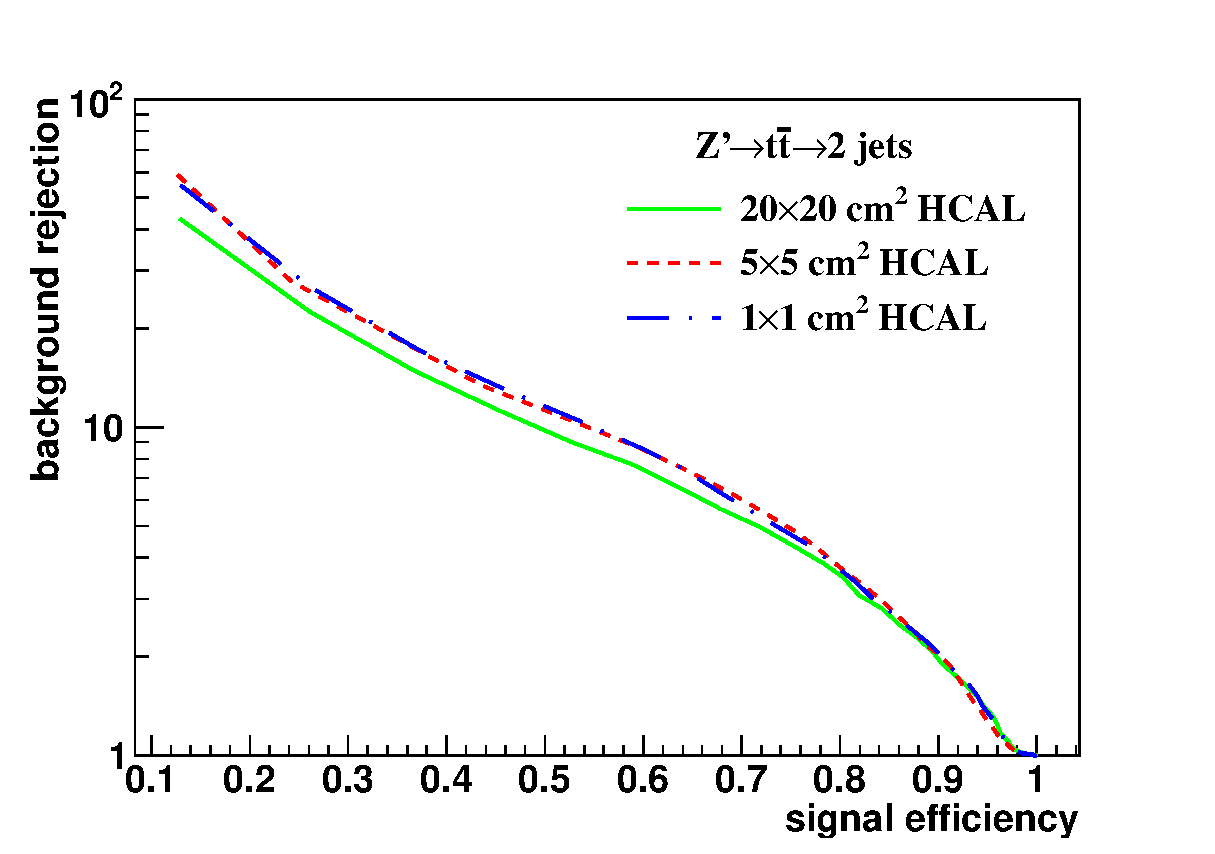
\includegraphics[  width=0.45\textwidth]{ROC_soft_drop/A_Cluster_mass_sdb2_5tev_eff_1_central_fix_at_Median_bin_tt_qq_log_no_UOF.eps}
  }
  \subfigure[Z'(10 TeV)] {
  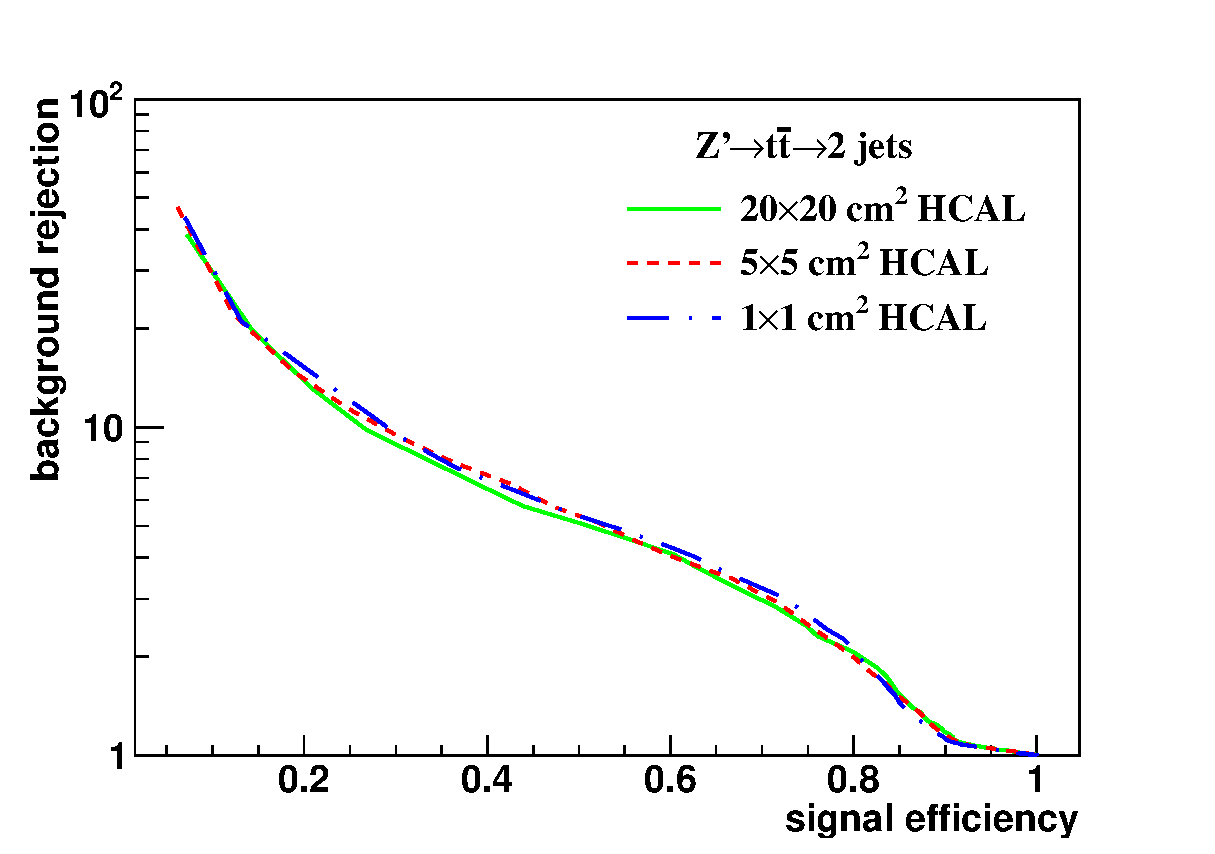
\includegraphics[  width=0.45\textwidth]{ROC_soft_drop/A_Cluster_mass_sdb2_10tev_eff_1_central_fix_at_Median_bin_tt_qq_log_no_UOF.eps}
  }
 \subfigure[Z'(20 TeV)] {
 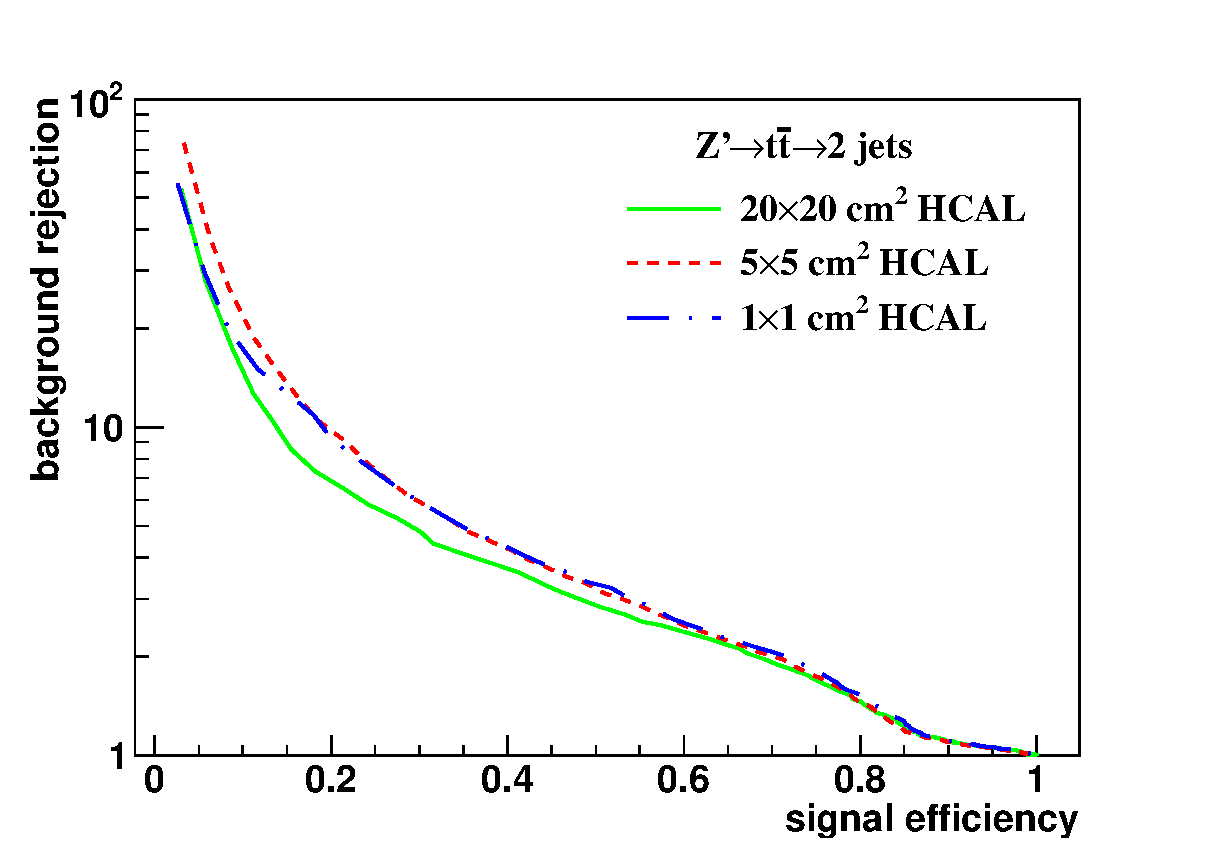
\includegraphics[  width=0.45\textwidth]{ROC_soft_drop/A_Cluster_mass_sdb2_20tev_eff_1_central_fix_at_Median_bin_tt_qq_log_no_UOF.eps}
 }
 \subfigure[Z'(40 TeV)] {
 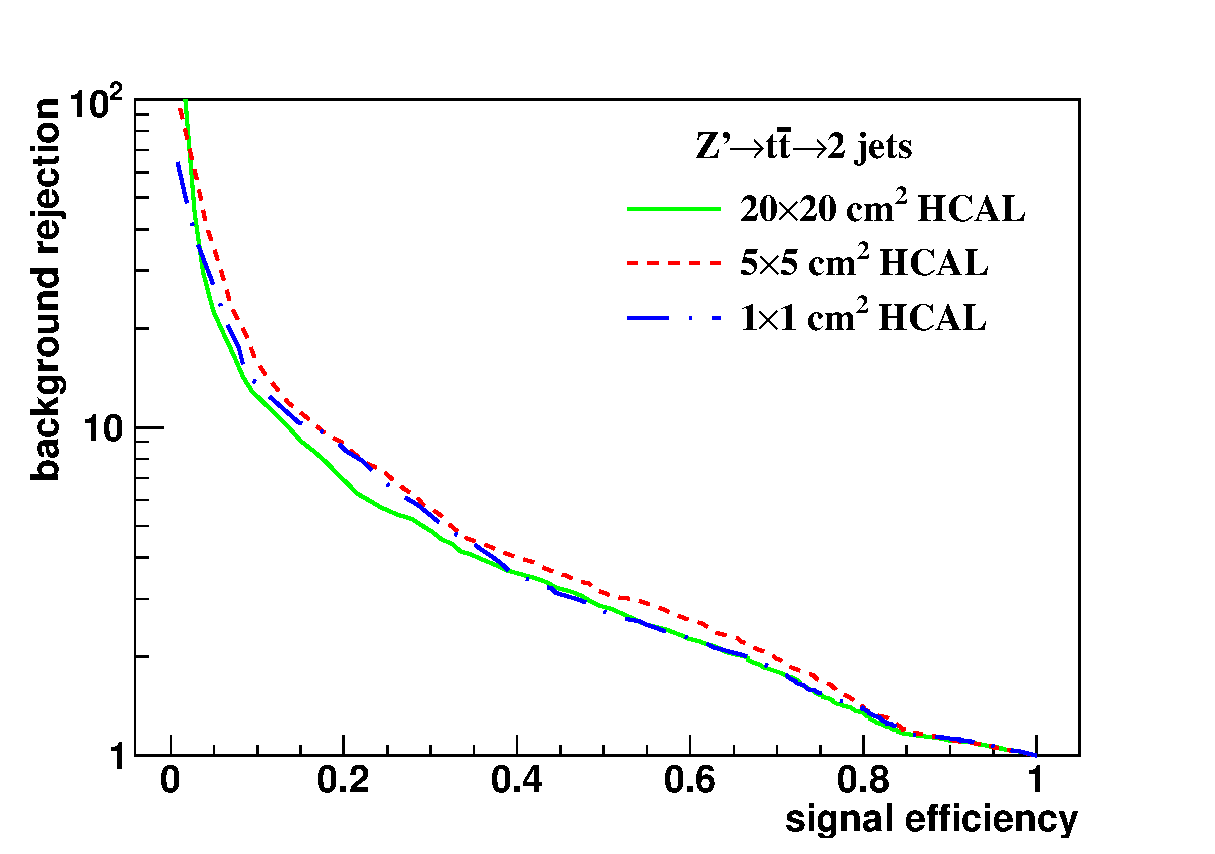
\includegraphics[  width=0.45\textwidth]{ROC_soft_drop/A_Cluster_mass_sdb2_40tev_eff_1_central_fix_at_Median_bin_tt_qq_log_no_UOF.eps}
 }
\end{center}
\caption{
The ROC curves of soft drop mass selection for $\beta$=2
with 5, 10, 20, 40 TeV c.m. energies. 
Three different detector cell sizes are compared: 20$\times$20, 
5$\times$5, and 1$\times$1 ($cm^2$). 
The signal (background) process is Z'$\rightarrow$t$\bar{\mathrm{t}}$
(Z'$\rightarrow$q$\bar{\mathrm{q}}$).
}
\label{fig:cluster_mass_sdb2_tt_ROC}
\end{figure}






\section{Study of detector performance with jet substructure variables}
In this section, we use several jet substructure variables to study the performance of detector with various detector cell sizes and c.m. energies.
%%By definition of Mann Whitney U test, if U value is close to 0.5, it means two distributions have similar compositions, and we can not distinguish them very well. On the other hand, if U value of two distributions are close to 0, it means both compositions of both distribution are much different from each other.\\

\subsection{$N$-subjettiness \label{sec:nsub}}
The variable $N$-subjettiness~\cite{Thaler:2010tr}, denoted by $\tau_N$, is designed to 
``count'' the number of subjet(s) in a large radius jet so to separate 
signal jets from decays of heavy bosons and background jets from QCD processes. 
The $\tau_N$ is the $\pt$-weighted angular distance between each jet 
constituent and the closest subjet axis: 
\begin{equation}\label{eq:Nsub_1}
\tau_{N}=\frac{1}{d_{0}}\sum_{k}p_{T,k} \mathrm{min}\{\Delta R_{1,k},\Delta R_{2,k},.....\Delta R_{N,k}\},
\end{equation}
with a normalization factor $d_0$: \[d_{0}=\sum_{k}p_{T,k} R_{0}.\] 
The $k$ runs over all constituent particles in a given large radius jet, 
$p_{T,k}$ is the transverse momentum of each individual constituent particle, 
$\Delta R_{j,k}=\sqrt{(\Delta y)^{2}+(\Delta \phi)^{2}}$ is the distance 
between the constituent particle $k$ and the candidate subjet axis $j$ in the 
$y-\phi$ plane. The $R_{0}$ is the characteristic jet radius used in 
the anti-$k_t$ jet algorithm. 

In this analysis, the anti-$k_t$ algorithm with $R=0.4$ (AK4) is first 
employed to reconstruct jets. The subjet axes are obtained by running the 
exclusive $k_{t}$ algorithm~\cite{Catani:246812} and reversing the last N clustering steps. 
Namely, when $\tau_N$ is computed, the $k_{t}$ algorithm is forced to return 
exactly $N$ jets. If a large radius jet has $N$ subjet(s), its $\tau_{N}$ is 
smaller than $\tau_{N-1}$. Therefore, in our analysis, 
the ratio of the $\tau_{N}$ variables, 
$\tau_{21}$ ($\tau_{2}/\tau_{1}$) and $\tau_{32}$ ($\tau_{3}/\tau_{2}$),  
are used to distinguish the one-prong background jets and 
the two-prong jets from W or the three-prong jets from top. 

We use the ROC curves as described in Section~\ref{sec:massana} to 
analyze the detector performance and determine the cell size that gives the 
best separation power to distinguish signal from background. 
Following the suggestion by Ref.~\cite{Dreyer:2018tjj}, requirement on the 
soft drop mass with $\beta=0$ is applied before the study of $N$-subjettiness. 
For each detector configuration and c.m. energy, the soft drop mass selection 
is determined as follows. First, we look for the median bin of the soft drop 
mass histogram from simulated signal events as described in 
Section~\ref{sec:massana}.  Then, we compare the numbers of events in the 
bins adjacent to the medium bin (bin $i_\mathrm{med}-1$ 
and bin $i_\mathrm{med}+1$). The bin with larger number of events is added, 
in addition to the medium bin, to extend the mass window. The procedure is 
repeated until the window contains at least 75\% of the total number of signal 
events. 

In order to obtain the signal and background efficiencies, 
various ranges of the $\tau_{21}$ and $\tau_{32}$ are scanned. 
Since some of the background distributions have long tails and leak into the 
signal-dominated region, we use the following method as suggested by the 
Pearson Lemma Method~\cite{} to determine the ranges of $\tau$ variables. 
First, we take the ratio of the signal to background $\tau_{21}$ ($\tau_{32}$) 
histograms. The boundaries of the bin (seed bin) with maximum signal to 
background ratio (S/N) give us the first range of $\tau$ selection: 
$x_\mathrm{low}^\mathrm{seedbin} < \tau_{21} <  x_\mathrm{high}^\mathrm{seedbin}$. 
Then, we compare the S/N in the bins adjacent to the seed bin. The bin with 
larger S/N is added, in addition to the seed bin, to extend the $\tau_{21}$ 
selection window. 
Every window has its corresponding $\epsilon_\mathrm{sig}$ and 
1/$\epsilon_\mathrm{bkg}$ and an ROC curve is mapped out. 

In addition to the ROC curves, we use the so-called "Mann-Whitney" test to 
quantify the detector performance. 
The value of Mann-Whitney is related to the integrated area under the ROC 
curve: if the value is bigger, it indicates the signal and background
 distributions have similar shapes and can not be well separated from 
each other. Vice versa, if the value is smaller, we can achieve a better 
signal and background separation. 

%First, we select the events in mass window by using SD with $\beta=0$ and 75$\%$ signal efficiency. Then, we find the highest ratio bin to be our seed bin. Next, we compare the left and right of ratio bin, and add the higher bin to be our width. Finally,  We can use this width to draw the ROC curves.\\
Figures~\ref{fig:Rawhit_05GeV_tau21_Dis} and~\ref{fig:Rawhit_05GeV_tau32_Dis} 
show the distributions of $\tau_{21}$ and $\tau_{32}$ for $\sqrt{s}=20$~TeV 
after applying requirement on the soft drop mass. The signals considered are 
Z'$\rightarrow$WW ($\tau_{21}$) and 
Z'$\rightarrow\mathrm{t}\bar{\mathrm{t}}$ ($\tau_{32}$). 
Figures~\ref{fig:Rawhit_05GeV_tau21_ROC} and~\ref{fig:Rawhit_05GeV_tau32_ROC} 
present the ROC curves from different detector cell sizes and c.m. energies, 
respectively. The smallest detector cell size ($1\times1~\mathrm{cm}^2$) 
does not have the best separation power. In fact, in some cases, 
the best separation power comes from detector with bigger cell sizes 
($5\times5~\mathrm{cm}^2$ and $20\times20~\mathrm{cm}^2$).

Figures~\ref{fig:Rawhit_05GeV_total_Mann} (a) and (b) present the summary plots of $\tau_{21}$ and $\tau_{32}$ with various detector cell sizes and c.m. energies using Mann Whitney U test. For $\tau_{21}$ at smaller c.m. energies, when 
cell size is smaller, the detector performance improves. However, 
when c.m. energy increases, no improvement 
is observed using the smallest detector cell size ($1\times1~\mathrm{cm}^2$). 
For $\tau_{32}$, the case is similar to  $\tau_{21}$. Even worse, with some 
c.m. energies, the bigger detector cell sizes ($5\times5~\mathrm{cm}^2$ and $20\times20~\mathrm{cm}^2$) have better separation power than the smallest 
detector size. 

\subsection{Energy correlation function \label{sec:ecf}}
The energy correlation function (ECF)~\cite{Larkoski:2013eya} is defined as follows: 
%\begin{equation} \label{eq:ECF_Original}
%ECF(N,\beta)=\sum_{i_{1}<i_{2}<....<i_{N}\in J} (\prod_{a=1}^{N}E_{ia})(\prod_{%b=1}^{N-1}\prod_{c=b+1}^{N} \theta_{i_{b}i_{c}})^{\beta}, 
%\end{equation}
\begin{equation} \label{eq:ECF_Modified}
ECF(N,\beta)=\sum_{i_{1}<i_{2}<....<i_{N}\in J} \left(\prod_{a=1}^{N}p_{\mathrm{T}ia}\right)\left(\prod_{b=1}^{N-1}\prod_{c=b+1}^{N} R_{i_{b}i_{c}}\right)^{\beta},
\end{equation}
where the sum is looped all particles in the jet $J$, $\pt$ is the transverse 
momentum of each individual particle, and $R$ is the distance between two 
particles in the $y$-$\phi$ plane.  
In order to use a dimensionless variable, a parameter $r_{N}$ is defined:
\begin{equation} \label{eq:ECF_ratio}
r_{N}^{(\beta)}\equiv\frac{ECF(N+1,\beta)}{ECF(N,\beta)}.
\end{equation}

The idea of $r_N$ comes from N-subjettiness $\tau_N$. Both $r_N$ and $\tau_N$ 
are linear in the energy of the soft radiation for a system of $N$ partons 
with soft radiation. In general, if the system has N subjets, $ECF(N+1,\beta)$ 
should be significantly smaller than $ECF(N,\beta)$. Therefore, we can use this
 feature to distinguish jets with different number of subjets. 
As in Section~\ref{sec:nsub}, the ratio $r_N/r_{N-1}$, denoted by $C_N$, 
(double ratios of ECFs) is used to study the detector performance: 
\begin{equation}
C_{N}^{(\beta)}\equiv\frac{r_{N}^{(\beta)}}{r_{N-1}^{(\beta)}}=\frac{ECF(N-1,\beta)ECF(N+1,\beta)}{ECF(N,\beta)^2}.
\end{equation}
In our analysis, we set $N=2$ and $\beta=1$ ($C_2^1$).

Figure~\ref{fig:Rawhit_05GeV_c2b1_Dis} presents the histograms of $C_{2}^{1}$ 
with $\sqrt{s}=20$~TeV after making requirement on the soft drop mass. 
The signal considered is Z'$\rightarrow$WW. 
Figure~\ref{fig:Rawhit_05GeV_c2b1_ROC} shows the ROC curves from different 
detector cell sizes for each c.m. energy, respectively. One can see that 
the smallest detector cell size ($1\times1~\mathrm{cm}^2$) does not have the 
best signal/background separation power. 
Figure \ref{fig:Rawhit_05GeV_total_Mann}(c) summarizes the result of 
the Mann Whitney U test for $C_{2}^{1}$. When c.m. energy increases, 
no improvement is observed from detector with the smallest cell size. 


%%%%%%%%%%%% tau21
%25bins
\begin{figure}
\begin{center}
   \subfigure[20$\times$20 (cm$^2$)] {
   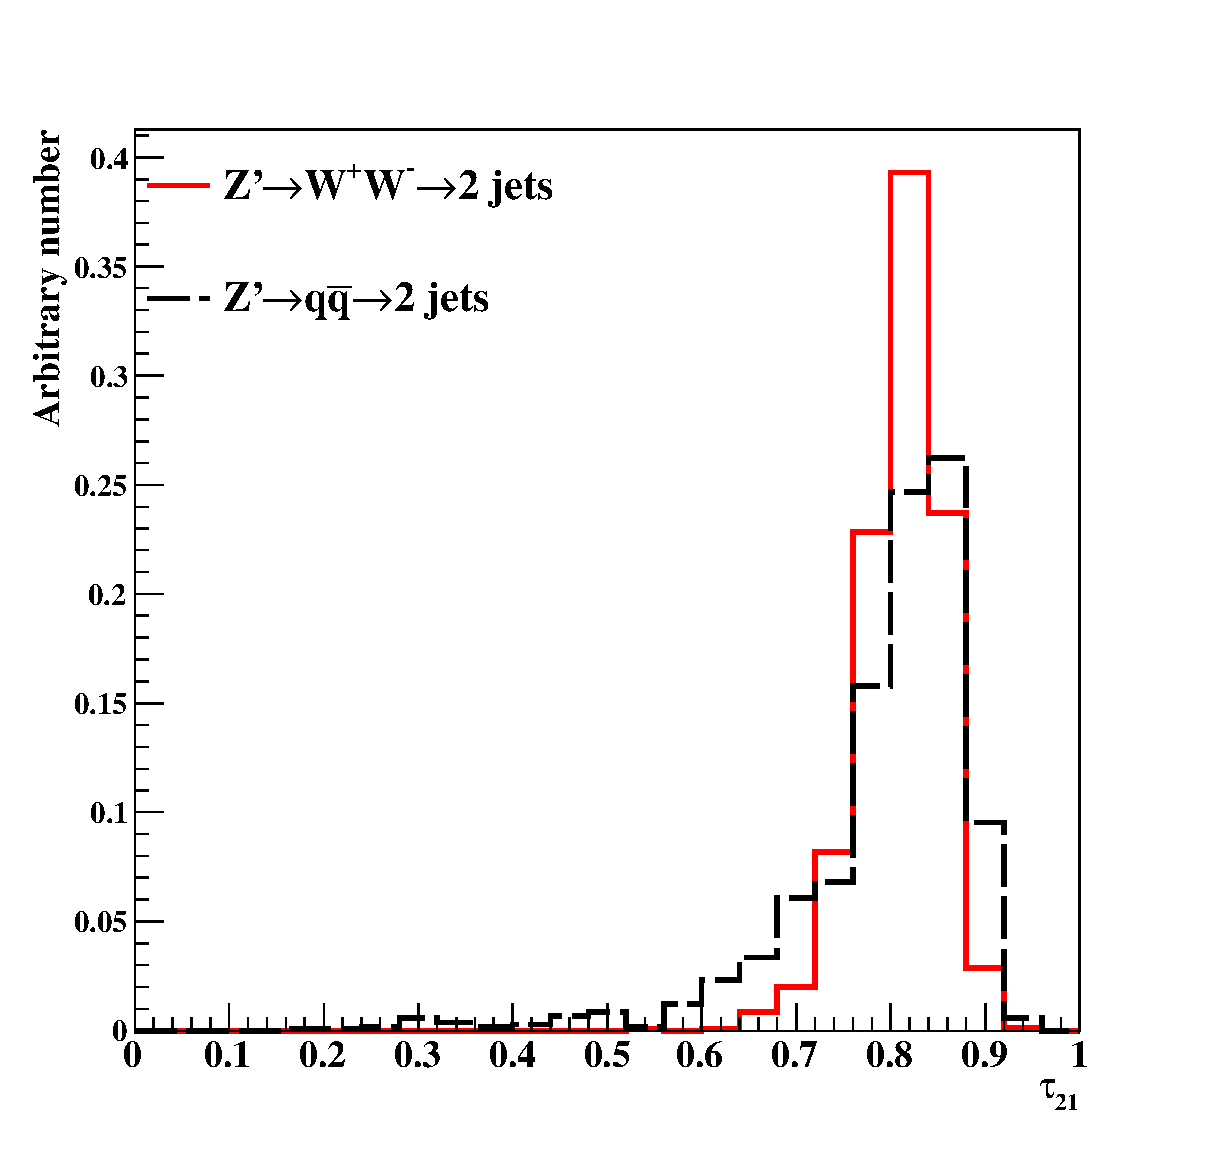
\includegraphics[width=0.3\textwidth]{h_Tau_C/Dis_Rawhit_05GeV_010_tau21_20tev_04_after_cut_Man_25_no_UOF_new_75pa_for_paper.eps}
   }
   \subfigure[5$\times$5 (cm$^2$)] {
   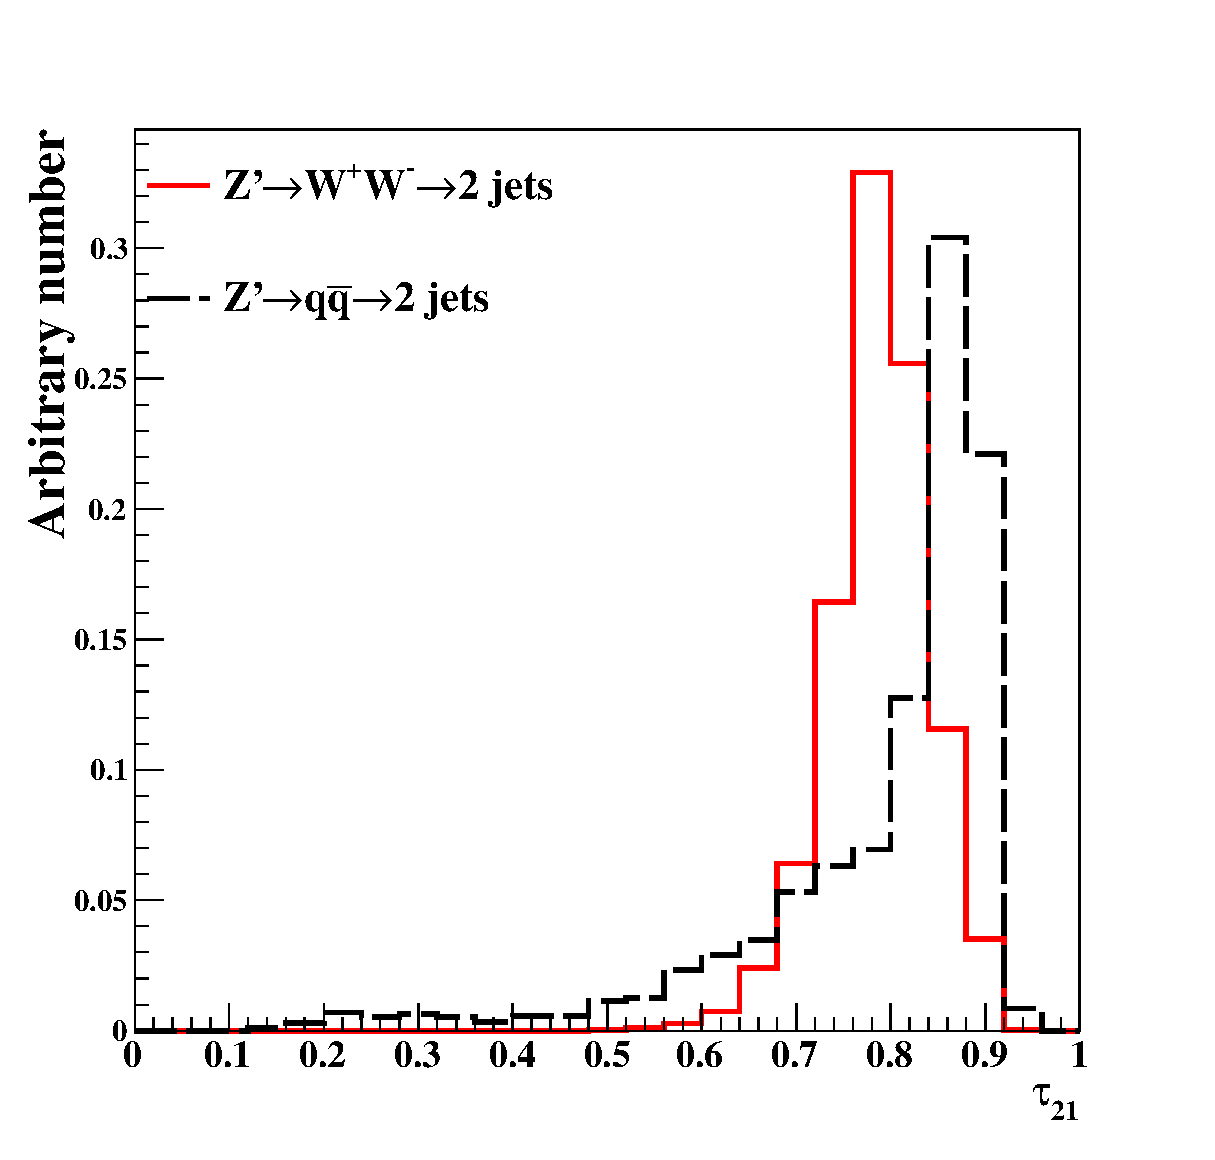
\includegraphics[width=0.3\textwidth]{h_Tau_C/Dis_Rawhit_05GeV_009_tau21_20tev_04_after_cut_Man_25_no_UOF_new_75pa_for_paper.eps}
   }
   \subfigure[1$\times$1 (cm$^2$)] {
   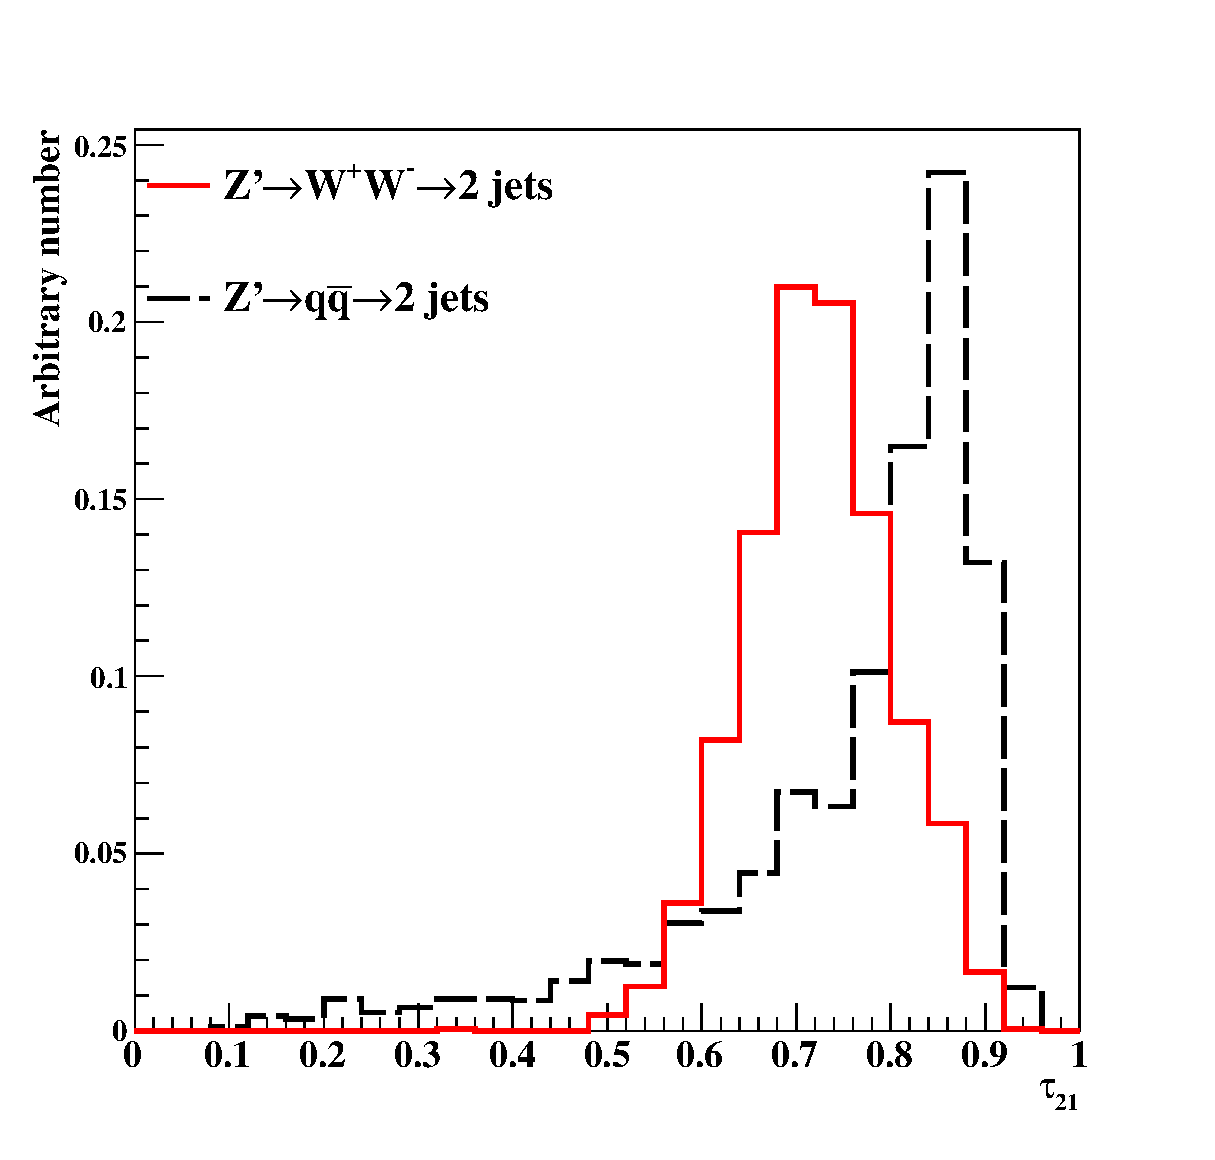
\includegraphics[width=0.3\textwidth]{h_Tau_C/Dis_Rawhit_05GeV_012_tau21_20tev_04_after_cut_Man_25_no_UOF_new_75pa_for_paper.eps}
   }
\end{center}
\caption{Distributions of $\tau_{21}$ in 20~TeV energy collision for different 
detector sizes. Cell sizes in 20$\times$20, 5$\times$5, and 1$\times$1~cm$^2$ 
are shown here. \label{fig:Rawhit_05GeV_tau21_Dis}}
\end{figure}

\begin{figure}
\begin{center}
   \subfigure[Z'(5 TeV)] {
   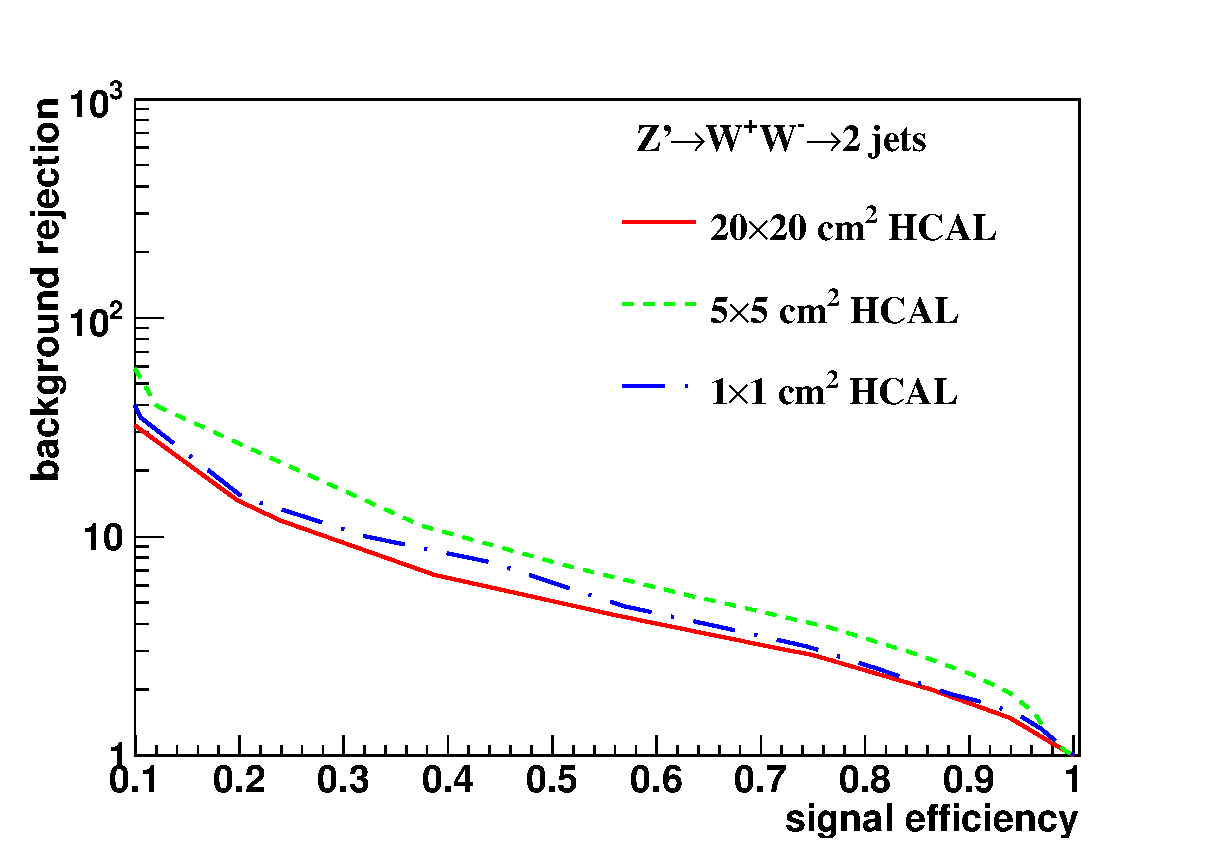
\includegraphics[width=0.43\textwidth]{ROC_Tau_C/Rawhit_05GeV_tau21_5tev_eff_1_New2_after_cut_25bins_no_UOF_new_75pa.eps}
   }
   \subfigure[Z'(10 TeV)] {
   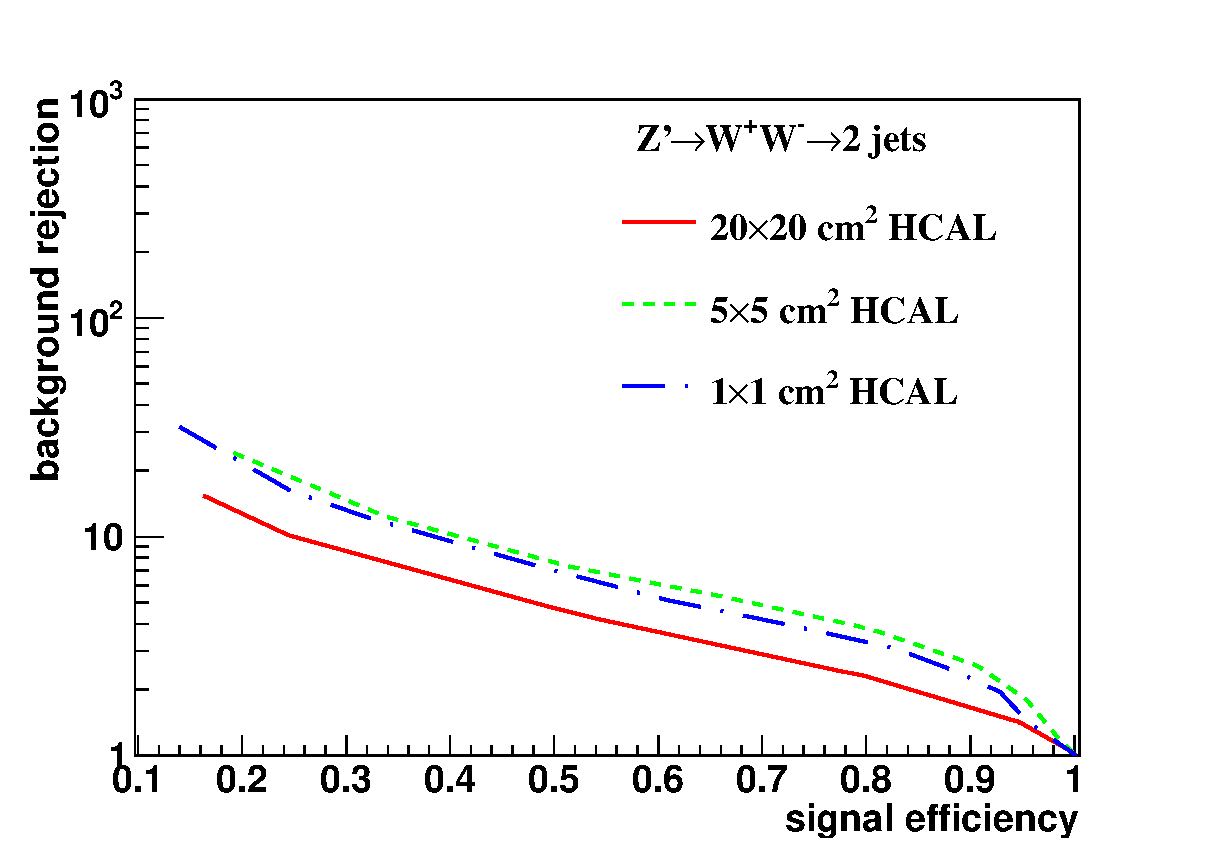
\includegraphics[width=0.43\textwidth]{ROC_Tau_C/Rawhit_05GeV_tau21_10tev_eff_1_New2_after_cut_25bins_no_UOF_new_75pa.eps}
   }
   \subfigure[Z'(20 TeV)] {
   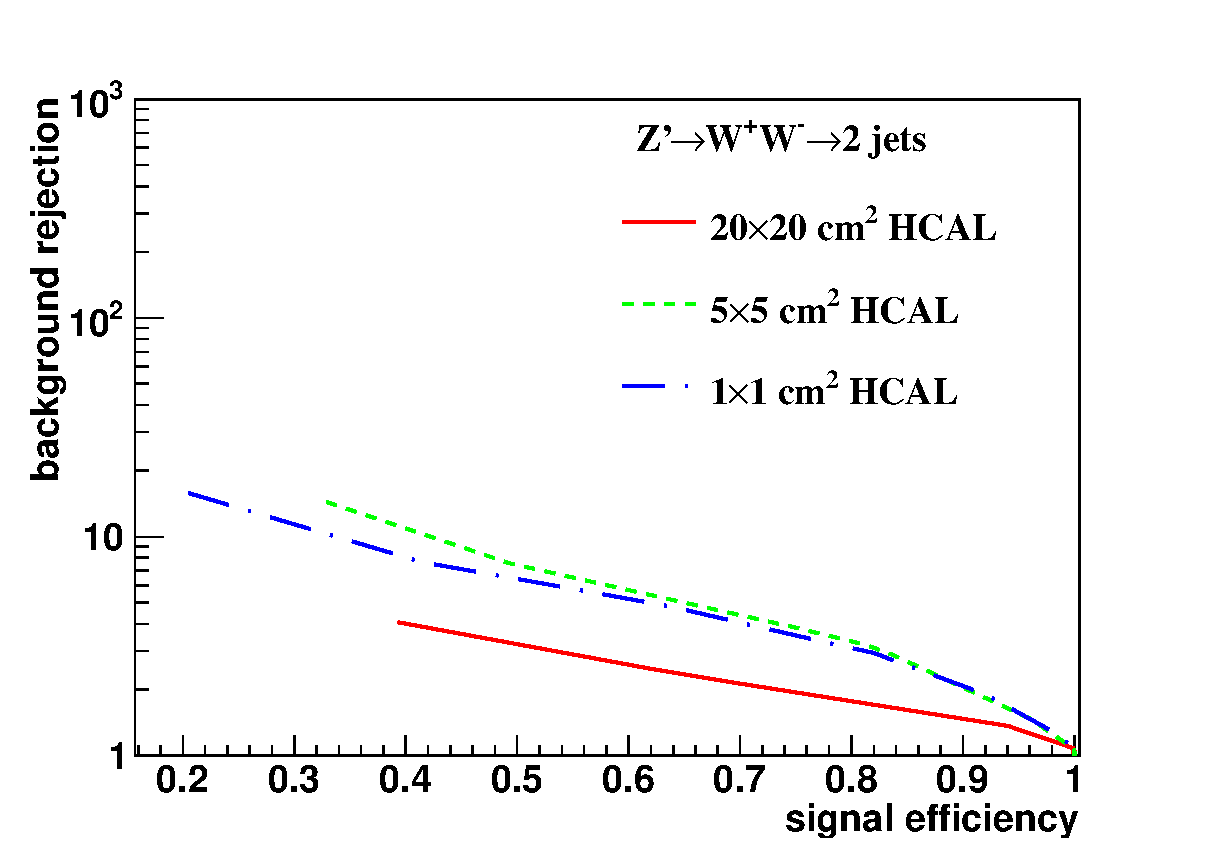
\includegraphics[width=0.43\textwidth]{ROC_Tau_C/Rawhit_05GeV_tau21_20tev_eff_1_New2_after_cut_25bins_no_UOF_new_75pa.eps}
   }
   \subfigure[Z'(40 TeV)] {
   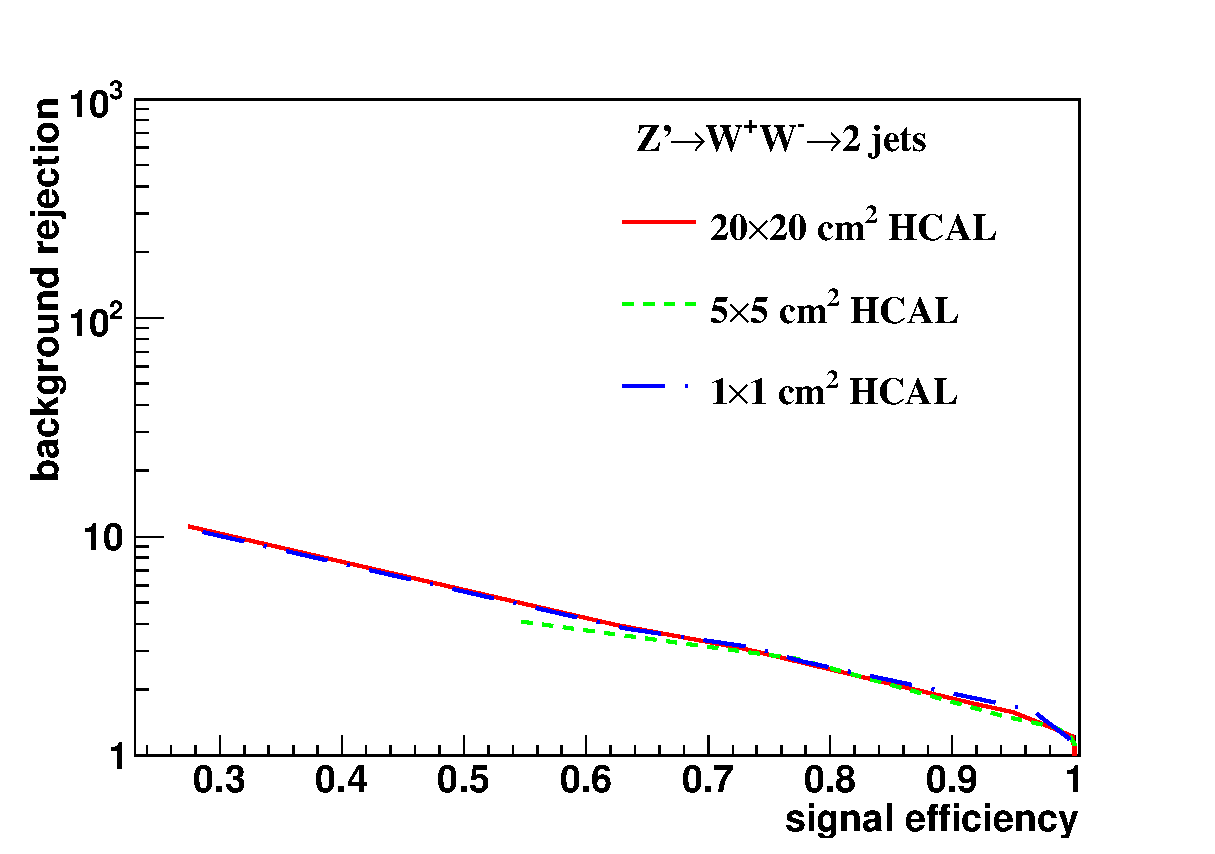
\includegraphics[width=0.43\textwidth]{ROC_Tau_C/Rawhit_05GeV_tau21_40tev_eff_1_New2_after_cut_25bins_no_UOF_new_75pa.eps}
   }
\end{center}
\caption{Signal efficiency versus background rejection rate using $\tau_{21}$.
The energies of collision at (a) 5, (b) 10, (c) 20, and (d) 40~TeV are shown 
here. 
In each figure, the three ROC curves correspond to different detector sizes.
\label{fig:Rawhit_05GeV_tau21_ROC}
}
\end{figure}



%%%%%%%%%% Tau32
%25bins
\begin{figure}
\begin{center}
   \subfigure[20$\times$20 ($cm^2$)] {
   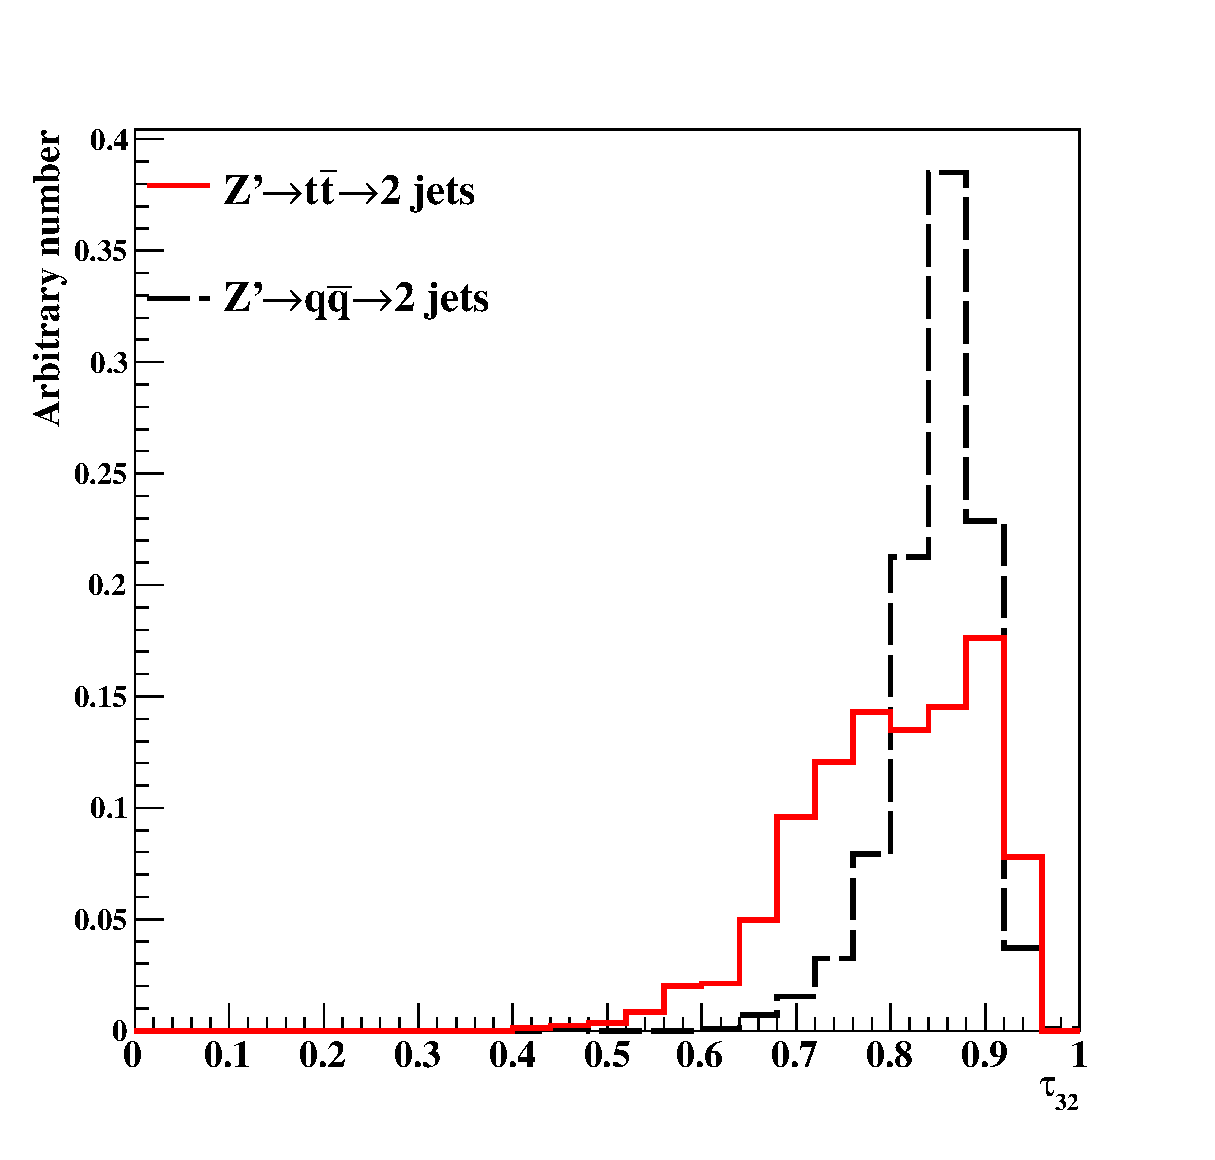
\includegraphics[width=0.3\textwidth]{h_Tau_C/Dis_Rawhit_05GeV_010_tau32_20tev_04_after_cut_Man_25_no_UOF_new_75pa_for_paper.eps}
   }
   \subfigure[5$\times$5 ($cm^2$)] {
   \includegraphics[width=0.3\textwidth]{h_Tau_C/Dis_Rawhit_05GeV_009_tau32_20tev_04_after_cut_Man_25_no_UOF_new_75pa_for_paper.eps}
   }
   \subfigure[1$\times$1 ($cm^2$)] {
   \includegraphics[width=0.3\textwidth]{h_Tau_C/Dis_Rawhit_05GeV_012_tau32_20tev_04_after_cut_Man_25_no_UOF_new_75pa_for_paper.eps}
   }
\end{center}
\caption{Distributions of $\tau_{32}$ in 20 TeV energy collision for different 
detector sizes. Cell sizes in 20$\times$20, 5$\times$5, and 1$\times$1~cm$^2$ 
are shown here.
\label{fig:Rawhit_05GeV_tau32_Dis}
}
\end{figure}

\begin{figure}
\begin{center}
   \subfigure[Z'(5 TeV)] {
   \includegraphics[width=0.43\textwidth]{ROC_Tau_C/Rawhit_05GeV_tau32_5tev_eff_1_New2_after_cut_25bins_no_UOF_new_75pa.eps}\hfill
   }
   \subfigure[Z'(10 TeV)] {
   \includegraphics[width=0.43\textwidth]{ROC_Tau_C/Rawhit_05GeV_tau32_10tev_eff_1_New2_after_cut_25bins_no_UOF_new_75pa.eps}
   }
   \subfigure[Z'(20 TeV)] {
   \includegraphics[width=0.43\textwidth]{ROC_Tau_C/Rawhit_05GeV_tau32_20tev_eff_1_New2_after_cut_25bins_no_UOF_new_75pa.eps}
   }
   \subfigure[Z'(40 TeV)] {
   \includegraphics[width=0.43\textwidth]{ROC_Tau_C/Rawhit_05GeV_tau32_40tev_eff_1_New2_after_cut_25bins_no_UOF_new_75pa.eps}
   }
\end{center}
\caption{Signal efficiency versus background rejection rate using $\tau_{32}$. 
The energies of collision at (a) 5, (b) 10, (c) 20, and (d) 40~TeV are shown 
here. In each figure, the three ROC curves correspond to different detector 
sizes.
\label{fig:Rawhit_05GeV_tau32_ROC}
}
\end{figure}


%%%%%%%%%%%%%%% c2b1
%25bins 
\begin{figure}
\centering
\begin{center}
   \subfigure[20$\times$20 ($cm^2$)] {
   \centering
   \includegraphics[width=0.3\textwidth]{h_Tau_C/Dis_Rawhit_05GeV_010_c2b1_20tev_04_after_cut_Man_25_no_UOF_new_75pa_for_paper.eps}
   }
   \subfigure[5$\times$5 ($cm^2$)] {
   \centering
   \includegraphics[width=0.3\textwidth]{h_Tau_C/Dis_Rawhit_05GeV_009_c2b1_20tev_04_after_cut_Man_25_no_UOF_new_75pa_for_paper.eps}
   }
   \subfigure[1$\times$1 ($cm^2$)] {
   \centering
   \includegraphics[width=0.3\textwidth]{h_Tau_C/Dis_Rawhit_05GeV_012_c2b1_20tev_04_after_cut_Man_25_no_UOF_new_75pa_for_paper.eps}
   }
\end{center}
\caption{Distributions of $C_2^1$ in 20~TeV energy collision for different 
detector sizes. Cell sizes in 20$\times$20, 5$\times$5, and 1$\times$1~cm$^2$ 
are shown here.}
\label{fig:Rawhit_05GeV_c2b1_Dis}
\end{figure}

\begin{figure}
\begin{center}
   \subfigure[Z'(5 TeV)] {
   \includegraphics[width=0.43\textwidth]{ROC_Tau_C/Rawhit_05GeV_c2b1_5tev_eff_1_New2_after_cut_25bins_no_UOF_new_75pa.eps}\hfill
   }
   \subfigure[Z'(10 TeV)] {
   \includegraphics[width=0.43\textwidth]{ROC_Tau_C/Rawhit_05GeV_c2b1_10tev_eff_1_New2_after_cut_25bins_no_UOF_new_75pa.eps}
   }
   \subfigure[Z'(20 TeV)] {
   \includegraphics[width=0.43\textwidth]{ROC_Tau_C/Rawhit_05GeV_c2b1_20tev_eff_1_New2_after_cut_25bins_no_UOF_new_75pa.eps}
   }
   \subfigure[Z'(40 TeV)] {
   \includegraphics[width=0.43\textwidth]{ROC_Tau_C/Rawhit_05GeV_c2b1_40tev_eff_1_New2_after_cut_25bins_no_UOF_new_75pa.eps}
   }
\end{center}
\caption{Signal efficiency versus background rejection rate using $C_{2}^{1}$. 
The energies of collision at (a) 5, (b) 10, (c) 20, and (d) 40~TeV are shown 
here. In each figure, the three ROC curves correspond to different detector 
sizes.}
\label{fig:Rawhit_05GeV_c2b1_ROC}
\end{figure}



%25bins Mann-Whitney
\begin{figure}
\begin{center}
   \subfigure[$\tau_{21}$] {
   \includegraphics[width=0.3\textwidth]{Mann_Sum/raw_05_tau21_summary_U_after_cut_25bins_no_UOF_new_75pa.eps}\hfill
   }
   \subfigure[$\tau_{32}$ ] {
   \includegraphics[width=0.3\textwidth]{Mann_Sum/raw_05_tau32_summary_U_after_cut_25bins_no_UOF_new_75pa.eps}
   }
   \subfigure[$C_2^{(1)}$] {
   \includegraphics[width=0.3\textwidth]{Mann_Sum/raw_05_c2b1_summary_U_after_cut_25bins_no_UOF_new_75pa.eps}
   }
   \end{center}
\caption{The Mann-Whitney U values for $\tau_{21}$, $\tau_{32}$, and $C_2^{(1)}$ 
reconstructed with different collision energies and detector cell sizes. }
\label{fig:Rawhit_05GeV_total_Mann}
\end{figure}














\section*{Acknowledgements}
This research was performed using resources provided by the Open Science Grid,
which is supported by the National Science Foundation and the U.S. Department of Energy's Office of Science. 
We gratefully acknowledge the computing resources provided on Blues, 
a high-performance computing cluster operated by the Laboratory Computing Resource Center at Argonne National Laboratory.
Argonne National Laboratory's work was supported by the U.S. Department of Energy, Office of Science under contract DE-AC02-06CH11357.
The Fermi National Accelerator Laboratory (Fermilab) is operated by Fermi Research Alliance, LLC under Contract No. DE-AC02-07CH11359 with the United States Department of Energy.

\newpage
%%%%%%%%%%%%%%%%%%%%%% references %%%%%%%%%%%%%%%%%%%%%%%%%%%%%%
\section*{References}

\bibliographystyle{elsarticle-num}
\def\bibname{\Large\bf References}
\def\refname{\Large\bf References}
\pagestyle{plain}
\bibliography{biblio}



\end{document}
